\documentclass{article}

% Packages
\usepackage[margin=1.5cm, includefoot, footskip=30pt]{geometry}
\usepackage{hyperref}
\usepackage{multicol}
\usepackage{booktabs}
\usepackage{xstring}
\usepackage{subcaption}
\usepackage{graphicx}
\usepackage{amsmath}
\usepackage{standalone}
\usepackage{fancyvrb}

\usepackage{tikz}
\usetikzlibrary{calc, shapes, patterns}

\usepackage[backend=biber, firstinits=false, backref=false, url=true,
            isbn=true, style=numeric]{biblatex}
\addbibresource{./tex/bibliography.bib}

% Title
\title{An empirical study of fixation for strategies in the
       Iterated Prisoner's Dilemma}
\author{Marc Harper \and Vincent Knight \and Nikoleta E. Glynatsi} % TODO Authors?
\date{}


\begin{document}

\maketitle

\begin{abstract}
    The Iterated Prisoner's Dilemma is a well established framework for
    the study of emergent behaviour. In this paper an extensive numerical
    study of the evolutionary dynamics of this framework are presented.

    Fixation probabilities for Moran processes are obtained for 164
    different strategies.

    To the authors knowledge this is the largest
    such study. It allows for insights about the behaviour and
    performance of strategies with regard to their survival in an
    evolutionary setting.

    Evidence is presented that shows that classical analysis of evolutionary
    dynamics with 2 individuals is misleading. Furthermore, it is shown that
    players with long memories and sophisticated behaviours outperform many
    strategies that perform well in a 2 individual setting (such as zero
    determinant strategies).

\end{abstract}

\section{Introduction}\label{sec:introduction}

The Prisoner's Dilemma (PD)~\cite{Flood1958} is a fundamental two person game 
in Game theory. Each player can choose between cooperation (C) or defection 
(D). The decisions are made simultaneously and independently. The payoffs of
the game are defined by the matrix $\begin{pmatrix} R & S \\ T & P
\end{pmatrix}$, where $T > R > P> S$ and $2R > T + S$. The PD is a one 
round game, but is commonly studied in a manner where the prior outcomes 
matter, the game then extends to its `iterated'\ form, the Iterated Prisoner's 
Dilemma (IPD). 

Since the formulation of the Moran Process in \cite{Moran1957}, this model of
evolutionary population dynamics has been used to gain insights about the
evolutionary stability of strategies in a number of settings. Similarly since
the first Iterated Prisoner's Dilemma (IPD) tournament described in
\cite{Axelrod1980a} the Prisoner's dilemma has been used to understand the
evolution of cooperative behaviour in complex systems.

The analytical models of a Moran process are based on the relative fitness
between two strategies and take this to be a fixed value \(r\) \cite{Nowak}.
This is a valid model for simple strategies of the Prisoner's Dilemma such as to
\textit{always cooperate} or \textit{always defect}. This manuscript provides a
detailed numerical analysis of \textbf{164} complex and adaptive strategies for
the IPD\@. In this case the relative fitness of a strategy is dependent on the
population distribution.

Further deviations from the analytical model occur when interactions between
players are subject to uncertainty. This is referred to as noise and has been
considered in the IPD setting in \cite{Bendor1993, Nowak1993, Wu1995}.

This work provides answers to the following questions:

\begin{enumerate}
    \item What strategies are good invaders?
    \item What strategies are good at resisting invasion?
    \item How does the population size affect these findings?
\end{enumerate}

Figure~\ref{fig:moran_process} shows a diagrammatic representation of the Moran
process. This process is a stochastic birth death process on a finite population
in which the population size stays constant over time. Individuals are
\textbf{selected} according to a given fitness landscape. Once selected, a given
individual is reproduced and similarly another individual is chosen to be
removed from the population. In some settings mutation is also considered but
without mutation (the case considered in this work) this process will arrive at
an absorbing state where the population is entirely made up of a single
individual. The probability with which a given strategy is the survivor is
called the fixation probability. A more detailed analytic description of this
is given in Section~\ref{sec:validation}.

\begin{figure}[!hbtp]
    \centering
    \documentclass{standalone}
\usepackage{tikz}
\usetikzlibrary{calc, shapes, patterns}

\begin{document}
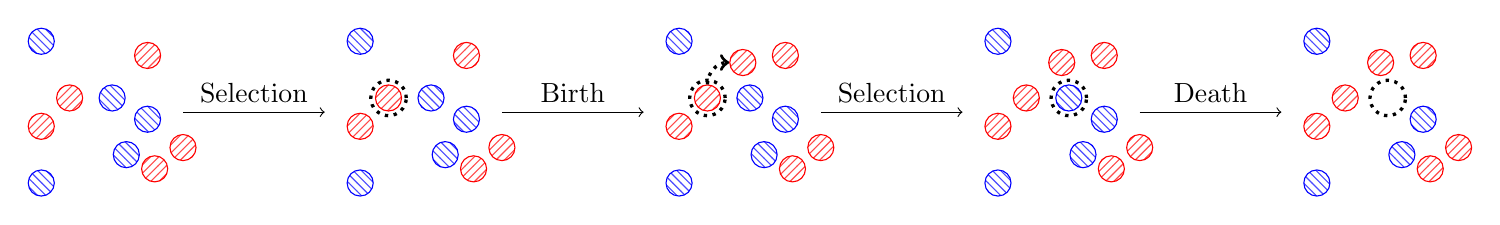
\begin{tikzpicture}[scale=.9]
	\node (A1) at (-1, -1) [circle, pattern=north west lines, pattern
        color=blue!70, draw=blue] {};
	\node (A2) at (-1, 1) [circle, pattern=north west lines, pattern
        color=blue!70, draw=blue] {};
	\node (A3) at (0, .2) [circle, pattern=north west lines, pattern
        color=blue!70, draw=blue] {};
	\node (A4) at (.2, -.6) [circle, pattern=north west lines, pattern
        color=blue!70, draw=blue] {};
	\node (A5) at (.5, -0.1) [circle, pattern=north west lines, pattern
        color=blue!70, draw=blue] {};
	\node (B1) at (-1, -.2) [circle, pattern=north east lines, pattern
        color=red!70, draw=red] {};
	\node (B2) at (1, -.5) [circle, pattern=north east lines, pattern
        color=red!70, draw=red] {};
	\node (B3) at (.5, .8) [circle, pattern=north east lines, pattern
        color=red!70, draw=red] {};
	\node (B4) at (-.6, .2) [circle, pattern=north east lines, pattern
        color=red!70, draw=red] {};
	\node (B5) at (.6, -.8) [circle, pattern=north east lines, pattern
        color=red!70, draw=red] {};

	\draw [->] (1, 0) -- (3, 0) node [above, pos=0.5] {Selection};

	\node (A1) at ($(A1) + (4.5, 0)$) [circle, pattern=north west lines,
        pattern color=blue!70, draw=blue] {};
	\node (A2) at ($(A2) + (4.5, 0)$) [circle, pattern=north west lines,
        pattern color=blue!70, draw=blue] {};
	\node (A3) at ($(A3) + (4.5, 0)$) [circle, pattern=north west lines,
        pattern color=blue!70, draw=blue] {};
	\node (A4) at ($(A4) + (4.5, 0)$) [circle, pattern=north west lines,
        pattern color=blue!70, draw=blue] {};
    \node (A5) at ($(A5) + (4.5, 0)$) [circle, pattern=north west lines,
        pattern color=blue!70, draw=blue] {};
	\node (B1) at ($(B1) + (4.5, 0)$) [circle, pattern=north east lines,
        pattern color=red!70, draw=red] {};
	\node (B2) at ($(B2) + (4.5, 0)$) [circle, pattern=north east lines,
        pattern color=red!70, draw=red] {};
	\node (B3) at ($(B3) + (4.5, 0)$) [circle, pattern=north east lines,
        pattern color=red!70, draw=red] {};
	\node (B4) at ($(B4) + (4.5, 0)$) [circle, pattern=north east lines,
        pattern color=red!70, draw=red] {};
	\node (B5) at ($(B5) + (4.5, 0)$) [circle, pattern=north east lines,
        pattern color=red!70, draw=red] {};

	\draw [dotted, very thick] (B4) circle (.25cm);

	\draw [->] (5.5, 0) -- (7.5, 0) node [above, pos=0.5] {Birth};

	\node (A1) at ($(A1) + (4.5, 0)$) [circle, pattern=north west lines,
        pattern color=blue!70, draw=blue] {};
	\node (A2) at ($(A2) + (4.5, 0)$) [circle, pattern=north west lines,
        pattern color=blue!70, draw=blue] {};
	\node (A3) at ($(A3) + (4.5, 0)$) [circle, pattern=north west lines,
        pattern color=blue!70, draw=blue] {};
	\node (A4) at ($(A4) + (4.5, 0)$) [circle, pattern=north west lines,
        pattern color=blue!70, draw=blue] {};
    \node (A5) at ($(A5) + (4.5, 0)$) [circle, pattern=north west lines,
        pattern color=blue!70, draw=blue] {};
	\node (B1) at ($(B1) + (4.5, 0)$) [circle, pattern=north east lines,
        pattern color=red!70, draw=red] {};
	\node (B2) at ($(B2) + (4.5, 0)$) [circle, pattern=north east lines,
        pattern color=red!70, draw=red] {};
	\node (B3) at ($(B3) + (4.5, 0)$) [circle, pattern=north east lines,
        pattern color=red!70, draw=red] {};
	\node (B4) at ($(B4) + (4.5, 0)$) [circle, pattern=north east lines,
        pattern color=red!70, draw=red] {};
	\node (B5) at ($(B5) + (4.5, 0)$) [circle, pattern=north east lines,
        pattern color=red!70, draw=red] {};

	\draw [dotted, very thick] (B4) circle (.25cm);
	\node (B6) at ($(B4) + (0.5, 0.5)$) [circle, pattern=north east lines,
        pattern color=red!70, draw=red] {};
	\draw [->, dotted, very thick] (B4) [out=90, in=180] to (B6);

	\draw [->] (10, 0) -- (12, 0) node [above, pos=0.5] {Selection};

	\node (A1) at ($(A1) + (4.5, 0)$) [circle, pattern=north west lines,
        pattern color=blue!70, draw=blue] {};
	\node (A2) at ($(A2) + (4.5, 0)$) [circle, pattern=north west lines,
        pattern color=blue!70, draw=blue] {};
	\node (A3) at ($(A3) + (4.5, 0)$) [circle, pattern=north west lines,
        pattern color=blue!70, draw=blue] {};
	\node (A4) at ($(A4) + (4.5, 0)$) [circle, pattern=north west lines,
        pattern color=blue!70, draw=blue] {};
    \node (A5) at ($(A5) + (4.5, 0)$) [circle, pattern=north west lines,
        pattern color=blue!70, draw=blue] {};
	\node (B1) at ($(B1) + (4.5, 0)$) [circle, pattern=north east lines,
        pattern color=red!70, draw=red] {};
	\node (B2) at ($(B2) + (4.5, 0)$) [circle, pattern=north east lines,
        pattern color=red!70, draw=red] {};
	\node (B3) at ($(B3) + (4.5, 0)$) [circle, pattern=north east lines,
        pattern color=red!70, draw=red] {};
	\node (B4) at ($(B4) + (4.5, 0)$) [circle, pattern=north east lines,
        pattern color=red!70, draw=red] {};
	\node (B5) at ($(B5) + (4.5, 0)$) [circle, pattern=north east lines,
        pattern color=red!70, draw=red] {};
	\node (B6) at ($(B6) + (4.5, 0)$) [circle, pattern=north east lines,
        pattern color=red!70, draw=red] {};

	\draw [dotted, very thick] (A3) circle (.25cm);

	\draw [->] (14.5, 0) -- (16.5, 0) node [above, pos=0.5] {Death};

	\node (A1) at ($(A1) + (4.5, 0)$) [circle, pattern=north west lines,
        pattern color=blue!70, draw=blue] {};
	\node (A2) at ($(A2) + (4.5, 0)$) [circle, pattern=north west lines,
        pattern color=blue!70, draw=blue] {};
	\node (A3) at ($(A3) + (4.5, 0)$) {};
	\node (A4) at ($(A4) + (4.5, 0)$) [circle, pattern=north west lines,
        pattern color=blue!70, draw=blue] {};
    \node (A5) at ($(A5) + (4.5, 0)$) [circle, pattern=north west lines,
        pattern color=blue!70, draw=blue] {};
	\node (B1) at ($(B1) + (4.5, 0)$) [circle, pattern=north east lines,
        pattern color=red!70, draw=red] {};
	\node (B2) at ($(B2) + (4.5, 0)$) [circle, pattern=north east lines,
        pattern color=red!70, draw=red] {};
	\node (B3) at ($(B3) + (4.5, 0)$) [circle, pattern=north east lines,
        pattern color=red!70, draw=red] {};
	\node (B4) at ($(B4) + (4.5, 0)$) [circle, pattern=north east lines,
        pattern color=red!70, draw=red] {};
	\node (B5) at ($(B5) + (4.5, 0)$) [circle, pattern=north east lines,
        pattern color=red!70, draw=red] {};
	\node (B6) at ($(B6) + (4.5, 0)$) [circle, pattern=north east lines,
        pattern color=red!70, draw=red] {};

	\draw [dotted, very thick] (A3) circle (.25cm);
\end{tikzpicture}
\end{document}

    \caption{A diagrammatic representation of a Moran process}
    \label{fig:moran_process}
\end{figure}

The Moran process was initially introduced in \cite{Moran1957} in a genetic
setting. It has since been used in a variety of settings including the
understanding of the spread of cooperative behaviour. For instance, cancer 
cells \cite{West2016}. Emergence of cooperative behaviour, also includes 
studies in spatial topologies \cite{Nowak2017}. However, as stated before, 
these mainly consider non sophisticated strategies. Some work has looked at
evolutionary stability of strategies within the Prisoner's Dilemma \cite{Li2014}
but this is not done in the more widely used setting of the Moran process but in
terms of infinite population stability. In \cite{Baek2016} Moran processes are
looked at in a theoretic framework for a small subset of strategies. 
The subset included memory one strategies, strategies that recall the events 
of the previous round only. In \cite{Press2012}, a set of memory one 
strategies, the zero determinant strategies, were introduced. The ZD\@,
strategies are highly praised and in \cite{Stewart26062012} argued that 
generous ZD strategies are robust against invading strategies. However,
in \cite{Lee2015} machine learning techniques are used to train a strategy 
capable of resisting invasion and also able to invade any memory one strategy. 
Recent work \cite{Hilbe2017} has investigated the effect of memory length on 
strategy performance and the emergence of cooperation but this is not done in 
Moran process context and only considers specific cases of memory 2 strategies.
% TODO Add discussion about ZD strategies and discuss how this corresponds to
% case of N = 2. Include pointing at \cite{Adami2013} which discusses how ZD
% strategies are not fantastic in population dynamics.
% Add \cite{Li2014}

The contribution of this work is a detailed and extensive analysis of absorption
probabilities for 164 strategies. These strategies and the numerical simulations
are from~\cite{axelrodproject} which is an open source research library written
for the study of the IPD\@. The strategies and simulation frameworks are
automatically tested in accordance to best research software practice. The large
number of strategies are available thanks to the open source nature of the
project with over 40 contributions made by different programmers. Thus by
considering Moran processes with population size greater than 2 we are taking in
to account the effect of complex population dynamics. By considering
sophisticated strategies we are taking in to effect the reputation of a strategy
during each interaction.

Section~\ref{sec:methodology} will explain the methodological approach used,
Section~\ref{sec:validation} will validate the methodology by comparing
simulated results to analytical results. The main results of this manuscript are
presented in Section~\ref{sec:empirical_results} which will present a detailed
analysis of all the data generated. Finally, Section~\ref{sec:conclusion} will
conclude and offer future avenues for the work presented here.

\section{Methodology}\label{sec:methodology}

To carry out this large numerical experiment 164 strategies are used from
\cite{axelrodproject}. These include 161 default strategies in the library at
the time (excluding strategies classified as having a long run time and those
that make use of the length of the game) as well as
the following 3 finite state machine machine strategies \cite{Ashlock2006}:

% TODO Include details about the 3 extra FSM strategies.
% Possibly draw pictorial representations?

Appendix~\ref{app:list_of_players} shows all the players in question. More
information about each player can be obtained in the documentation for
\cite{axelrodproject}. There are 43stochastic and
124deterministic strategies. Their memory
depth is shown in Table~\ref{tbl:memory_depth_count}.

\begin{table}[!hbtp]
    \centering
        \begin{tabular}{lrrrrrrrrrrrrrrrr}
\toprule
Memory Depth &   0   &   1   &   2   &   3   &   4   &   5   &   6   &   9   &   10  &   11  &   12  &   16  &   20  &   40  &   200 &  \(\infty\)   \\
\midrule
Count &     3 &    34 &    12 &     8 &     2 &     6 &     1 &     1 &     5 &     1 &     1 &     2 &     2 &     2 &     1 &    86 \\
\bottomrule
\end{tabular}

        \caption{Memory depth}
        \label{tbl:memory_depth_count}
\end{table}

All strategies are paired and these pairs are used in 1000 repetitions of a
Moran process assuming a starting population distribution of \(1, N-1 \),
\((N/2, N/2)\) and \(N-1 , 1\). This is repeated for \(N\) between 2 and 14. The
% TODO Change 14 to 12 if we do not use the 14 case.
fixation probability is then estimated for each value of \(N\).

Note that due to the high computational cost of these experiments, for any given
interaction between two players within the Moran process the outcome is sampled
from a pre computed cache of 1000 match outcomes. This is carried out using
software written for the purpose of this work. This has been
implemented in~\cite{axelrodproject} ensuring that it can be used to either
reproduce the work or carry out further work.
% TODO Perhaps write some pseudo code for this?

Figure~\ref{fig:number_of_stochastic_match_outcomes} shows the distribution of
the number of outcomes between all strategy pairs.
Tables~\ref{tbl:number_of_stochastic_match_outcomes} shows that 95\% of the
stochastic matches have less than 788 unique outcomes whilst the maximum number
is 971. This ensures that using a set of cached results from 1000 precomputed
matches is sufficient for the analysis taking place here.

\begin{figure}[!hbtp]
    \centering
    \begin{subfigure}[t]{.5\textwidth}
        \centering
        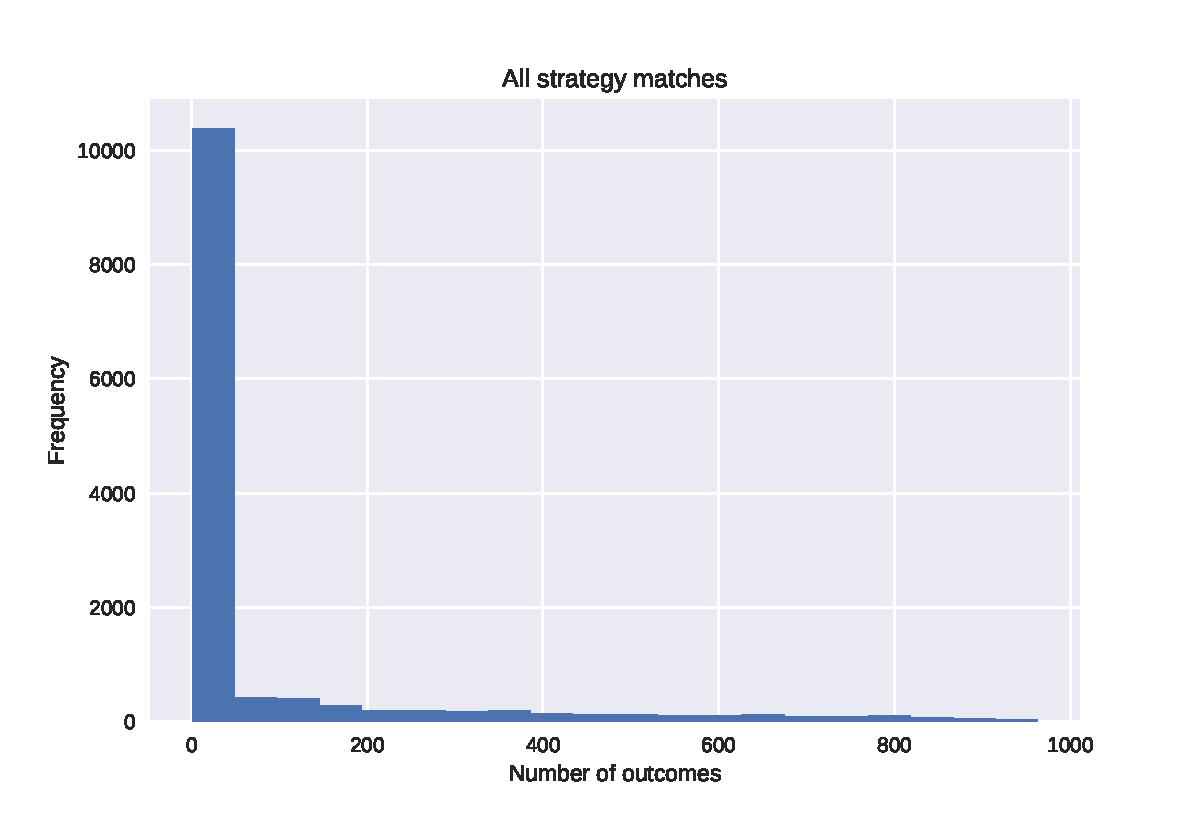
\includegraphics[width=.9\textwidth]{./img/number_of_match_outcomes.pdf}
        \caption{All matches}
    \end{subfigure}%
    ~
    \begin{subfigure}[t]{.5\textwidth}
        \centering
        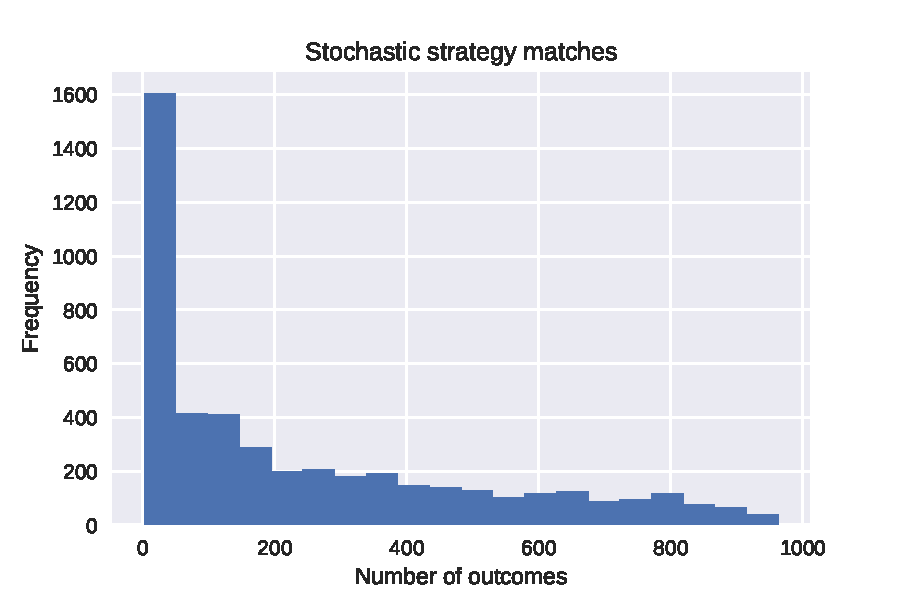
\includegraphics[width=.9\textwidth]{./img/number_of_stochastic_match_outcomes.pdf}
        \caption{Stochastic matches}
    \end{subfigure}%
    \caption{The distribution of the number of unique outcomes used as the
    cached results}
    \label{fig:number_of_stochastic_match_outcomes}
\end{figure}


\begin{table}[!hbtp]
    \centering
    \begin{subfigure}[t]{.5\textwidth}
        \centering
        \begin{tabular}{lr}
\toprule
{} &  Outcome count \\
\midrule
count &       13530.00 \\
mean  &          85.98 \\
std   &         192.58 \\
min   &           1.00 \\
25\%   &           1.00 \\
50\%   &           1.00 \\
75\%   &          36.00 \\
95\%   &         595.00 \\
max   &         971.00 \\
\bottomrule
\end{tabular}

        \caption{All matches}
    \end{subfigure}%
    ~
    \begin{subfigure}[t]{.5\textwidth}
        \centering
        \begin{tabular}{lr}
\toprule
{} &  Outcome count \\
\midrule
count &        4753.00 \\
mean  &         242.90 \\
std   &         260.04 \\
min   &           2.00 \\
25\%   &          28.00 \\
50\%   &         139.00 \\
75\%   &         394.00 \\
95\%   &         788.00 \\
max   &         971.00 \\
\bottomrule
\end{tabular}

        \caption{Stochastic matches}
    \end{subfigure}%
    \caption{Summary statistics for the number of different match outcomes used
    as the cached results}
    \label{tbl:number_of_stochastic_match_outcomes}
\end{table}

Section~\ref{sec:validation} will validate the methodology used here against
known theoretic results.

\section{Validation}\label{sec:validation}

As described in \cite{Nowak} consider the payoff matrix:

\begin{equation}\label{equ:payoff_matrix}
    M = \begin{pmatrix}
        a, b\\
        c, d
        \end{pmatrix}
\end{equation}

The expected payoffs of \(i\) players of the first type in a population with \(N
- i\) players of the second type are given by:

\begin{equation}\label{equ:expected_payoff_one}
    F_i = \frac{a(i - 1) + b(N - i)}{N - 1}
\end{equation}

\begin{equation}\label{equ:expected_payoff_two}
    G_i = \frac{ci + d(N - i - 1)}{N - 1}
\end{equation}

With an intensity of selection \(\omega\) the fitness of both strategies is
given by:

\begin{equation}\label{equ:expected_payoff_one}
    f_i = 1 - \omega + \omega F_i
\end{equation}

\begin{equation}\label{equ:expected_payoff_two}
    g_i = 1 - \omega + \omega G_i
\end{equation}

The transitions within the birth death process that underpins the Moran process
are then given by:

\begin{align}
	p_{i, i+1}&= \frac{if_i}{if_i+(N-i)g_i}\frac{N-i}{N}\label{equ:p_up}\\
	p_{i, i-1}&= \frac{(N-i)g_i}{if_i+(N-i)g_i}\frac{i}{N}\label{equ:p_down}\\
	p_{ii} &= 1 - p_{i, i+1} - p_{i, i-1}\label{equ:p_stay}
\end{align}

Using this it is a known result that the fixation probability of the first
strategy in a population of \(i\) individuals of the first type (and \(N-i\)
individuals of the second. We have:

\begin{equation}\label{equ:fixation_probability}
x_i = \frac{1 + \sum_{j=1}^{i-1}\prod_{k=1}^{j}\gamma_j}{1 + \sum_{j=1}^{N-1}
      \prod_{k=1}^{j}\gamma_j}
\end{equation}

where:

\[
\gamma_j = \frac{p_{j, j-1}}{p_{j, j+1}}
\]

Using this comparisons of \(x_1, x_{N/2}, x_{N-1}\) are shown in
Figure~\ref{fig:comparison_deterministic}. The points represent the simulated
values and the line shows the theoretic value. Note that these are all
deterministic strategies and show a perfect match up between the expected value
of (\ref{equ:fixation_probability}) and the actual Moran process for all
strategies pairs.

\begin{figure}[!hbtp]
    \centering
    \begin{subfigure}[t]{.3\textwidth}
        \centering
        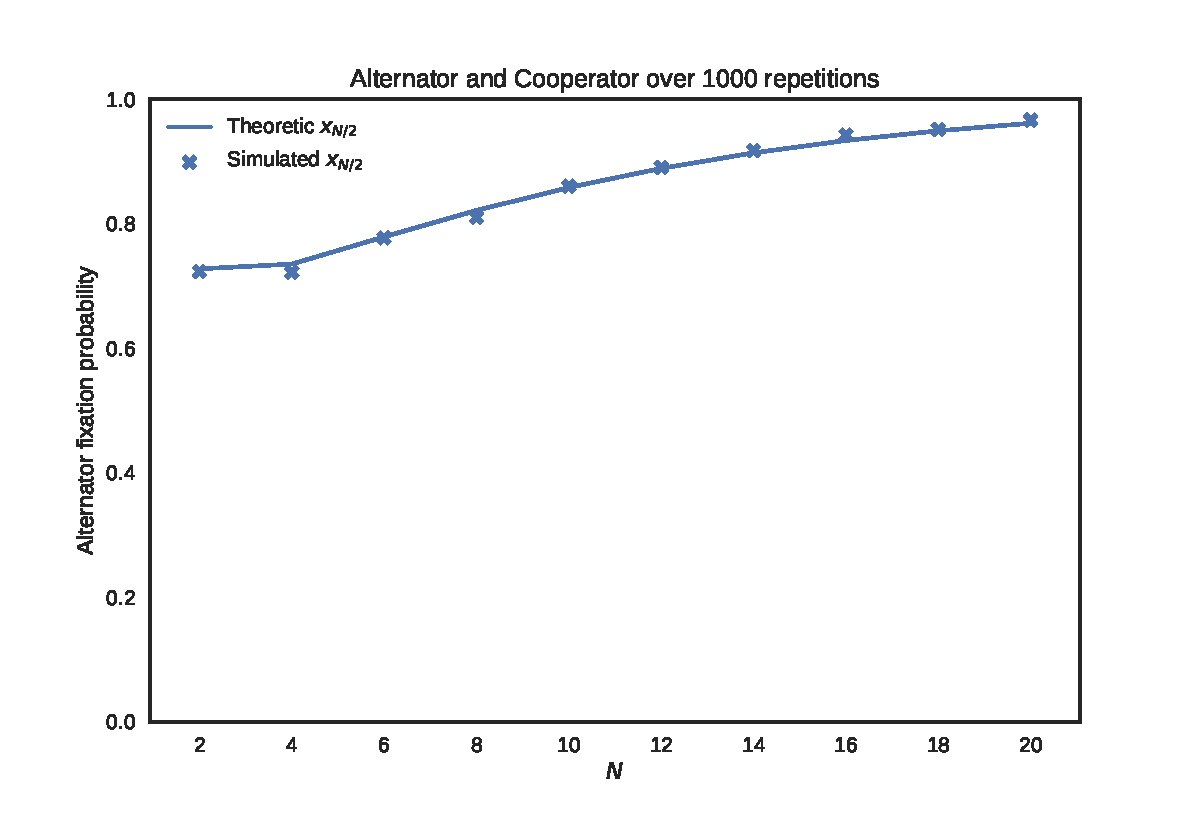
\includegraphics[width=.8\textwidth]{./img/Alternator_v_Cooperator.pdf}
        \caption{Alternator and Cooperator}
    \end{subfigure}%
    ~
    \begin{subfigure}[t]{.3\textwidth}
        \centering
        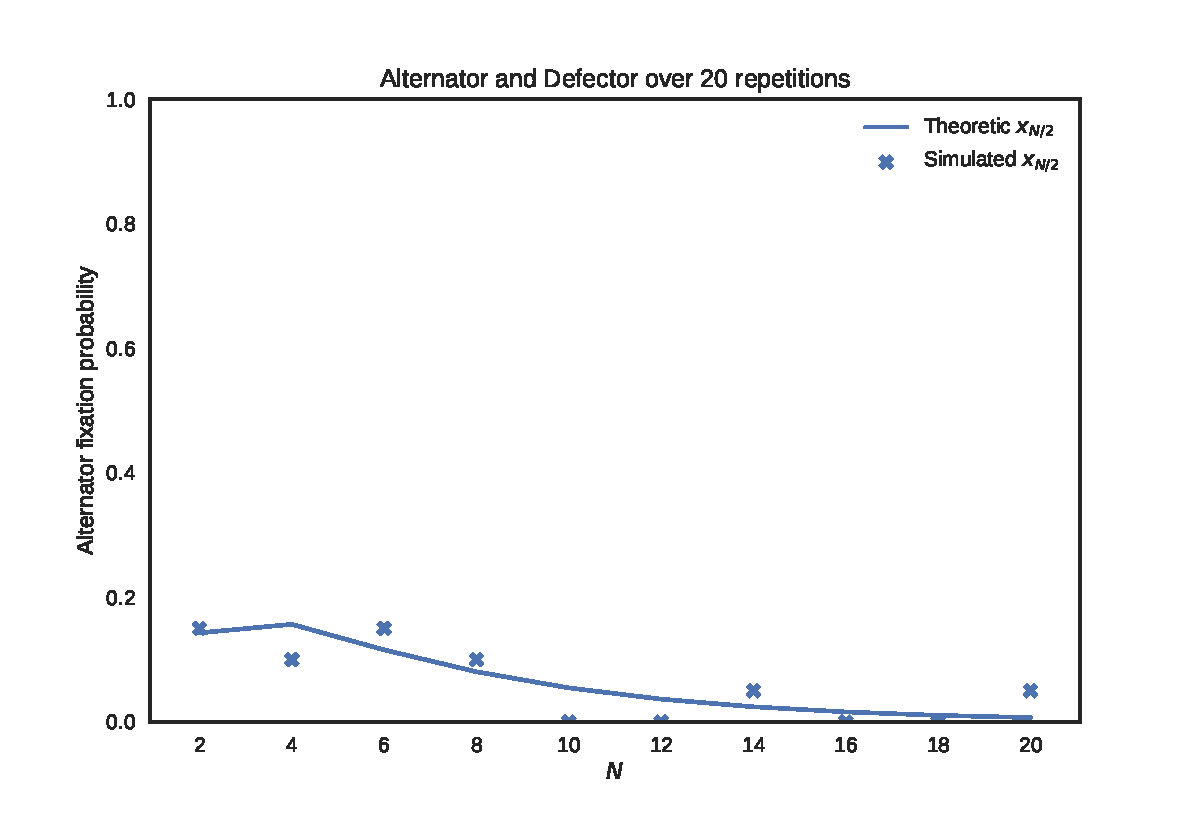
\includegraphics[width=.8\textwidth]{./img/Alternator_v_Defector.pdf}
        \caption{Alternator and Defector}
    \end{subfigure}%
    ~
    \begin{subfigure}[t]{.3\textwidth}
        \centering
        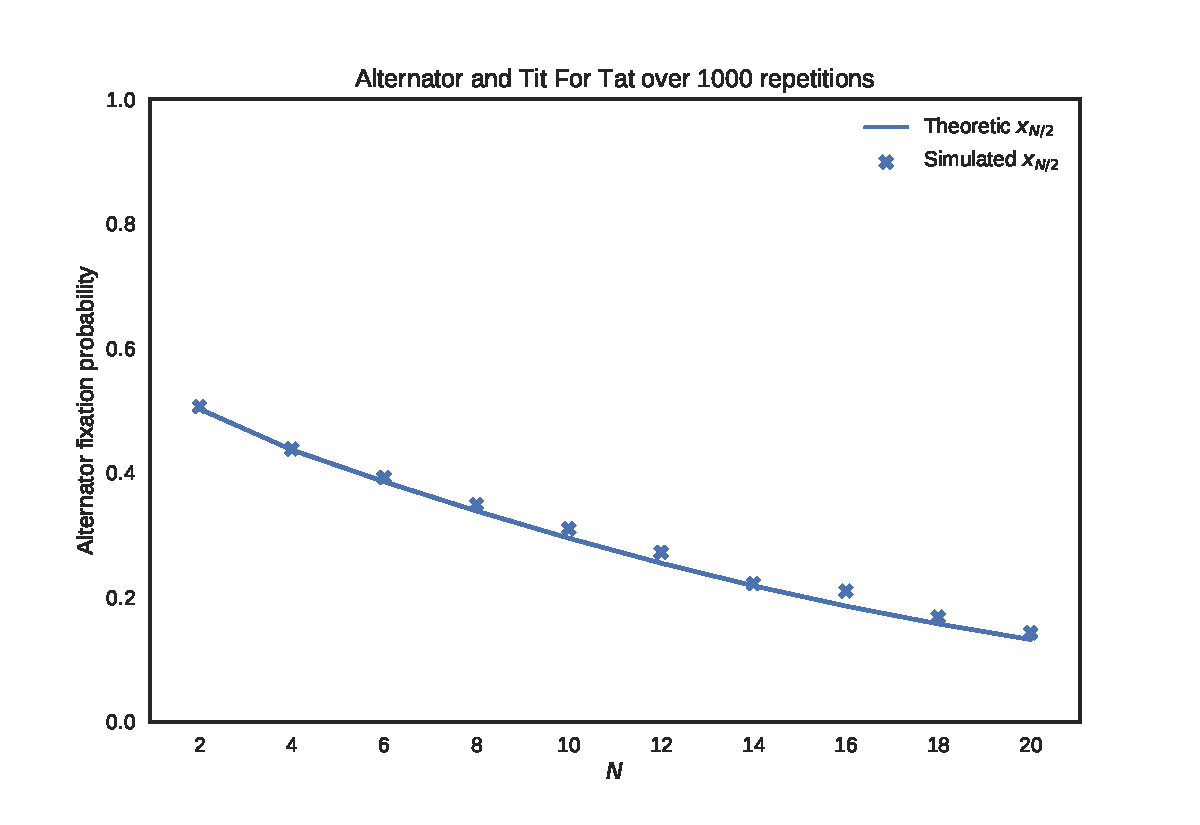
\includegraphics[width=.8\textwidth]{./img/Alternator_v_Tit_For_Tat.pdf}
        \caption{Alternator and Tit For Tat}
    \end{subfigure}%

    \begin{subfigure}[t]{.3\textwidth}
        \centering
        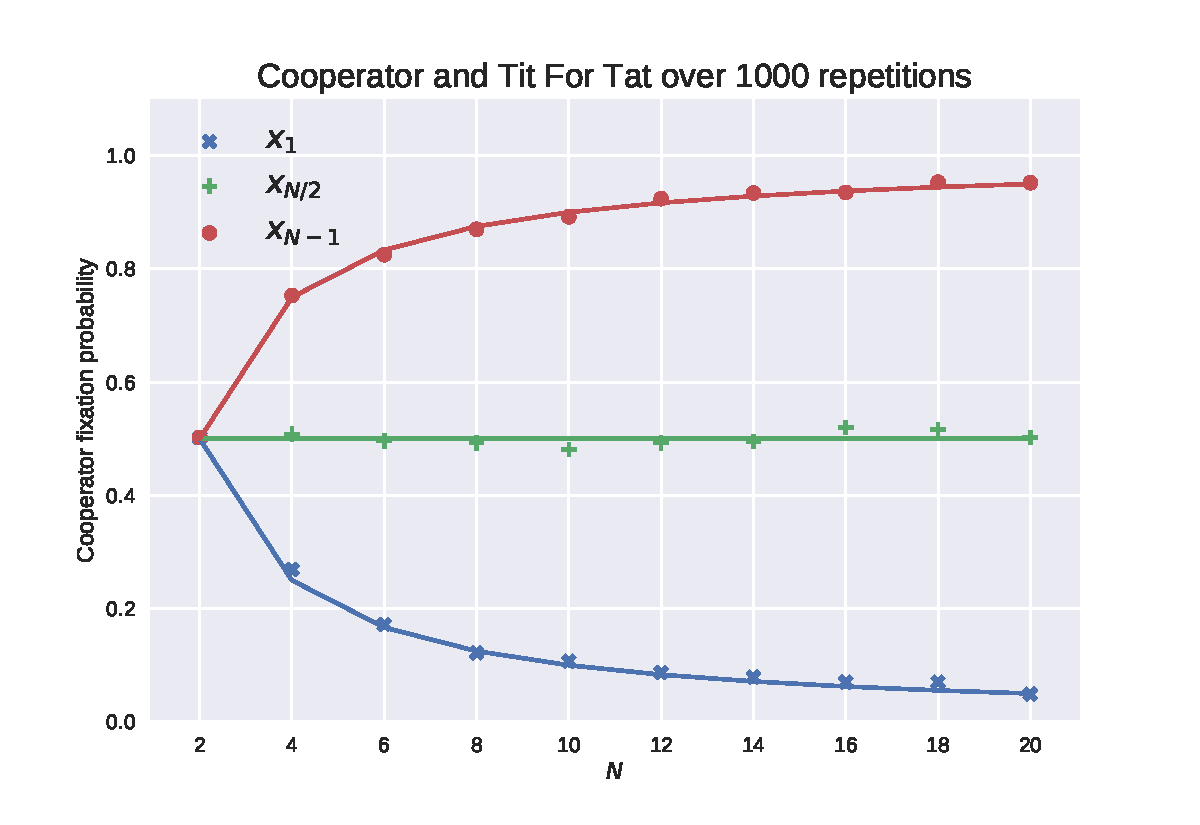
\includegraphics[width=.8\textwidth]{./img/Cooperator_v_Tit_For_Tat.pdf}
        \caption{Cooperator and Tit For Tat}
    \end{subfigure}%
    ~
    \begin{subfigure}[t]{.3\textwidth}
        \centering
        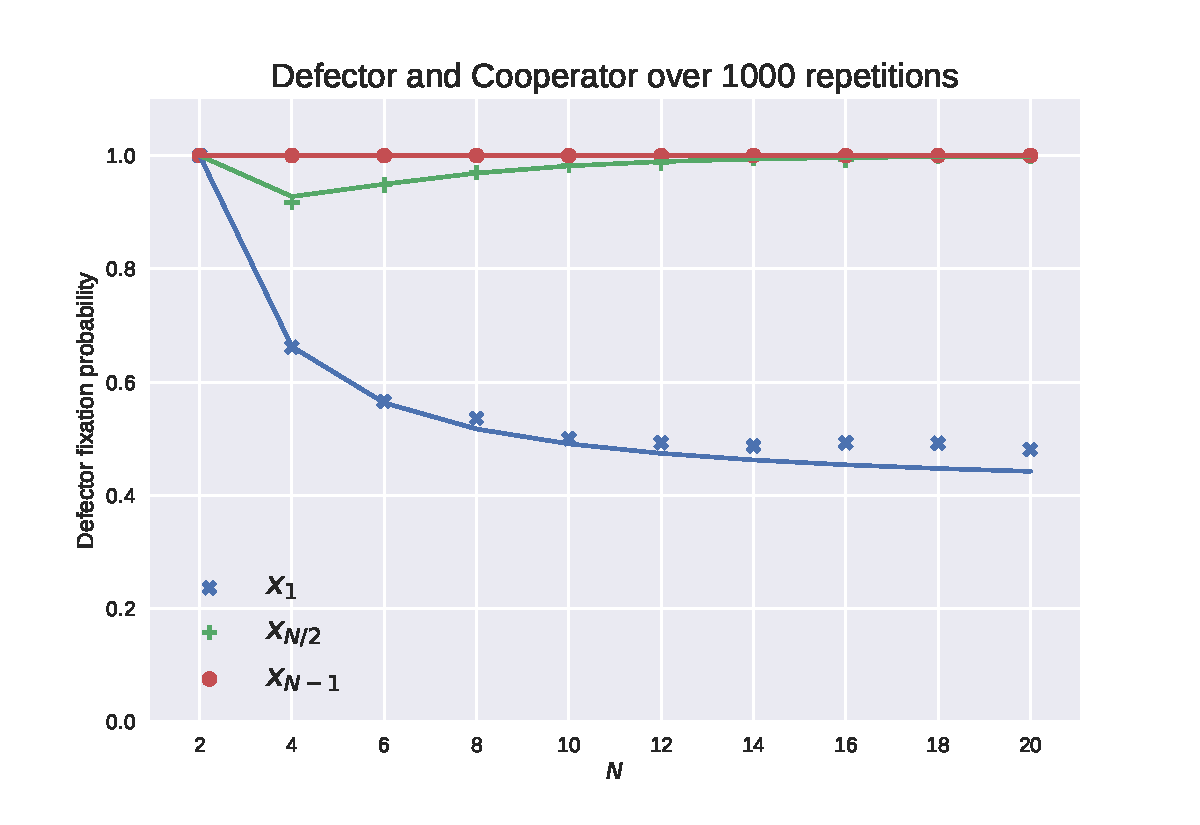
\includegraphics[width=.8\textwidth]{./img/Defector_v_Cooperator.pdf}
        \caption{Defector and Cooperator}
    \end{subfigure}%
    ~
    \begin{subfigure}[t]{.3\textwidth}
        \centering
        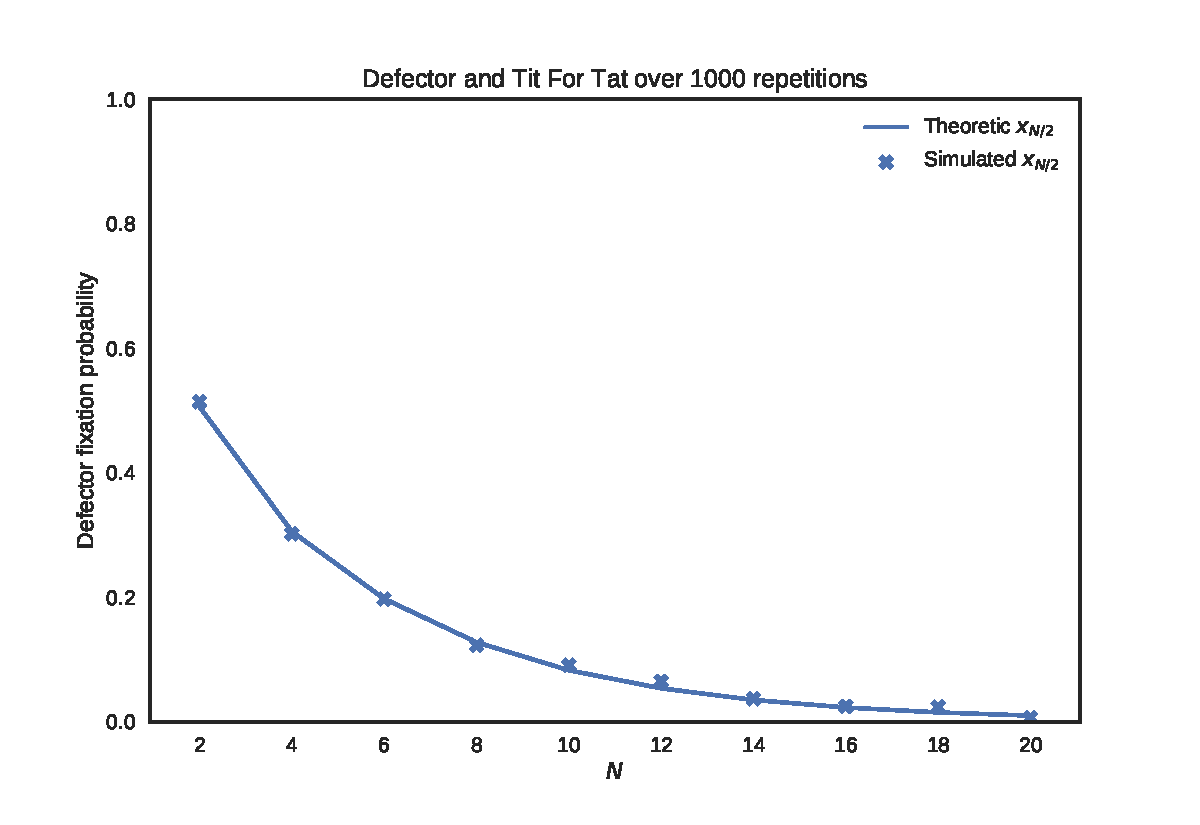
\includegraphics[width=.8\textwidth]{./img/Defector_v_Tit_For_Tat.pdf}
        \caption{Defector and Tit For Tat}
    \end{subfigure}%

    \begin{subfigure}[t]{.3\textwidth}
        \centering
        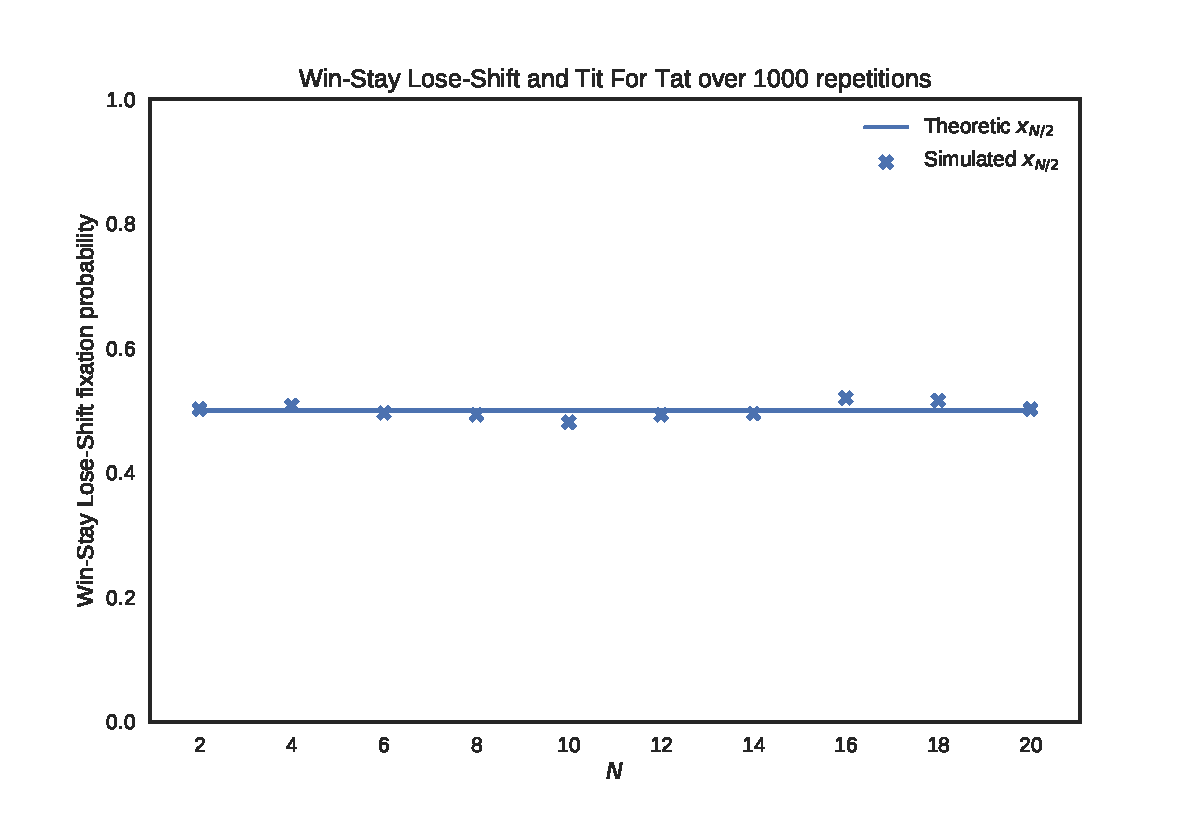
\includegraphics[width=.8\textwidth]{./img/Win-Stay_Lose-Shift_v_Tit_For_Tat.pdf}
        \caption{Win Stay Lose Shift and Tit For Tat}
    \end{subfigure}%
    ~
    \begin{subfigure}[t]{.3\textwidth}
        \centering
        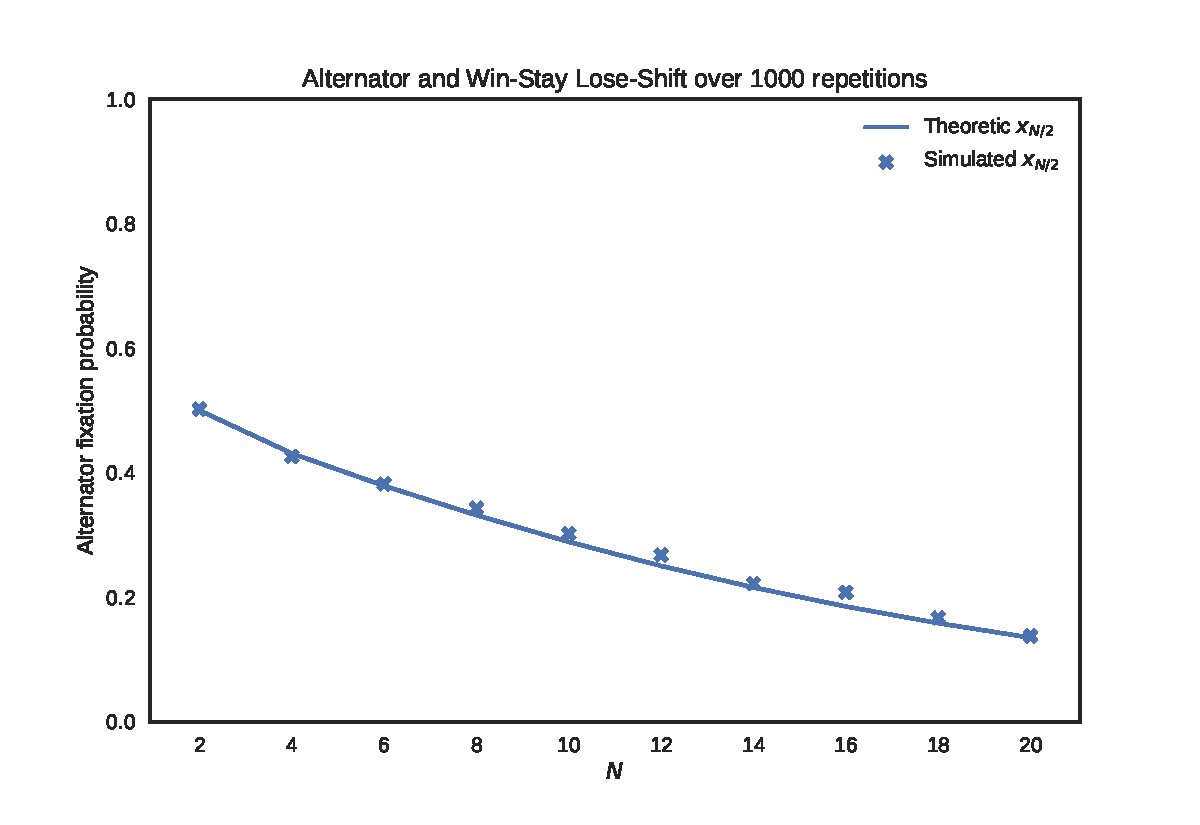
\includegraphics[width=.8\textwidth]{./img/Alternator_v_Win-Stay_Lose-Shift.pdf}
        \caption{Alternator and Win Stay Lose Shift}
    \end{subfigure}%
    ~
    \begin{subfigure}[t]{.3\textwidth}
        \centering
        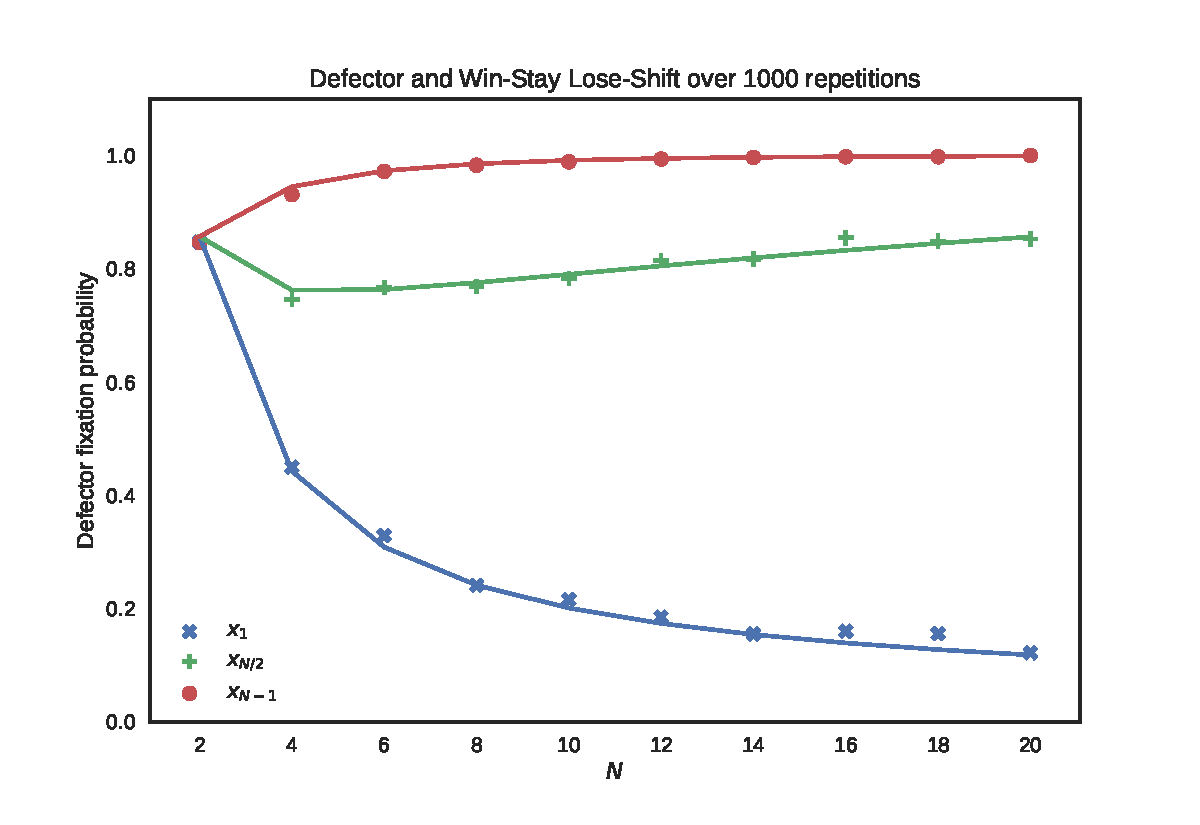
\includegraphics[width=.8\textwidth]{./img/Defector_v_Win-Stay_Lose-Shift.pdf}
        \caption{Defector and Win Stay Lose Shift}
    \end{subfigure}%
    \caption{Comparison of theoretic and actual Moran Process fixation
             probabilities for \textbf{deterministic} strategies}
    \label{fig:comparison_deterministic}
\end{figure}

\begin{figure}[!hbtp]
    \centering
    \begin{subfigure}[t]{.3\textwidth}
        \centering
        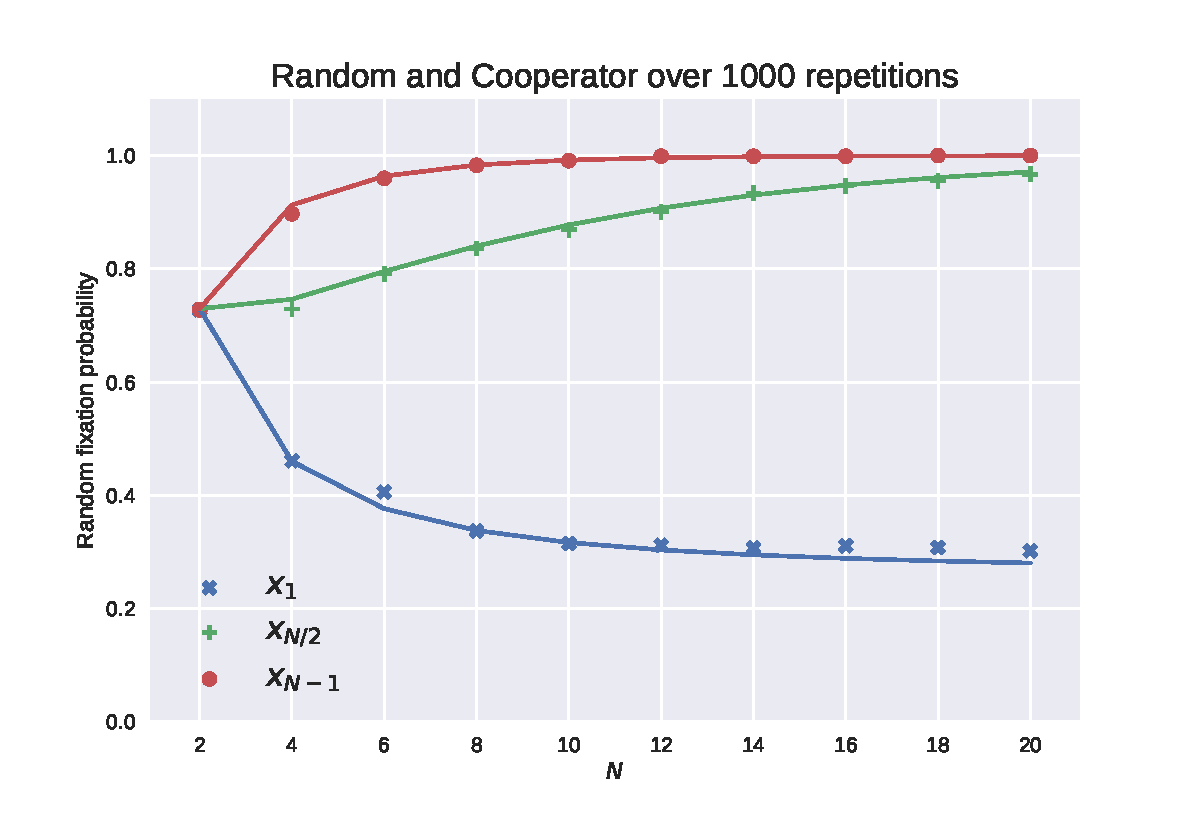
\includegraphics[width=.8\textwidth]{./img/Random_v_Cooperator.pdf}
        \caption{Random and Cooperator}
    \end{subfigure}%
    ~
    \begin{subfigure}[t]{.3\textwidth}
        \centering
        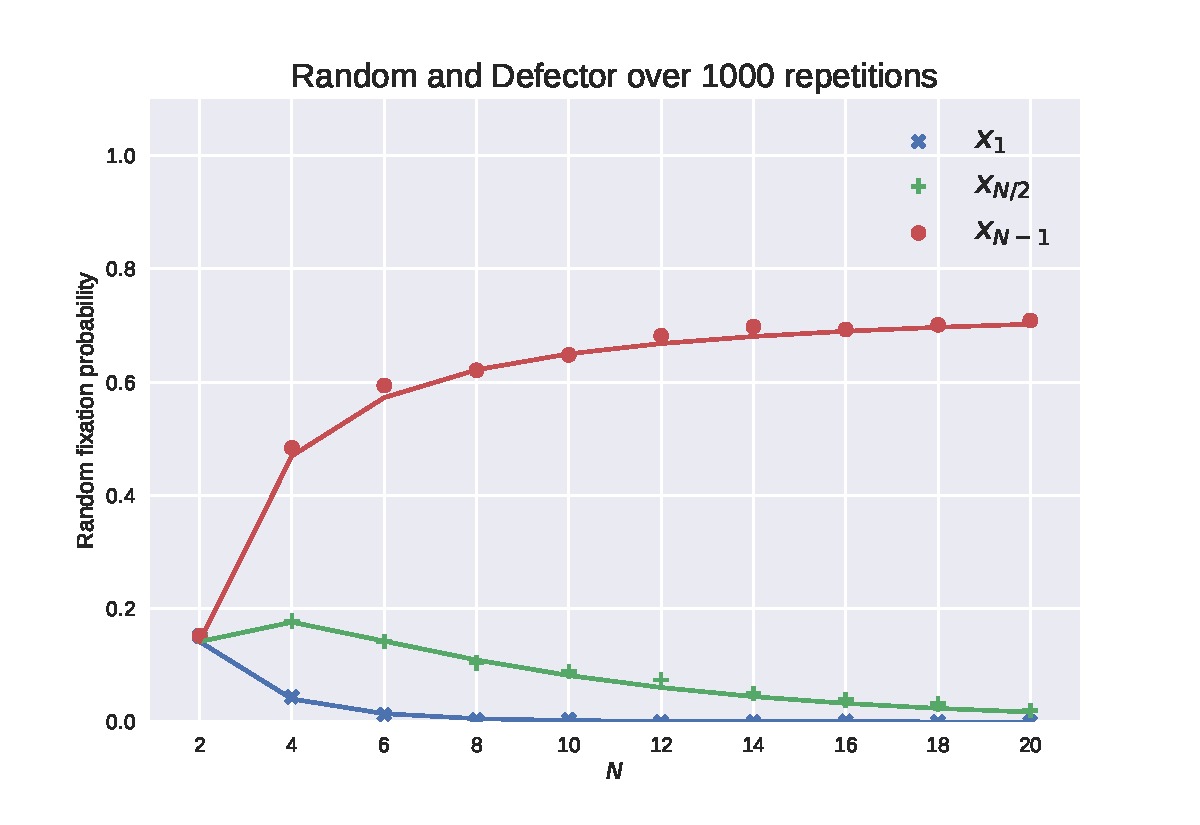
\includegraphics[width=.8\textwidth]{./img/Random_v_Defector.pdf}
        \caption{Random and Defector}
    \end{subfigure}%
    ~
    \begin{subfigure}[t]{.3\textwidth}
        \centering
        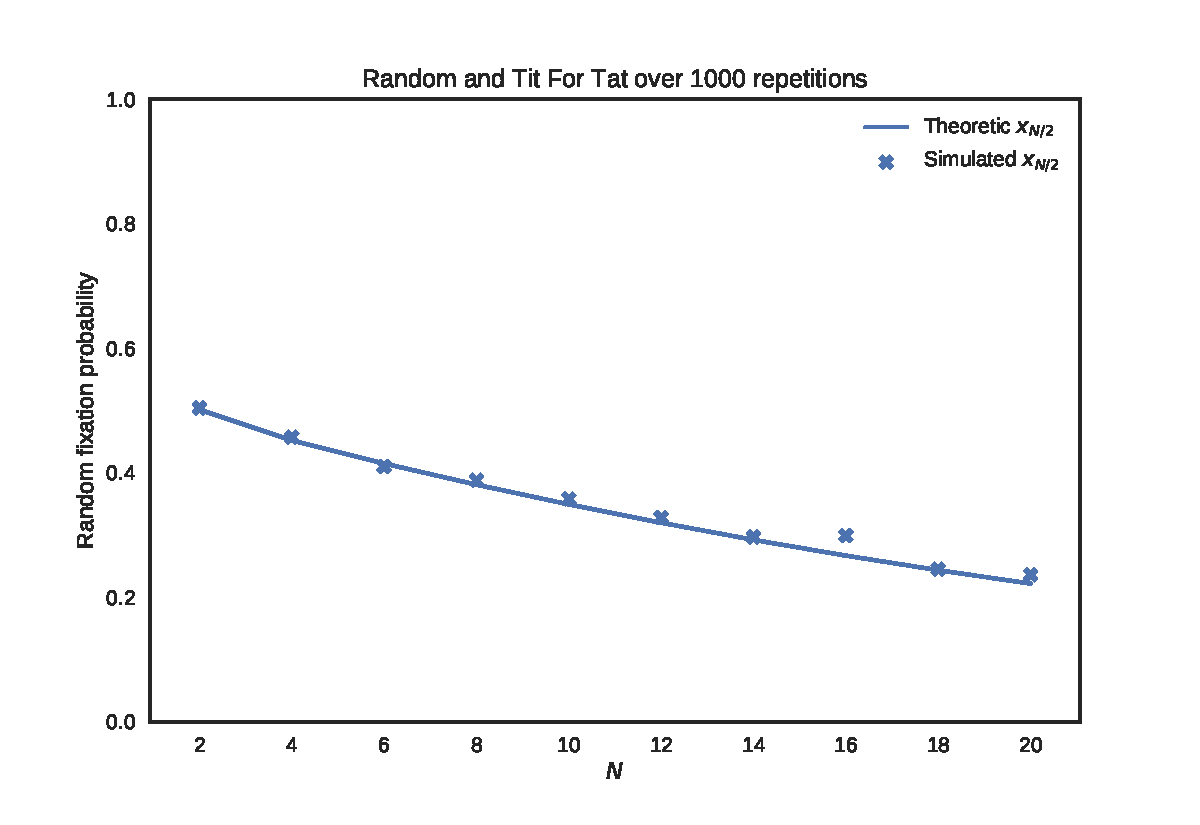
\includegraphics[width=.8\textwidth]{./img/Random_v_Tit_For_Tat.pdf}
        \caption{Random and Tit For Tat}
    \end{subfigure}%

    \begin{subfigure}[t]{.3\textwidth}
        \centering
        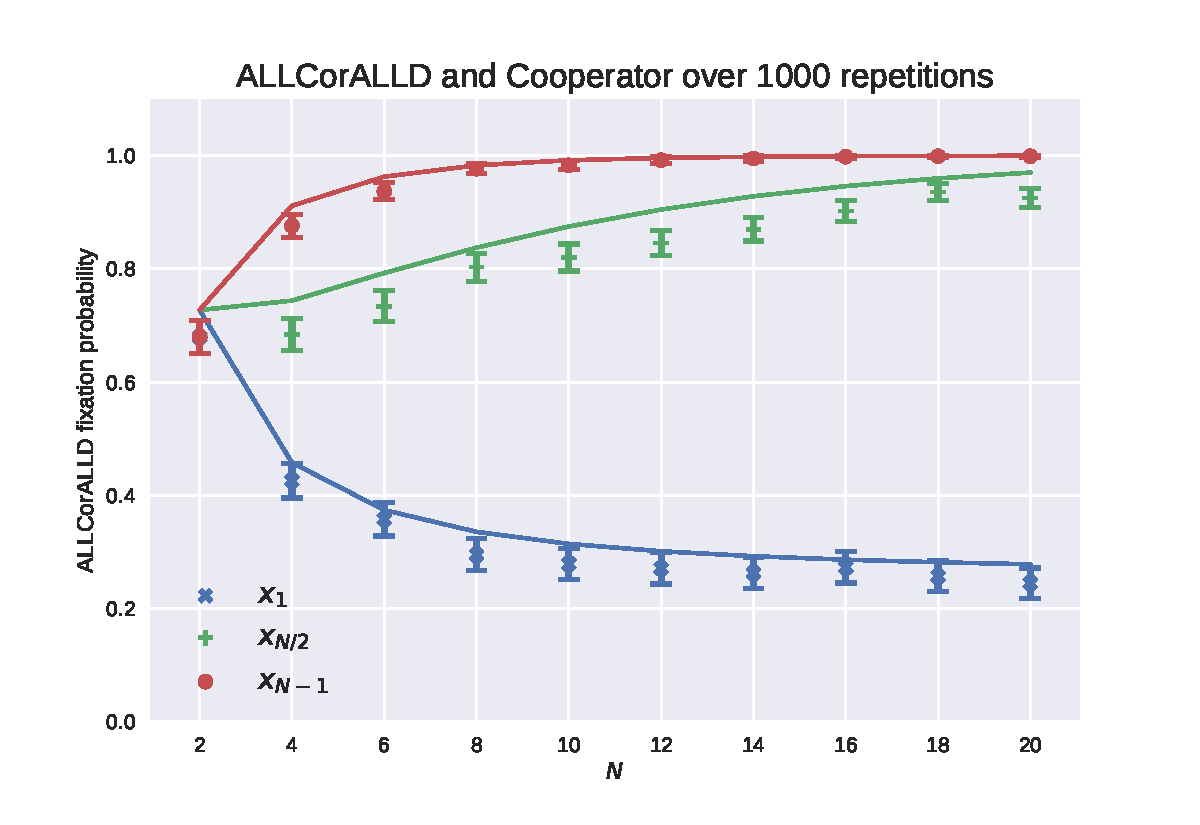
\includegraphics[width=.8\textwidth]{./img/ALLCorALLD_v_Cooperator.pdf}
        \caption{All C or all D and Cooperator}
    \end{subfigure}%
    ~
    \begin{subfigure}[t]{.3\textwidth}
        \centering
        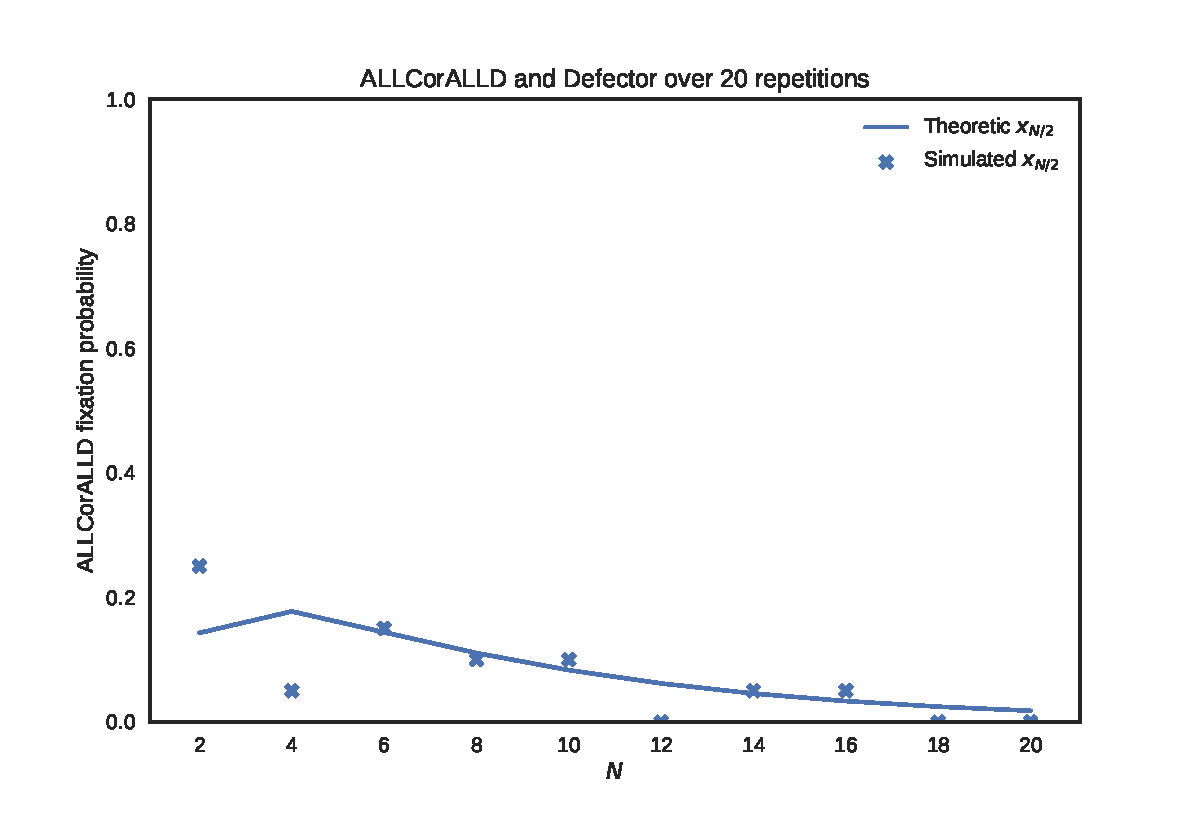
\includegraphics[width=.8\textwidth]{./img/ALLCorALLD_v_Defector.pdf}
        \caption{All C or all D and Defector}
    \end{subfigure}%
    ~
    \begin{subfigure}[t]{.3\textwidth}
        \centering
        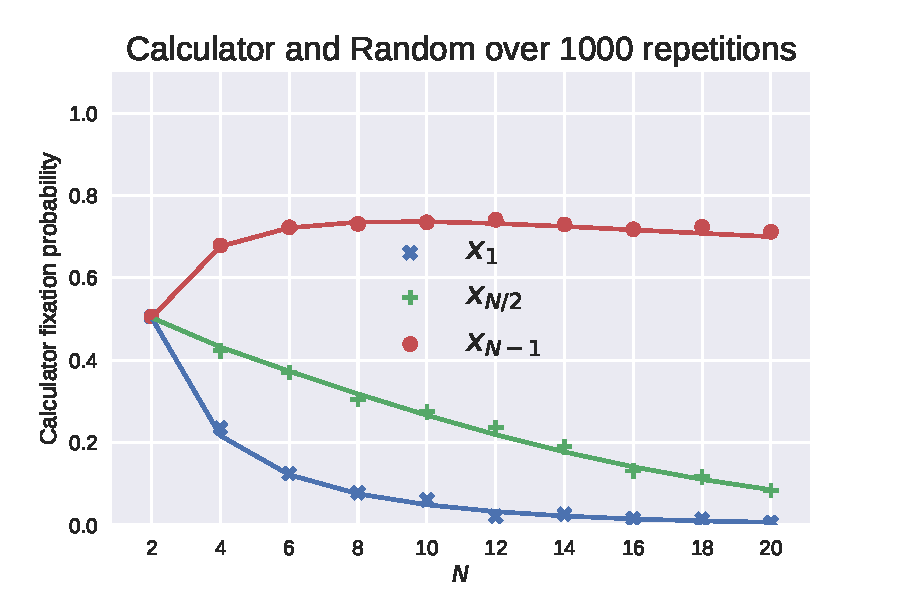
\includegraphics[width=.8\textwidth]{./img/Calculator_v_Random.pdf}
        \caption{Calculator and Random}
    \end{subfigure}%

    \begin{subfigure}[t]{.3\textwidth}
        \centering
        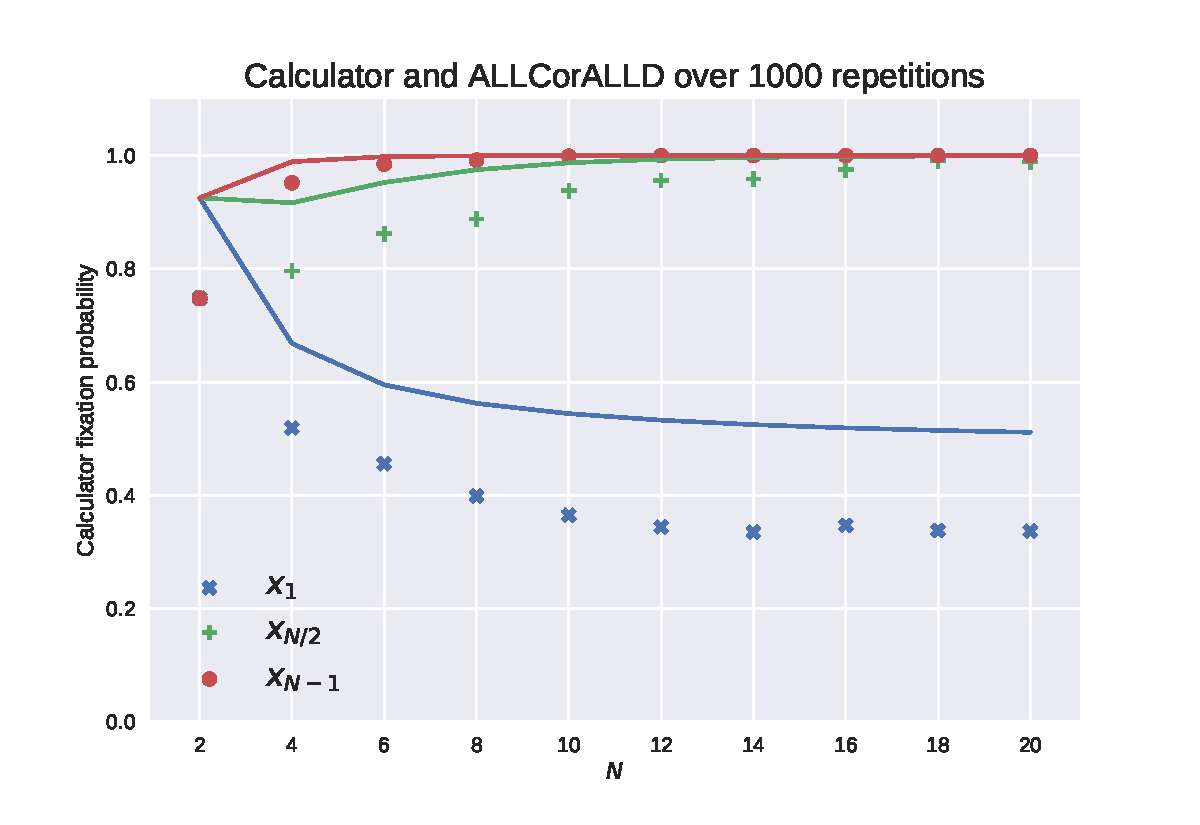
\includegraphics[width=.8\textwidth]{./img/Calculator_v_ALLCorALLD.pdf}
        \caption{Calculator and All C or all D}
    \end{subfigure}%
    ~
    \begin{subfigure}[t]{.3\textwidth}
        \centering
        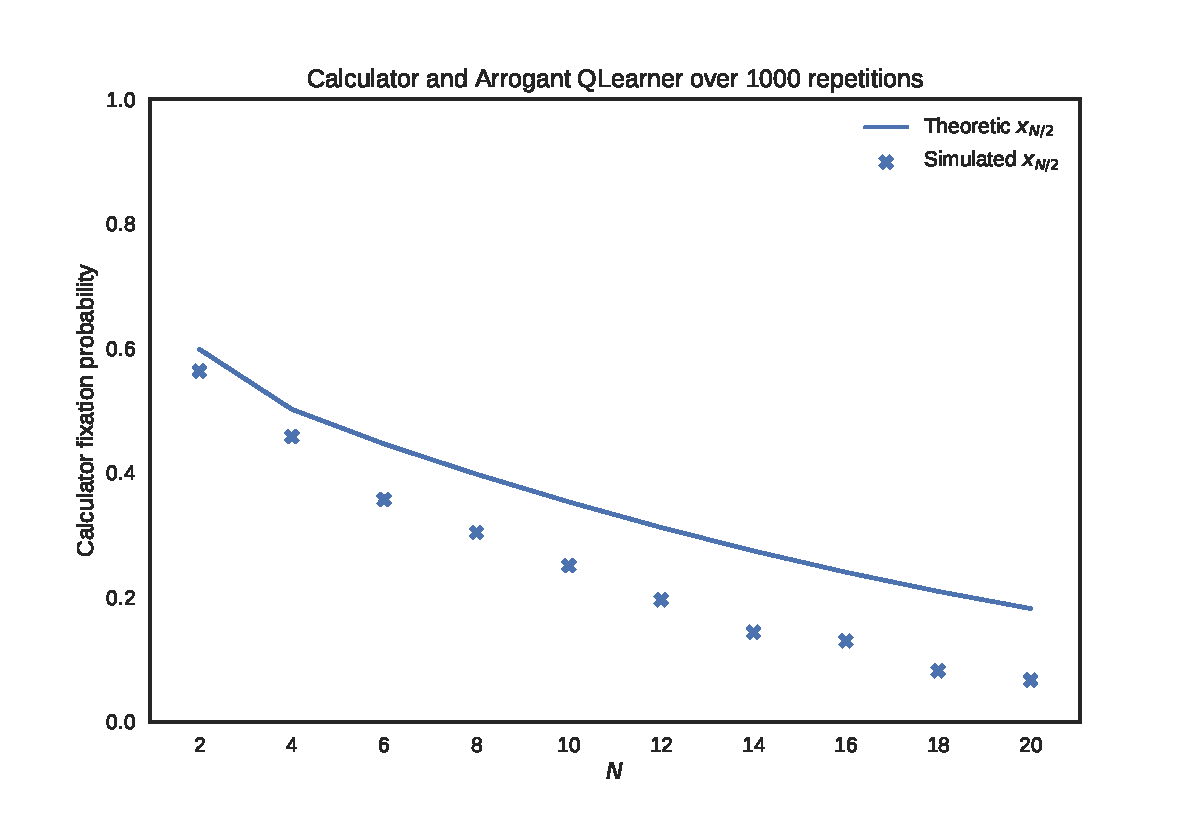
\includegraphics[width=.8\textwidth]{./img/Calculator_v_Arrogant_QLearner.pdf}
        \caption{Calculator and Arrogant Q learner}
    \end{subfigure}%
    ~
    \begin{subfigure}[t]{.3\textwidth}
        \centering
        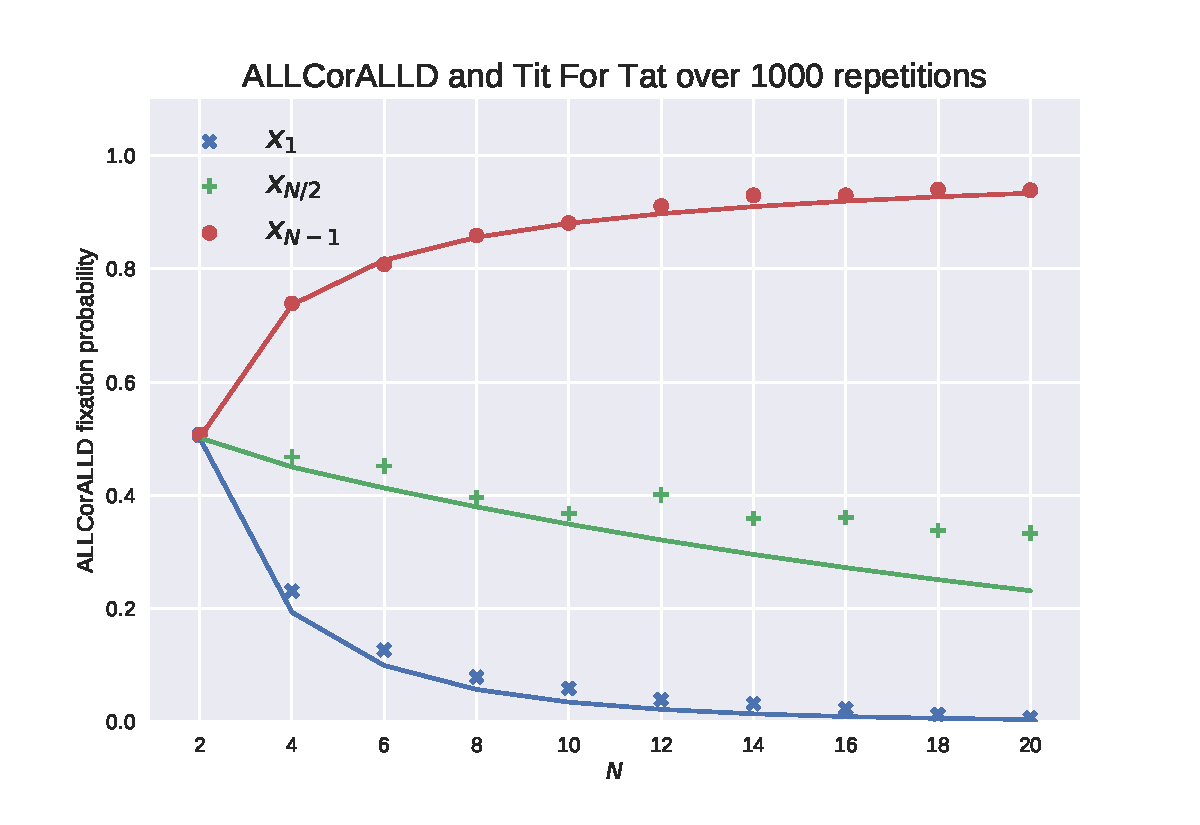
\includegraphics[width=.8\textwidth]{./img/ALLCorALLD_v_Tit_For_Tat.pdf}
        \caption{All C or all D and Tit For Tat}
    \end{subfigure}%
    \caption{Comparison of theoretic and actual Moran Process
             fixation probabilities for \textbf{stochastic} strategies}
    \label{fig:comparison_stochastic}
\end{figure}

Figure~\ref{fig:comparison_stochastic} shows the fixation probabilities for
stochastic strategies. These are no longer a good match which highlights the
weakness of the analytical formulae that relies on the average payoffs. A
detailed analysis of the 164 strategies considered, using direct Moran processes
will be shown in the next Section.

\section{Empirical results}\label{sec:empirical_results}

% TODO Archive all data (Zenodo) and include details/reference here.

This section will outline the data analysis carried out:

\begin{itemize}
    \item Section~\ref{sec:two_individuals} will consider the specific case of
        \(N=2\).
    \item Section~\ref{sec:strong_invaders} will investigate the effect of
        population size on the ability of a strategy to invade another
        population. This will highlight how complex strategies with long
        memories outperform simpler strategies.
    \item Section~\ref{sec:strong_resistors} will similarly investigate the
        ability to defend against an invasion.
    \item Section~\ref{sec:population_size} will investigate the relationship
        between performance for differing population sizes. This highlights the
        importance of considering population dynamics over large populations.
    \item Section~\ref{sec:relative_fitness} will calculate the relative fitness of all
        strategies.
\end{itemize}

\subsection{The special case of \(N=2\)}\label{sec:two_individuals}

The main fixation probabilities of interest are \(x_1\) and \(x_{N-1}\), these
reflect a strategy's ability to invade or resist invasion.
% TODO Perhaps mention that a lot of the research in to training fixation of
% strategies assumes N=2? Is this true?
For \(N=2\) these two cases coincide. Figure~\ref{fig:fixation_heatmap_2} shows
all pairwise fixation probabilities for strategies on the vertical column when
being matched against probabilities on the horizontal column. This is summarised
in Figure~\ref{fig:boxplot_2} and Table~\ref{tbl:summary_top_2}.

\begin{enumerate}
    \item The top strategy is an extortionate Zero determinant
        strategy~\cite{Press2012} with parameters \(l=1\) and \(s=1/4\).
    \item The Collective strategy has a simple handshake mechanism (a
        cooperation followed by a defection on the first move). As long as the
        opponent plays the same handshake and does not defect in the future it
        cooperates. Otherwise it defects for all rounds~\cite{Li2009}.  This
        strategy was specifically designed for Evolutionary processes so it is
        perhaps also not surprising that it does well here.
    \item The finite state machine strategy % TODO Perhaps refer to earlier
        % discussion in the methodology section about these FSM strategies
    \item The Feld strategy is the corresponding strategy submitted to Axelrod's
        first tournament~\cite{Axelrod1980a}: it punishes defections but
        otherwise defects with a random probability that decays over time.
    \item The final strategy in the top five is another extortionate Zero
        determinant strategy~\cite{Press2012} with parameters \(l=p\).
\end{enumerate}


\begin{figure}[!hbtp]
    \begin{subfigure}[t]{.4\textwidth}
        \centering
        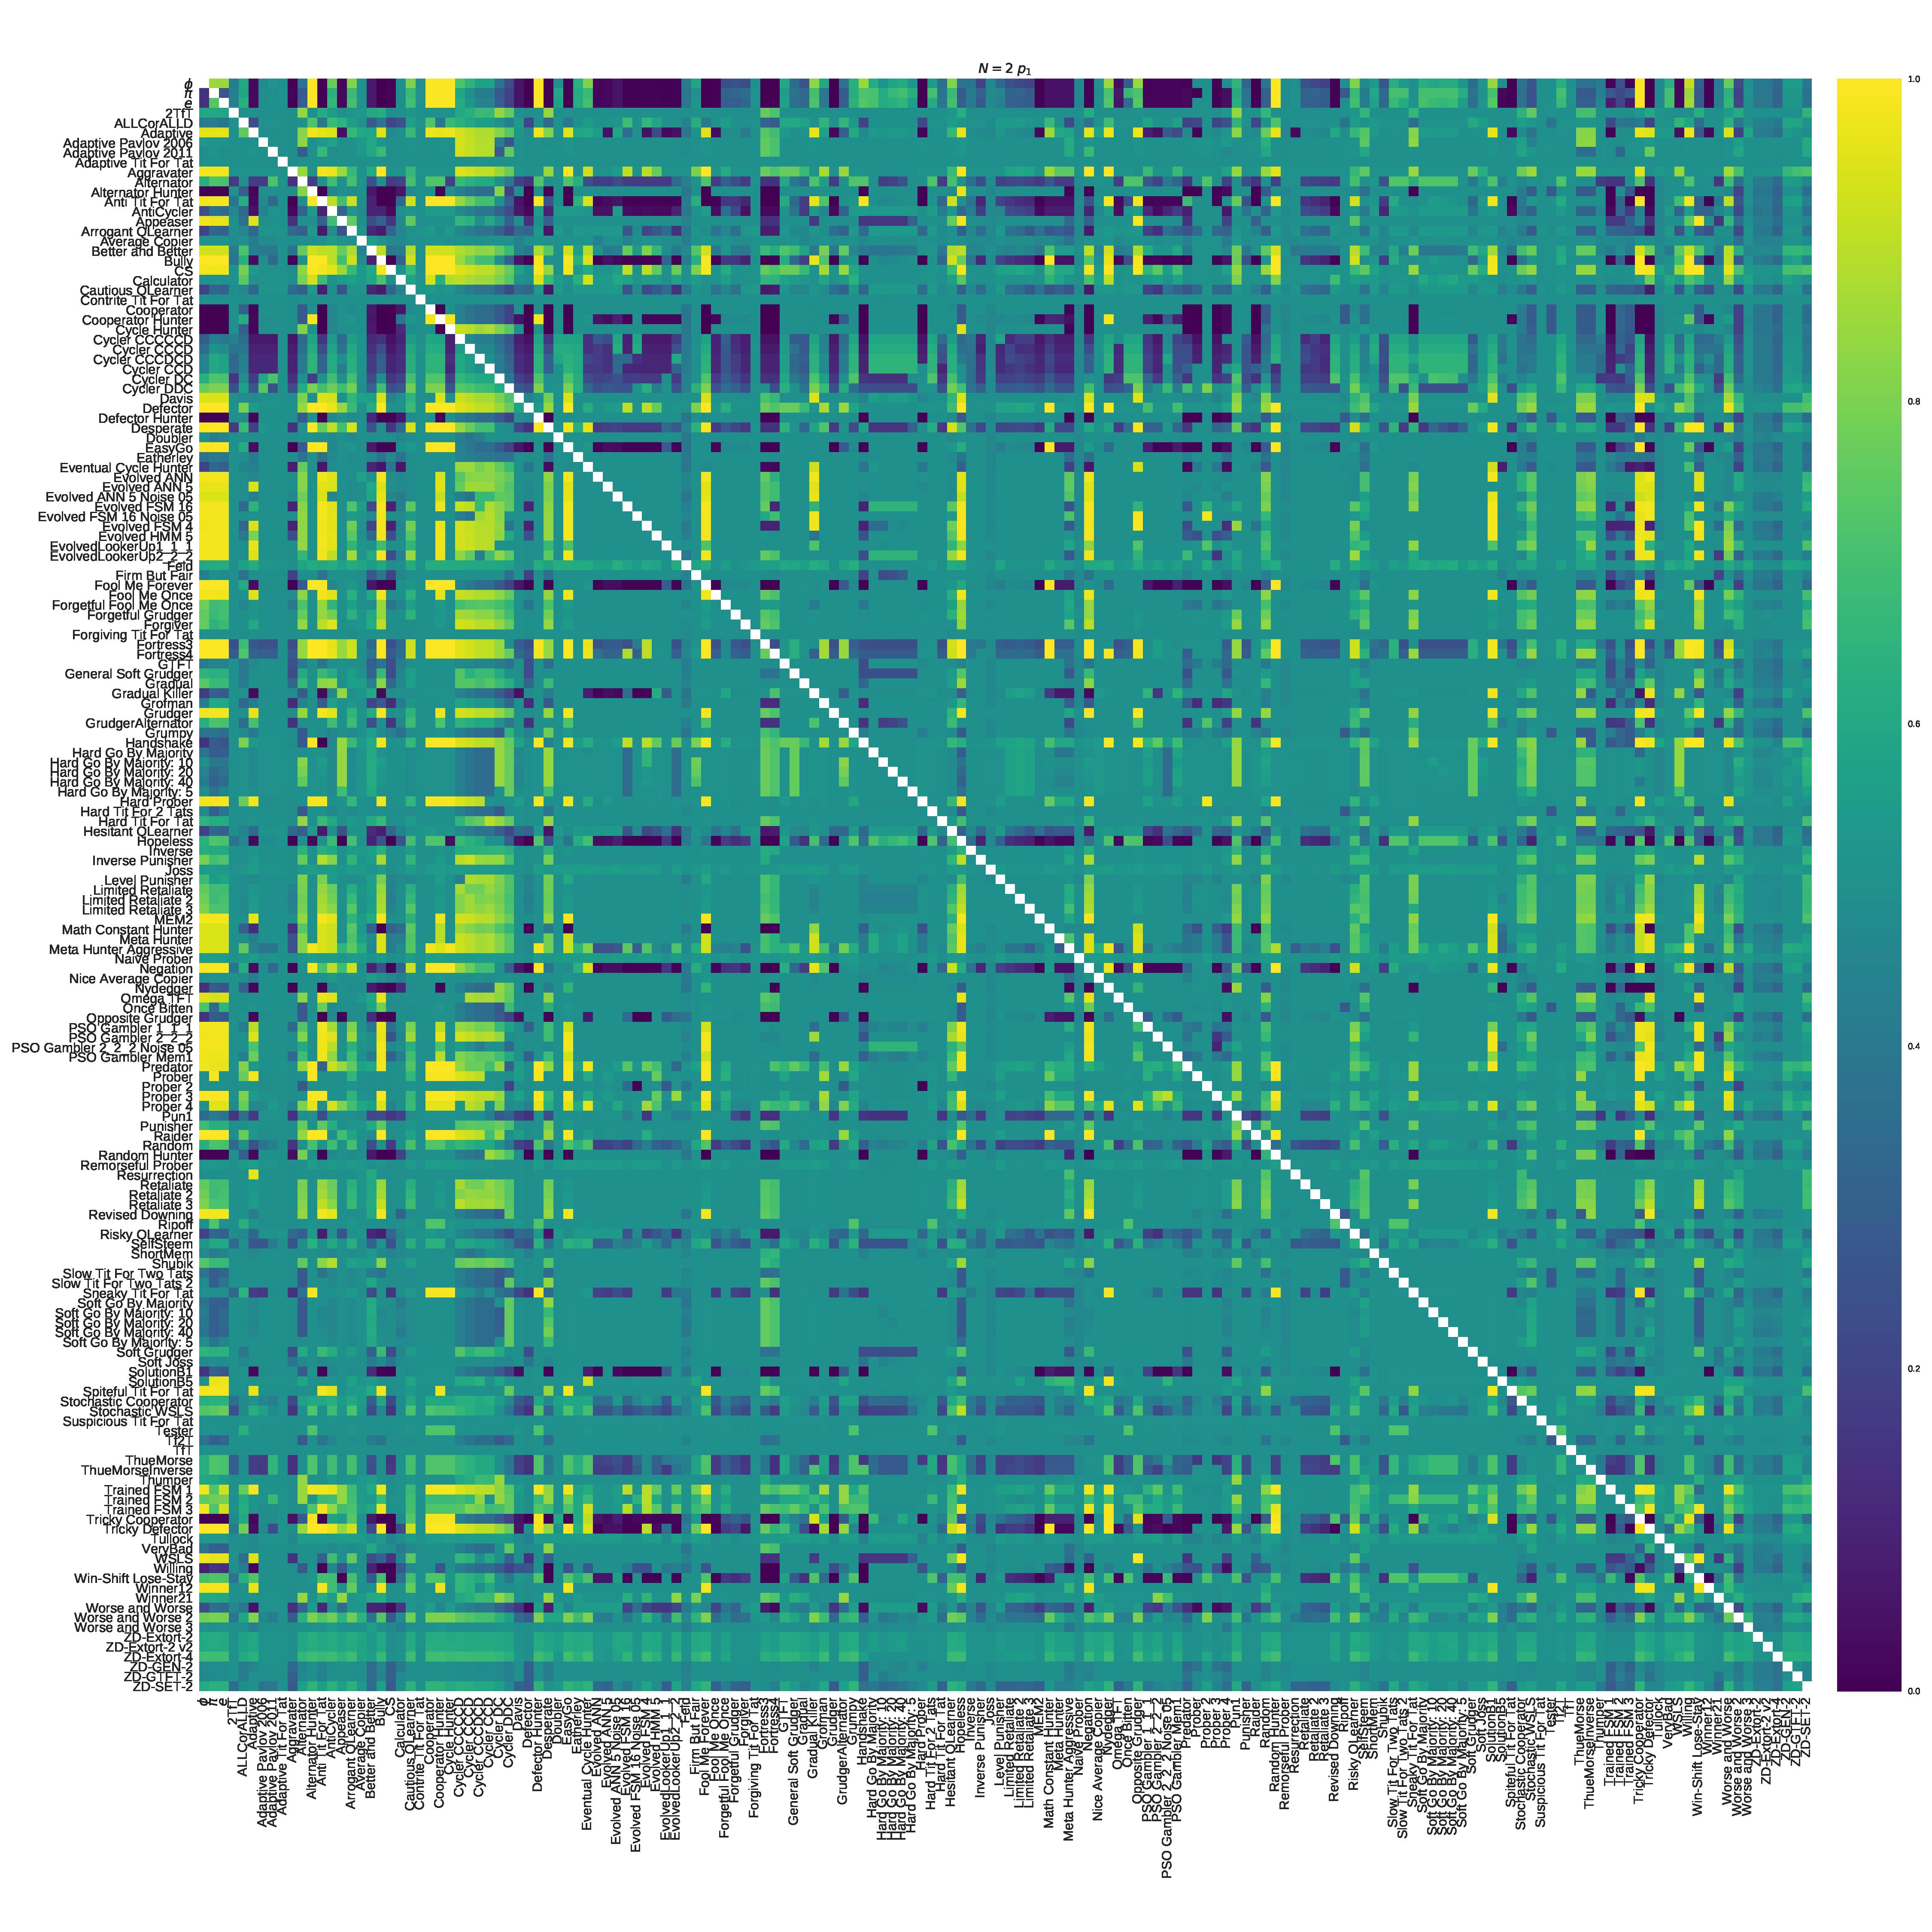
\includegraphics[width=\textwidth]{./img/fixation_heatmap_2_invade.pdf}
        % TODO Remove this: I don't feel it is effective.
        \caption{The pairwise fixation probabilities for \(N=2\)}
        \label{fig:fixation_heatmap_2}
    \end{subfigure}%
    ~
    \begin{subfigure}[t]{.6\textwidth}
        \centering
        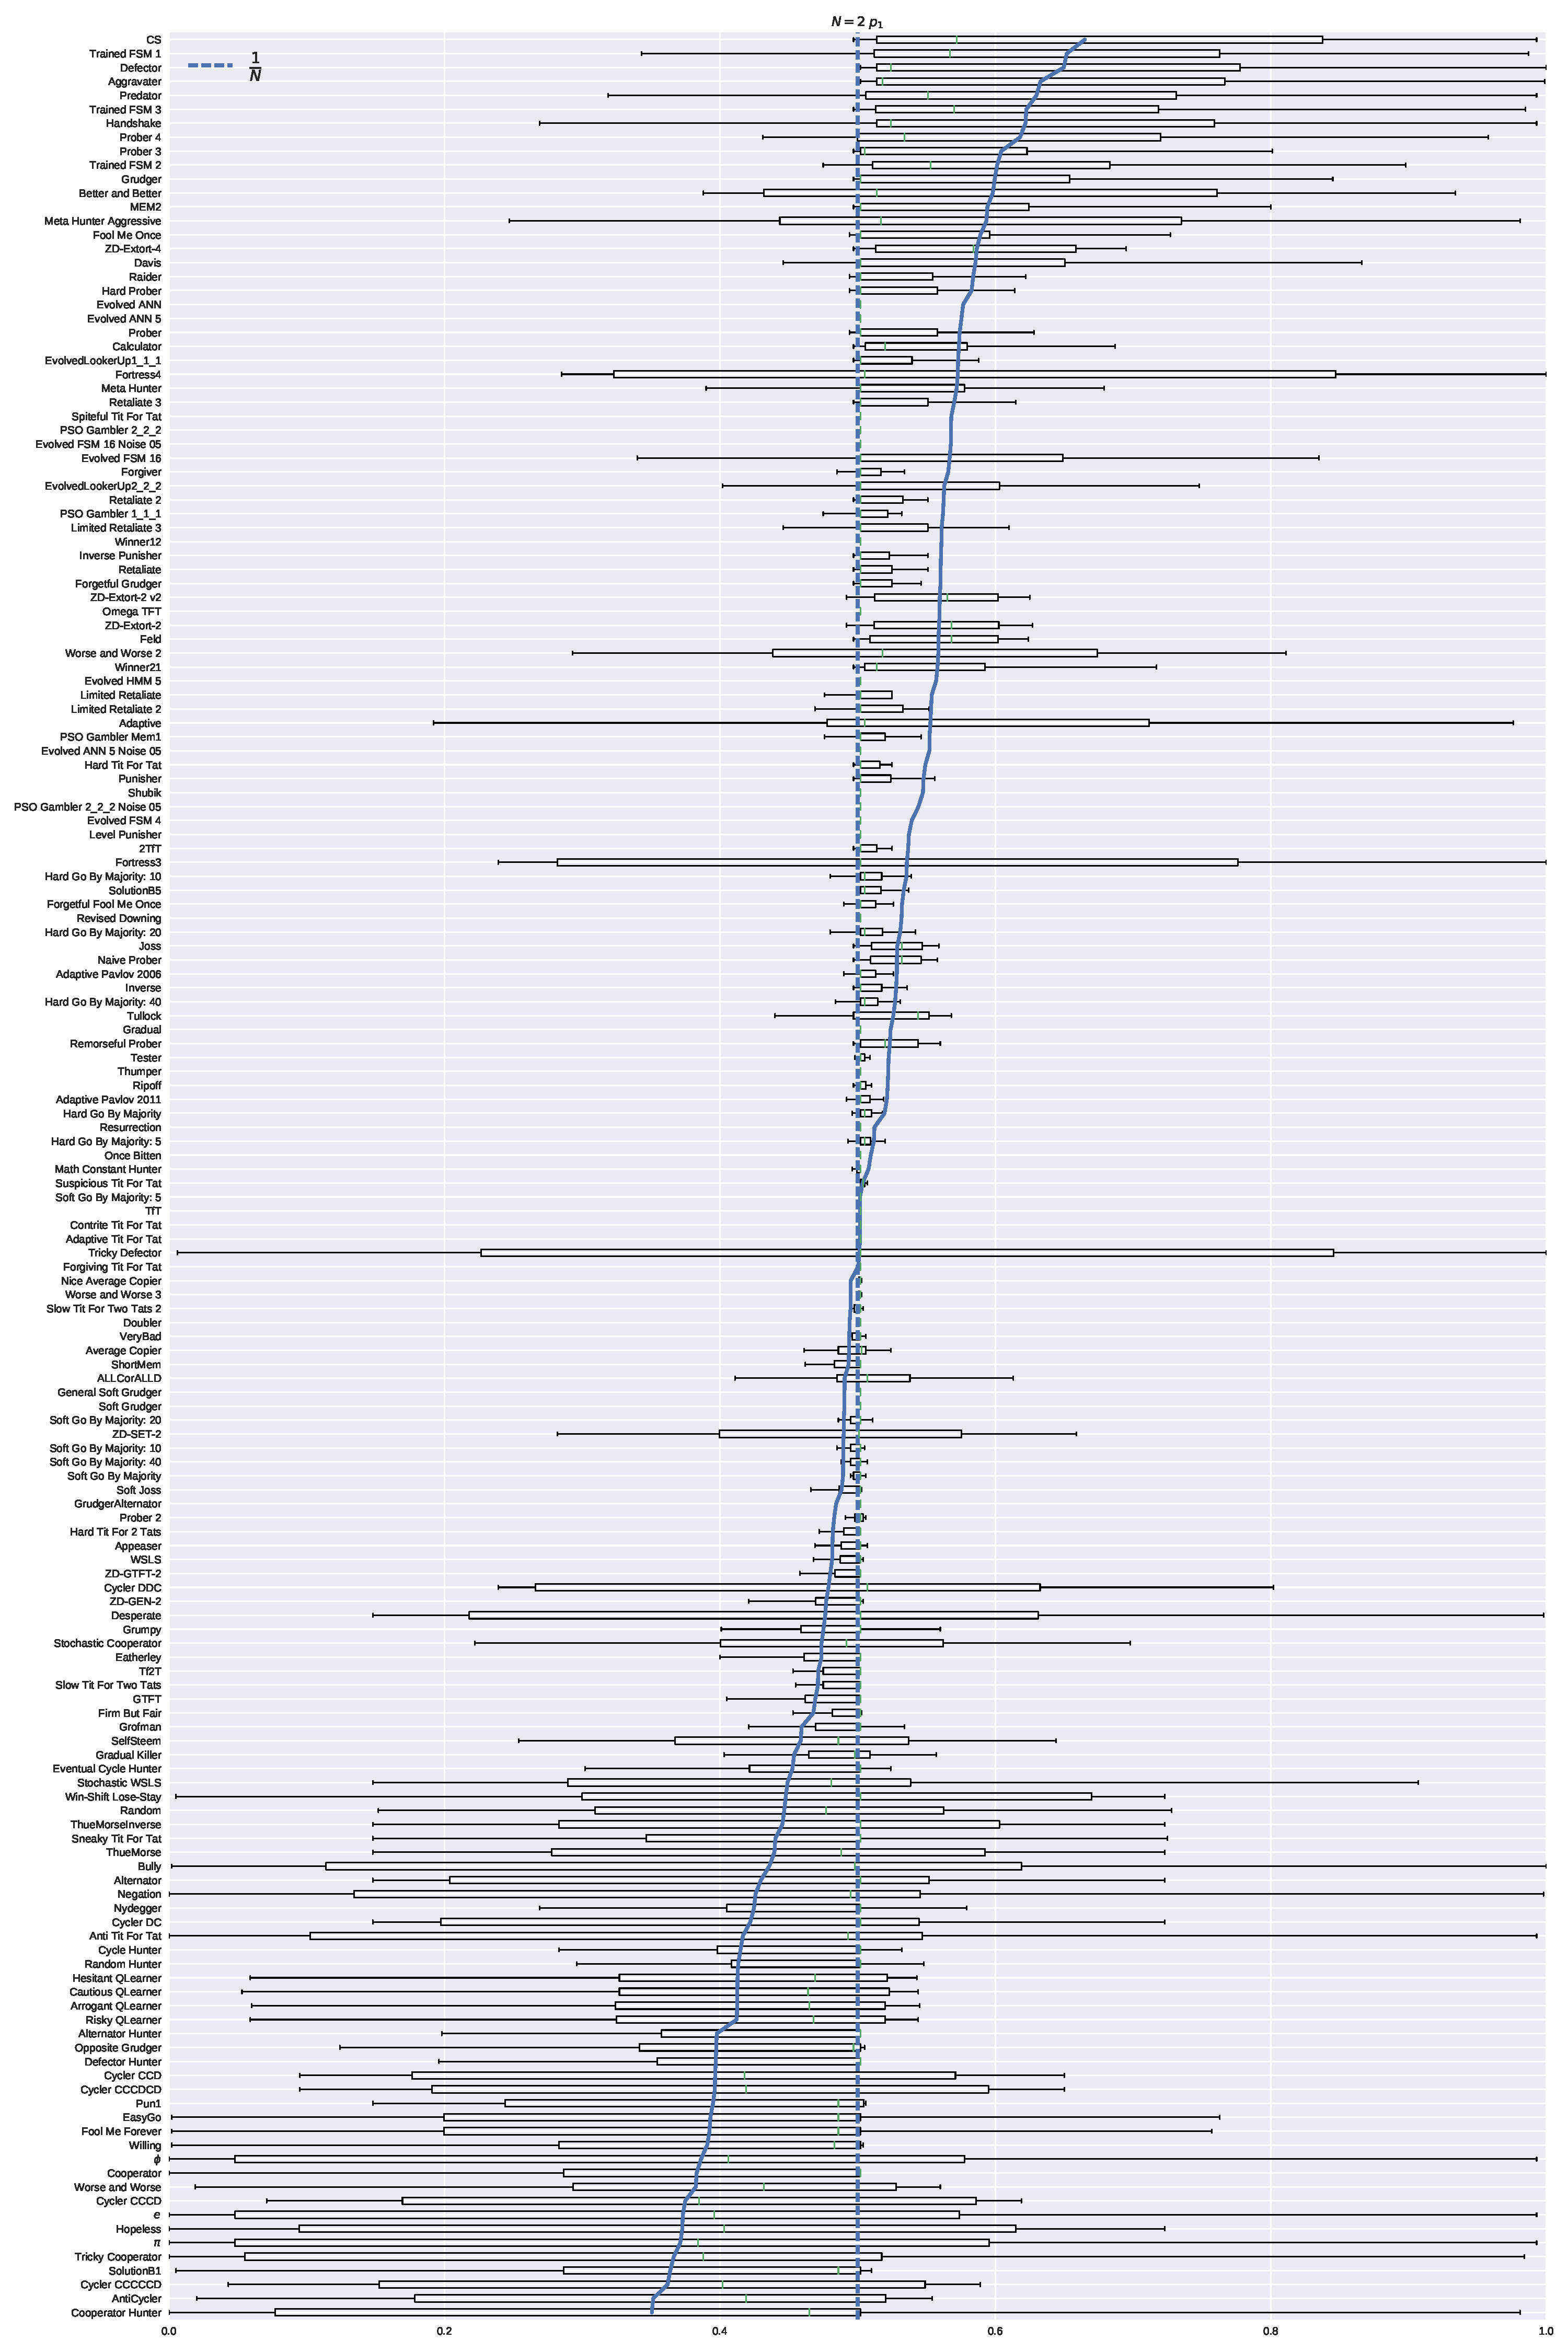
\includegraphics[height=.8\textheight]{./img/boxplot_2_invade.pdf}
        \caption{The median fixation probabilities for \(N=2\)}
        \label{fig:boxplot_2}
    \end{subfigure}
\end{figure}

\begin{table}[!hbtp]
    \centering
    \begin{tabular}{lrrl}
\toprule
        Player &  Median $p_1$ &  Memory Depth & Stochastic \\
\midrule
   ZD-Extort-4 &         0.584 &             1 &       True \\
            CS &         0.572 &            \(\infty\) &      False \\
 Trained FSM 3 &         0.570 &             1 &      False \\
          Feld &         0.568 &           200 &       True \\
   ZD-Extort-2 &         0.568 &             1 &       True \\
\bottomrule
\end{tabular}

    \caption{Summary of top five strategies for \(N=2\)}
    \label{tbl:summary_top_2}
\end{table}

As will be demonstrated in Section~\ref{sec:population_size} \(N=2\)
is a particular case. In the next sections we will pay close attention to
strategies who are strong invaders/resistors and shown diagrammatically in
Figure~\ref{fig:invasion_resistance}.

\begin{figure}[!hbtp]
    \centering
    \documentclass{standalone}
\usepackage{tikz}
\usetikzlibrary{calc, shapes, patterns}

\begin{document}
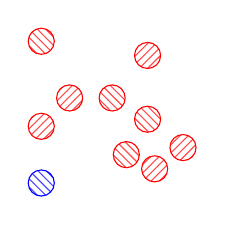
\begin{tikzpicture}[scale=.9]
	\node (A1) at (-1, -1) [circle, pattern=north west lines, pattern
        color=blue!70, draw=blue] {};
	\node (A2) at (-1, 1) [circle, pattern=north west lines, pattern
        color=red!70, draw=red] {};
	\node (A3) at (0, .2) [circle, pattern=north west lines, pattern
        color=red!70, draw=red] {};
	\node (A4) at (.2, -.6) [circle, pattern=north west lines, pattern
        color=red!70, draw=red] {};
	\node (A5) at (.5, -0.1) [circle, pattern=north west lines, pattern
        color=red!70, draw=red] {};
	\node (B1) at (-1, -.2) [circle, pattern=north east lines, pattern
        color=red!70, draw=red] {};
	\node (B2) at (1, -.5) [circle, pattern=north east lines, pattern
        color=red!70, draw=red] {};
	\node (B3) at (.5, .8) [circle, pattern=north east lines, pattern
        color=red!70, draw=red] {};
	\node (B4) at (-.6, .2) [circle, pattern=north east lines, pattern
        color=red!70, draw=red] {};
	\node (B5) at (.6, -.8) [circle, pattern=north east lines, pattern
        color=red!70, draw=red] {};
\end{tikzpicture}
\end{document}

    \caption{A single individual will successfully invade the population with
    probability \(x_1\). The group of Individuals will successfully resist with
    probability \(x_{N-1}\)}
    \label{fig:invasion_resistance}
\end{figure}

\subsection{Strong invaders}\label{sec:strong_invaders}

In this section \(x_i\) will be investigated: the probability of 1 individual of
a given type successfully becoming fixated in a population of \(N - 1\) other
individuals. Figures~\ref{fig:fixation_heatmap_invade} shows these values for
the players along the vertical axis when matched against the players on the
horizontal axis. It can be seen that invasion is in general more challenging for
\(N=7\) and \(N=12\) in comparison to \(N=3\).
%TODO Change this to N=14
This information is summarised in Figure~\ref{fig:fixation_boxplot_invade}
showing the median fixation as well as the neutral fixation for each given
scenario.

\begin{figure}[!hbtp]
    \centering
    \begin{subfigure}[t]{.3\textwidth}
        \centering
        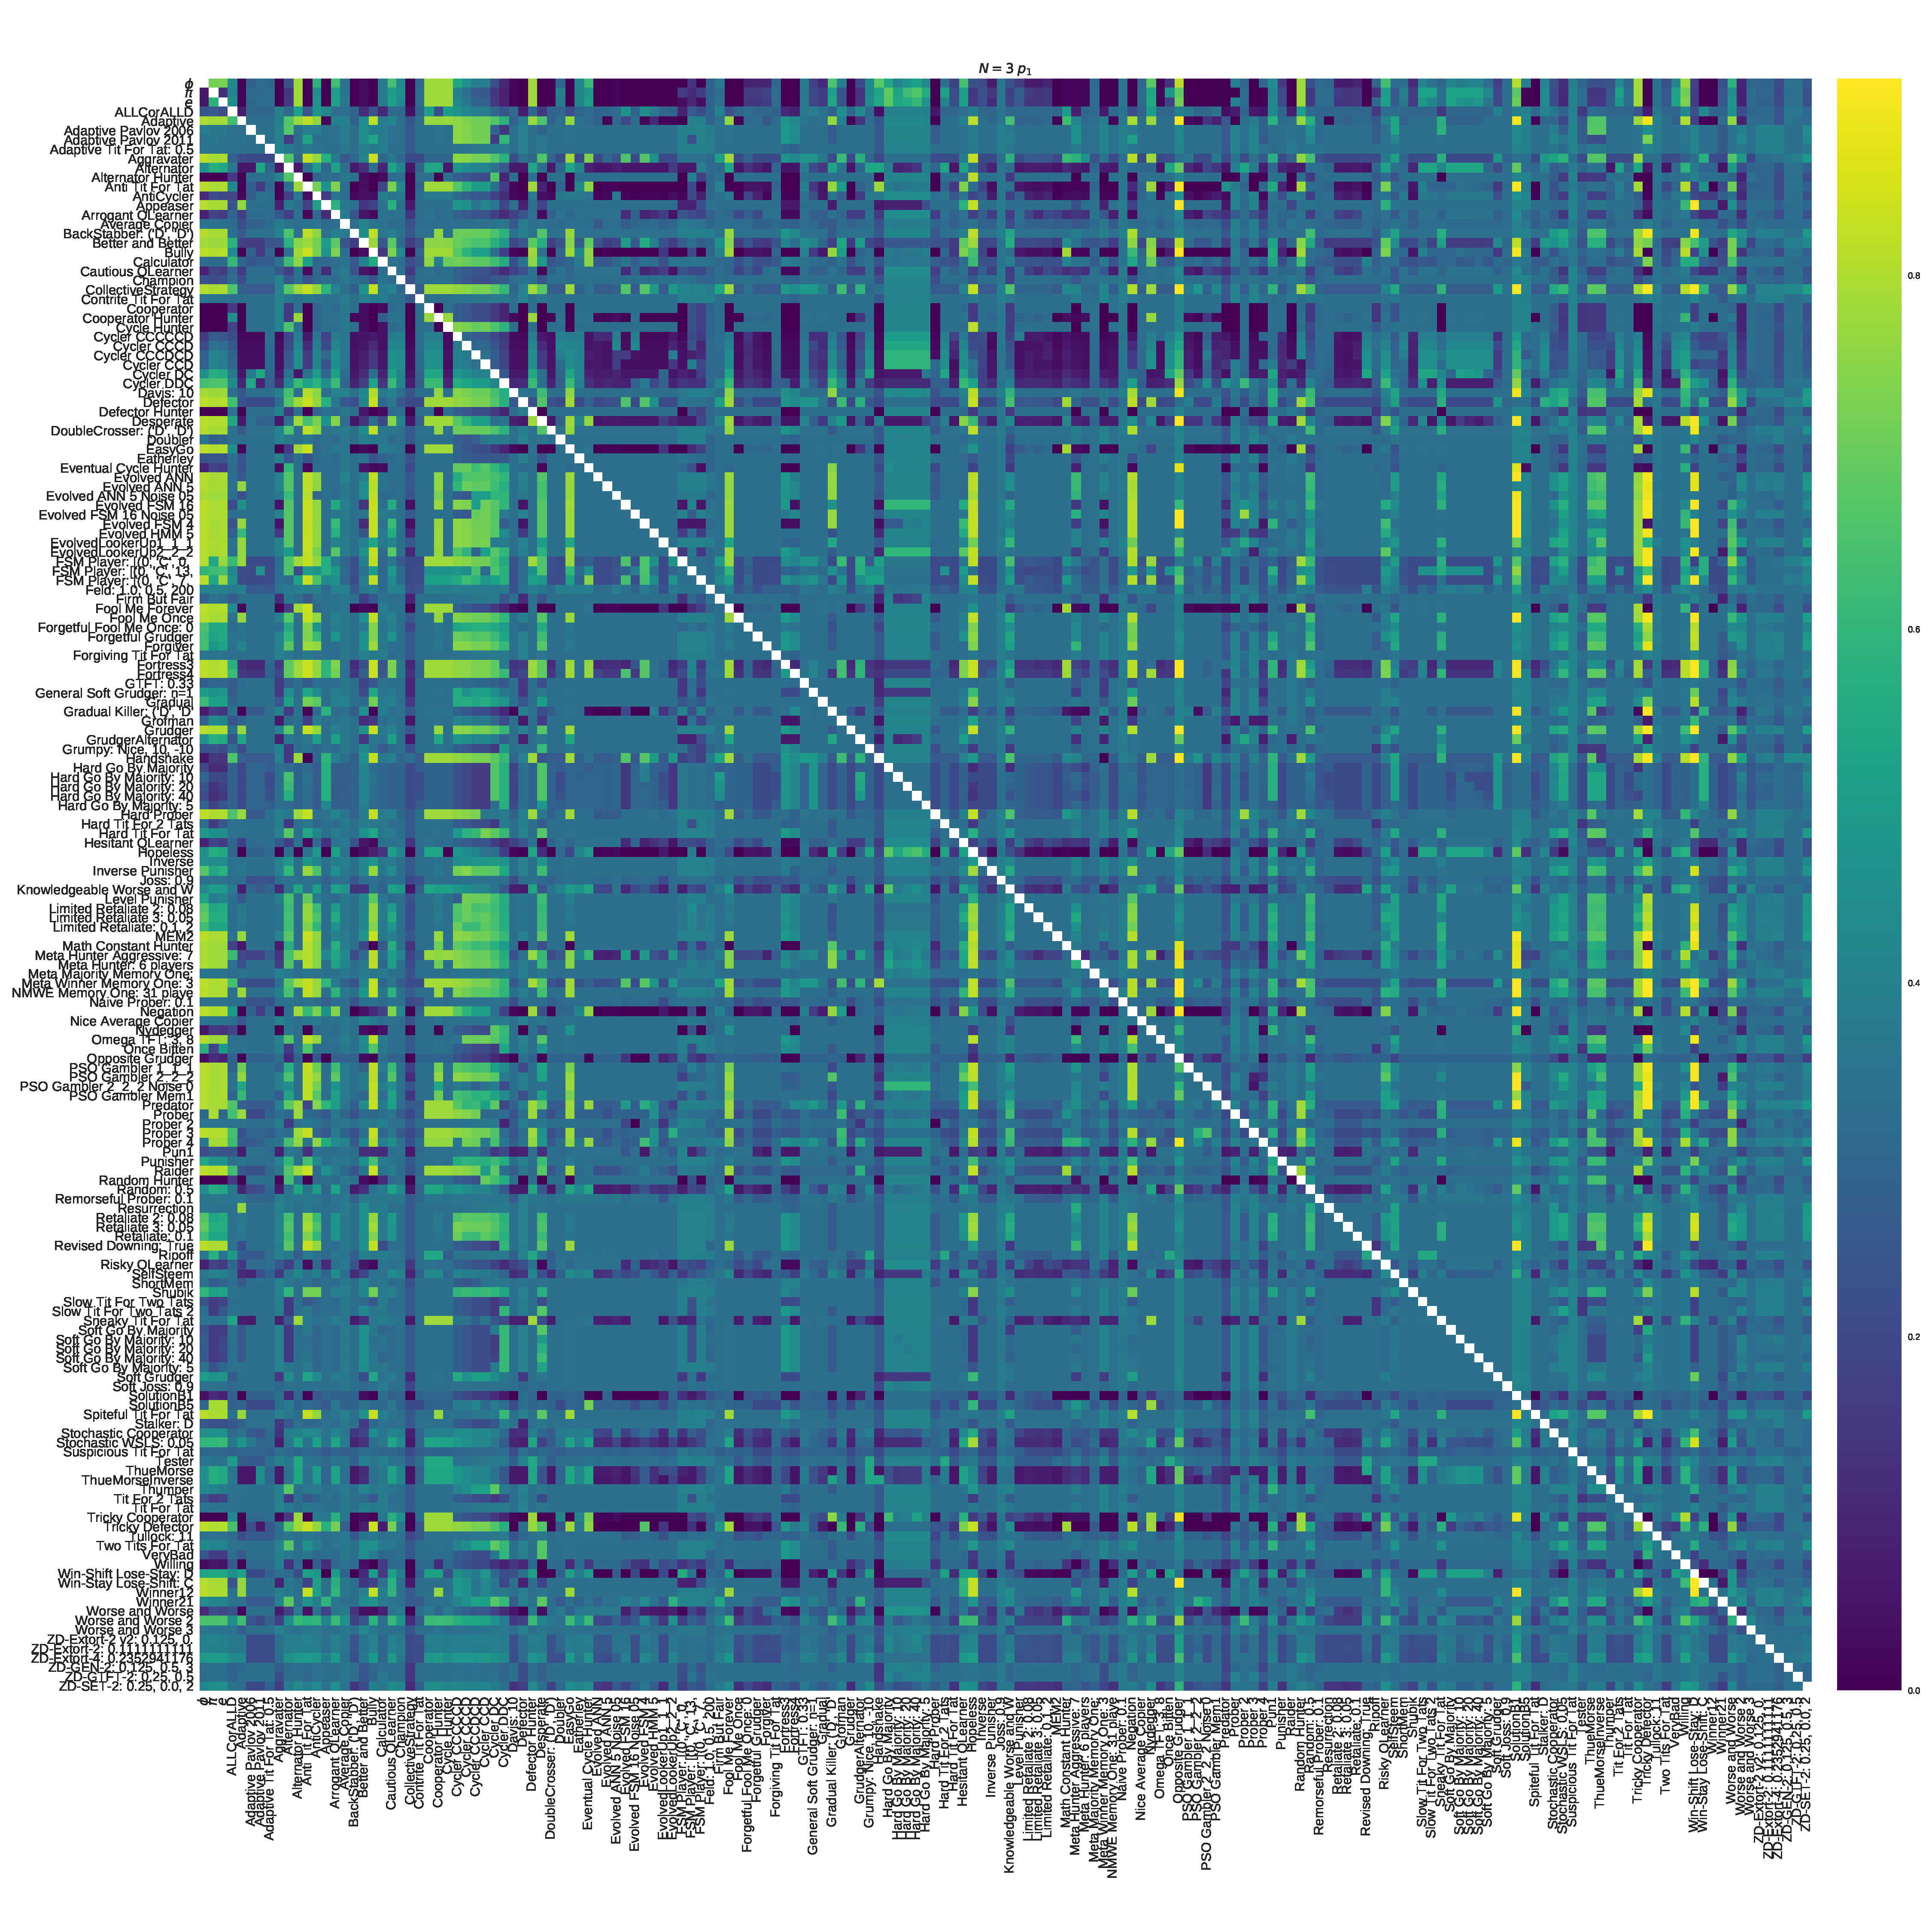
\includegraphics[width=.8\textwidth]{./img/fixation_heatmap_3_invade.pdf}
        \caption{\(N=3\)}
    \end{subfigure}%
    ~
    \begin{subfigure}[t]{.3\textwidth}
        \centering
        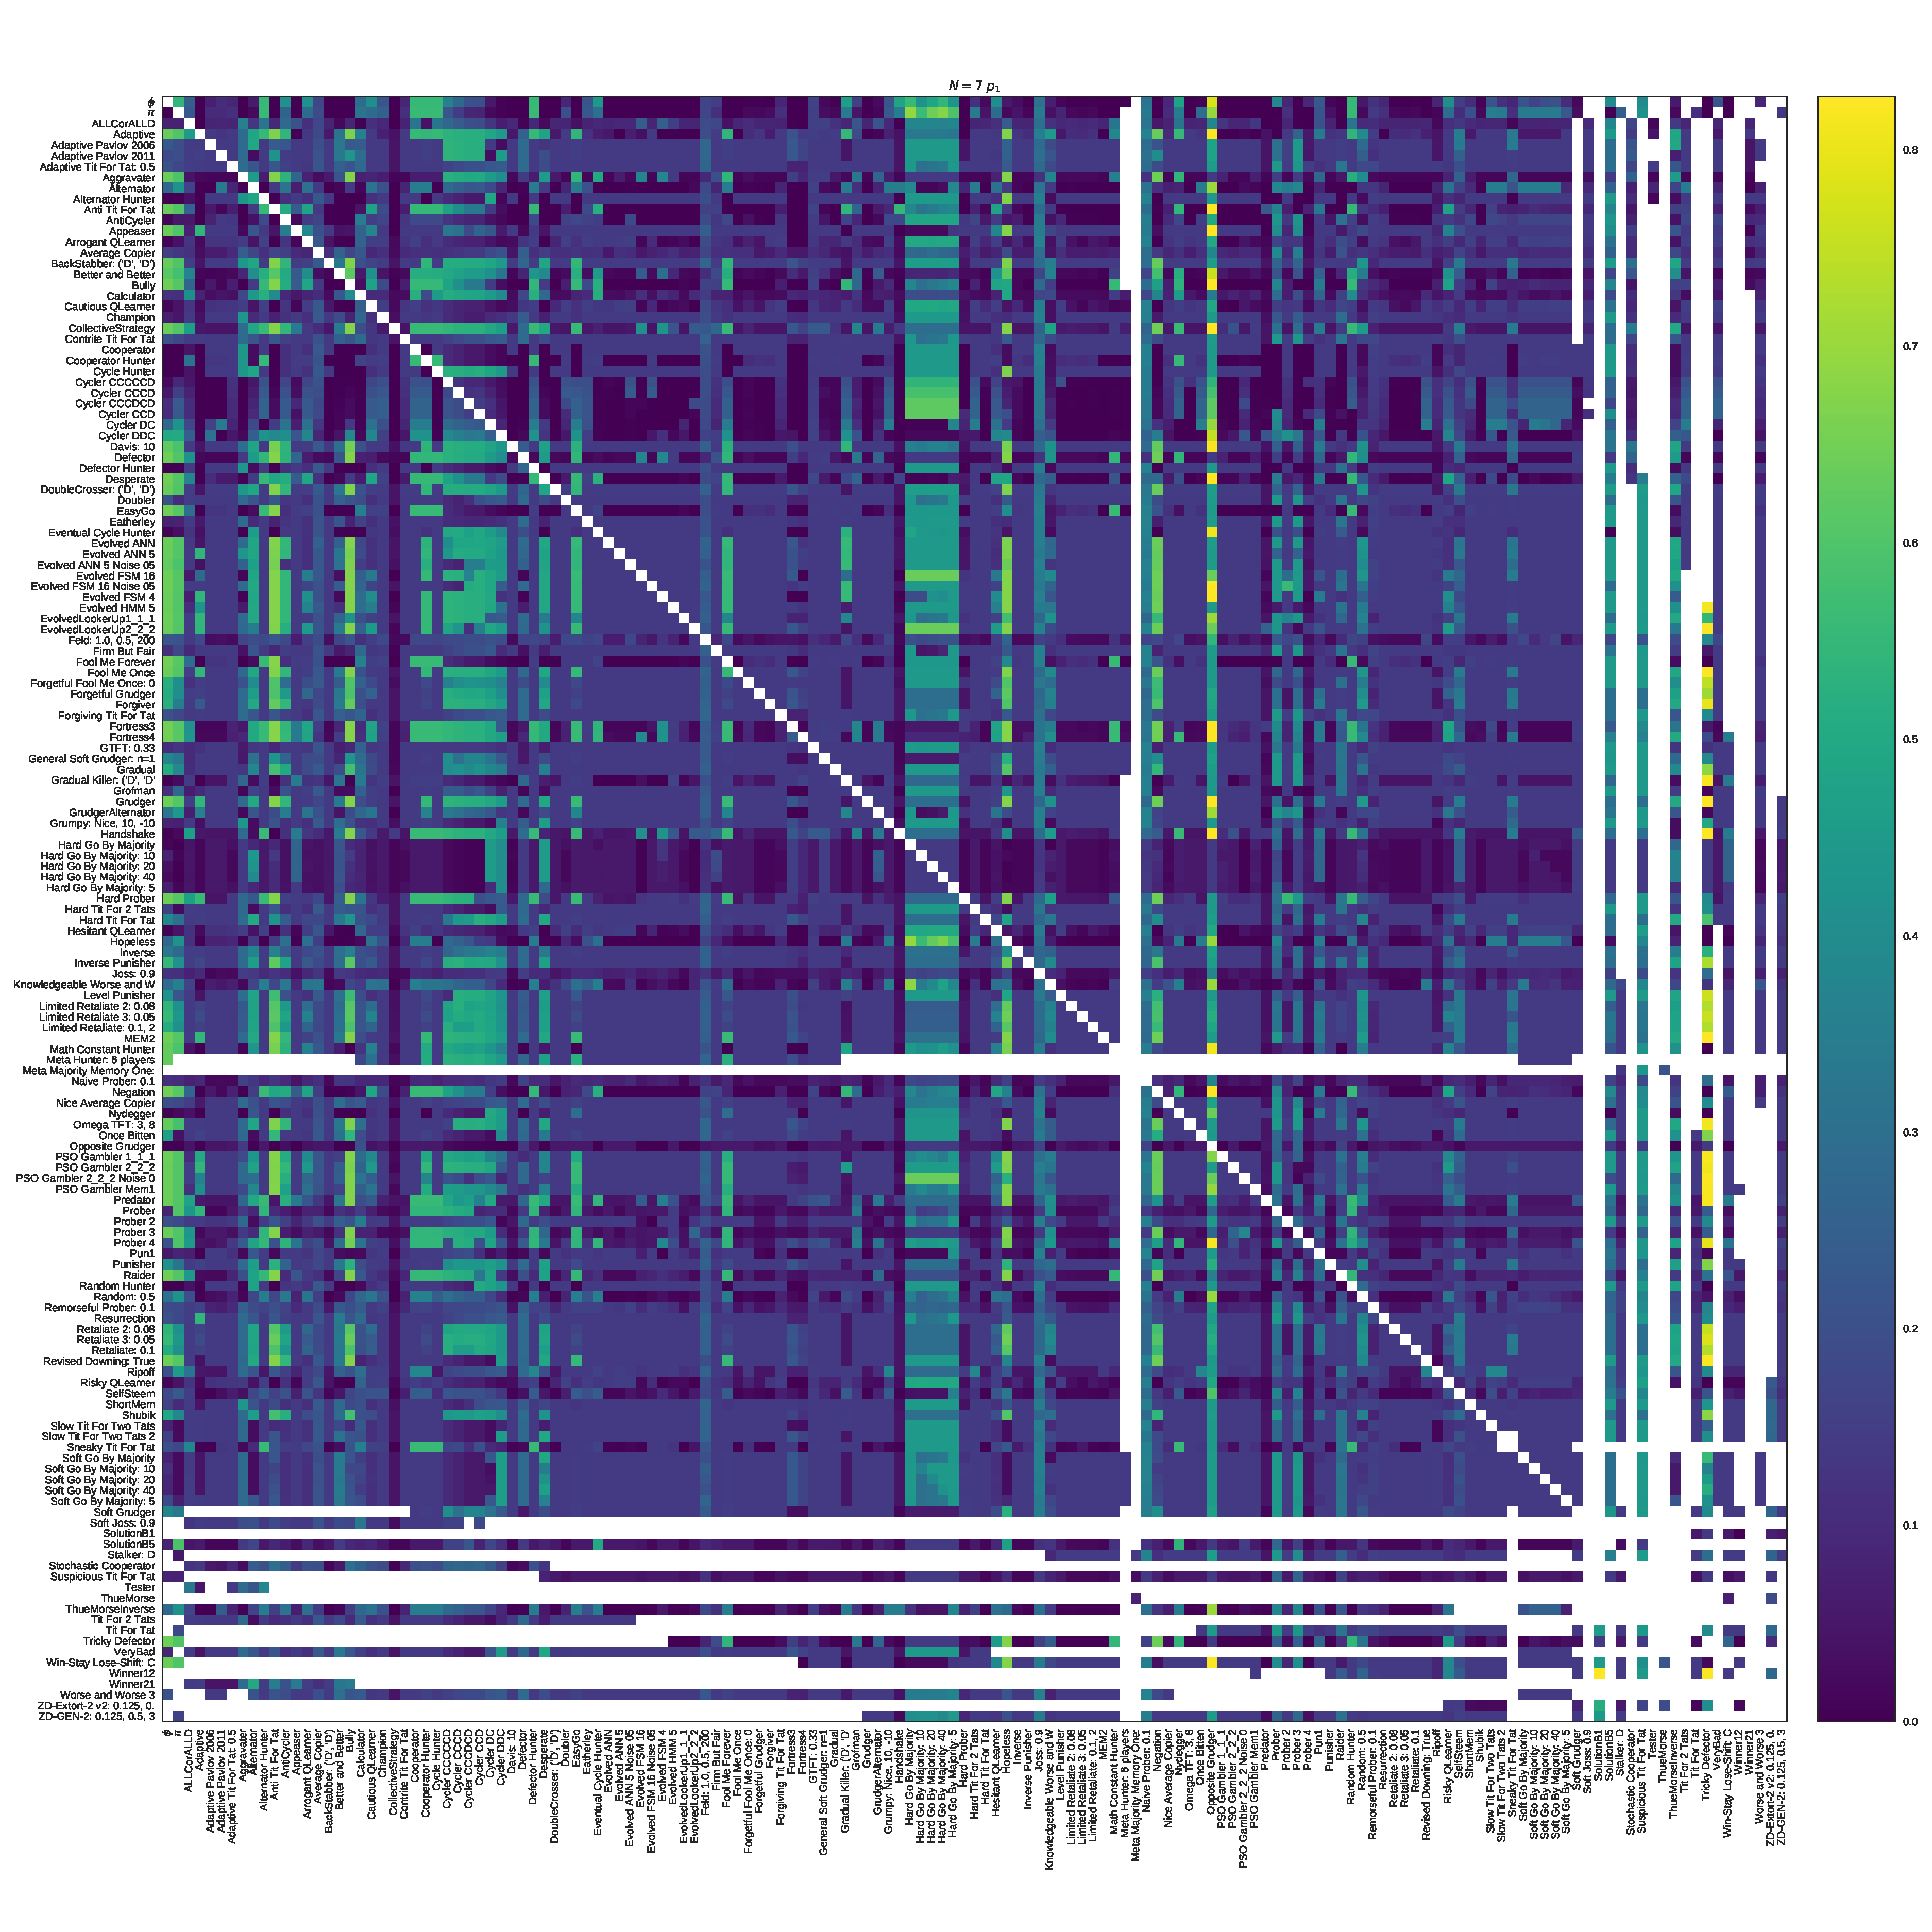
\includegraphics[width=.8\textwidth]{./img/fixation_heatmap_7_invade.pdf}
        \caption{\(N=7\)}
    \end{subfigure}%
    ~
    \begin{subfigure}[t]{.3\textwidth}
        \centering
        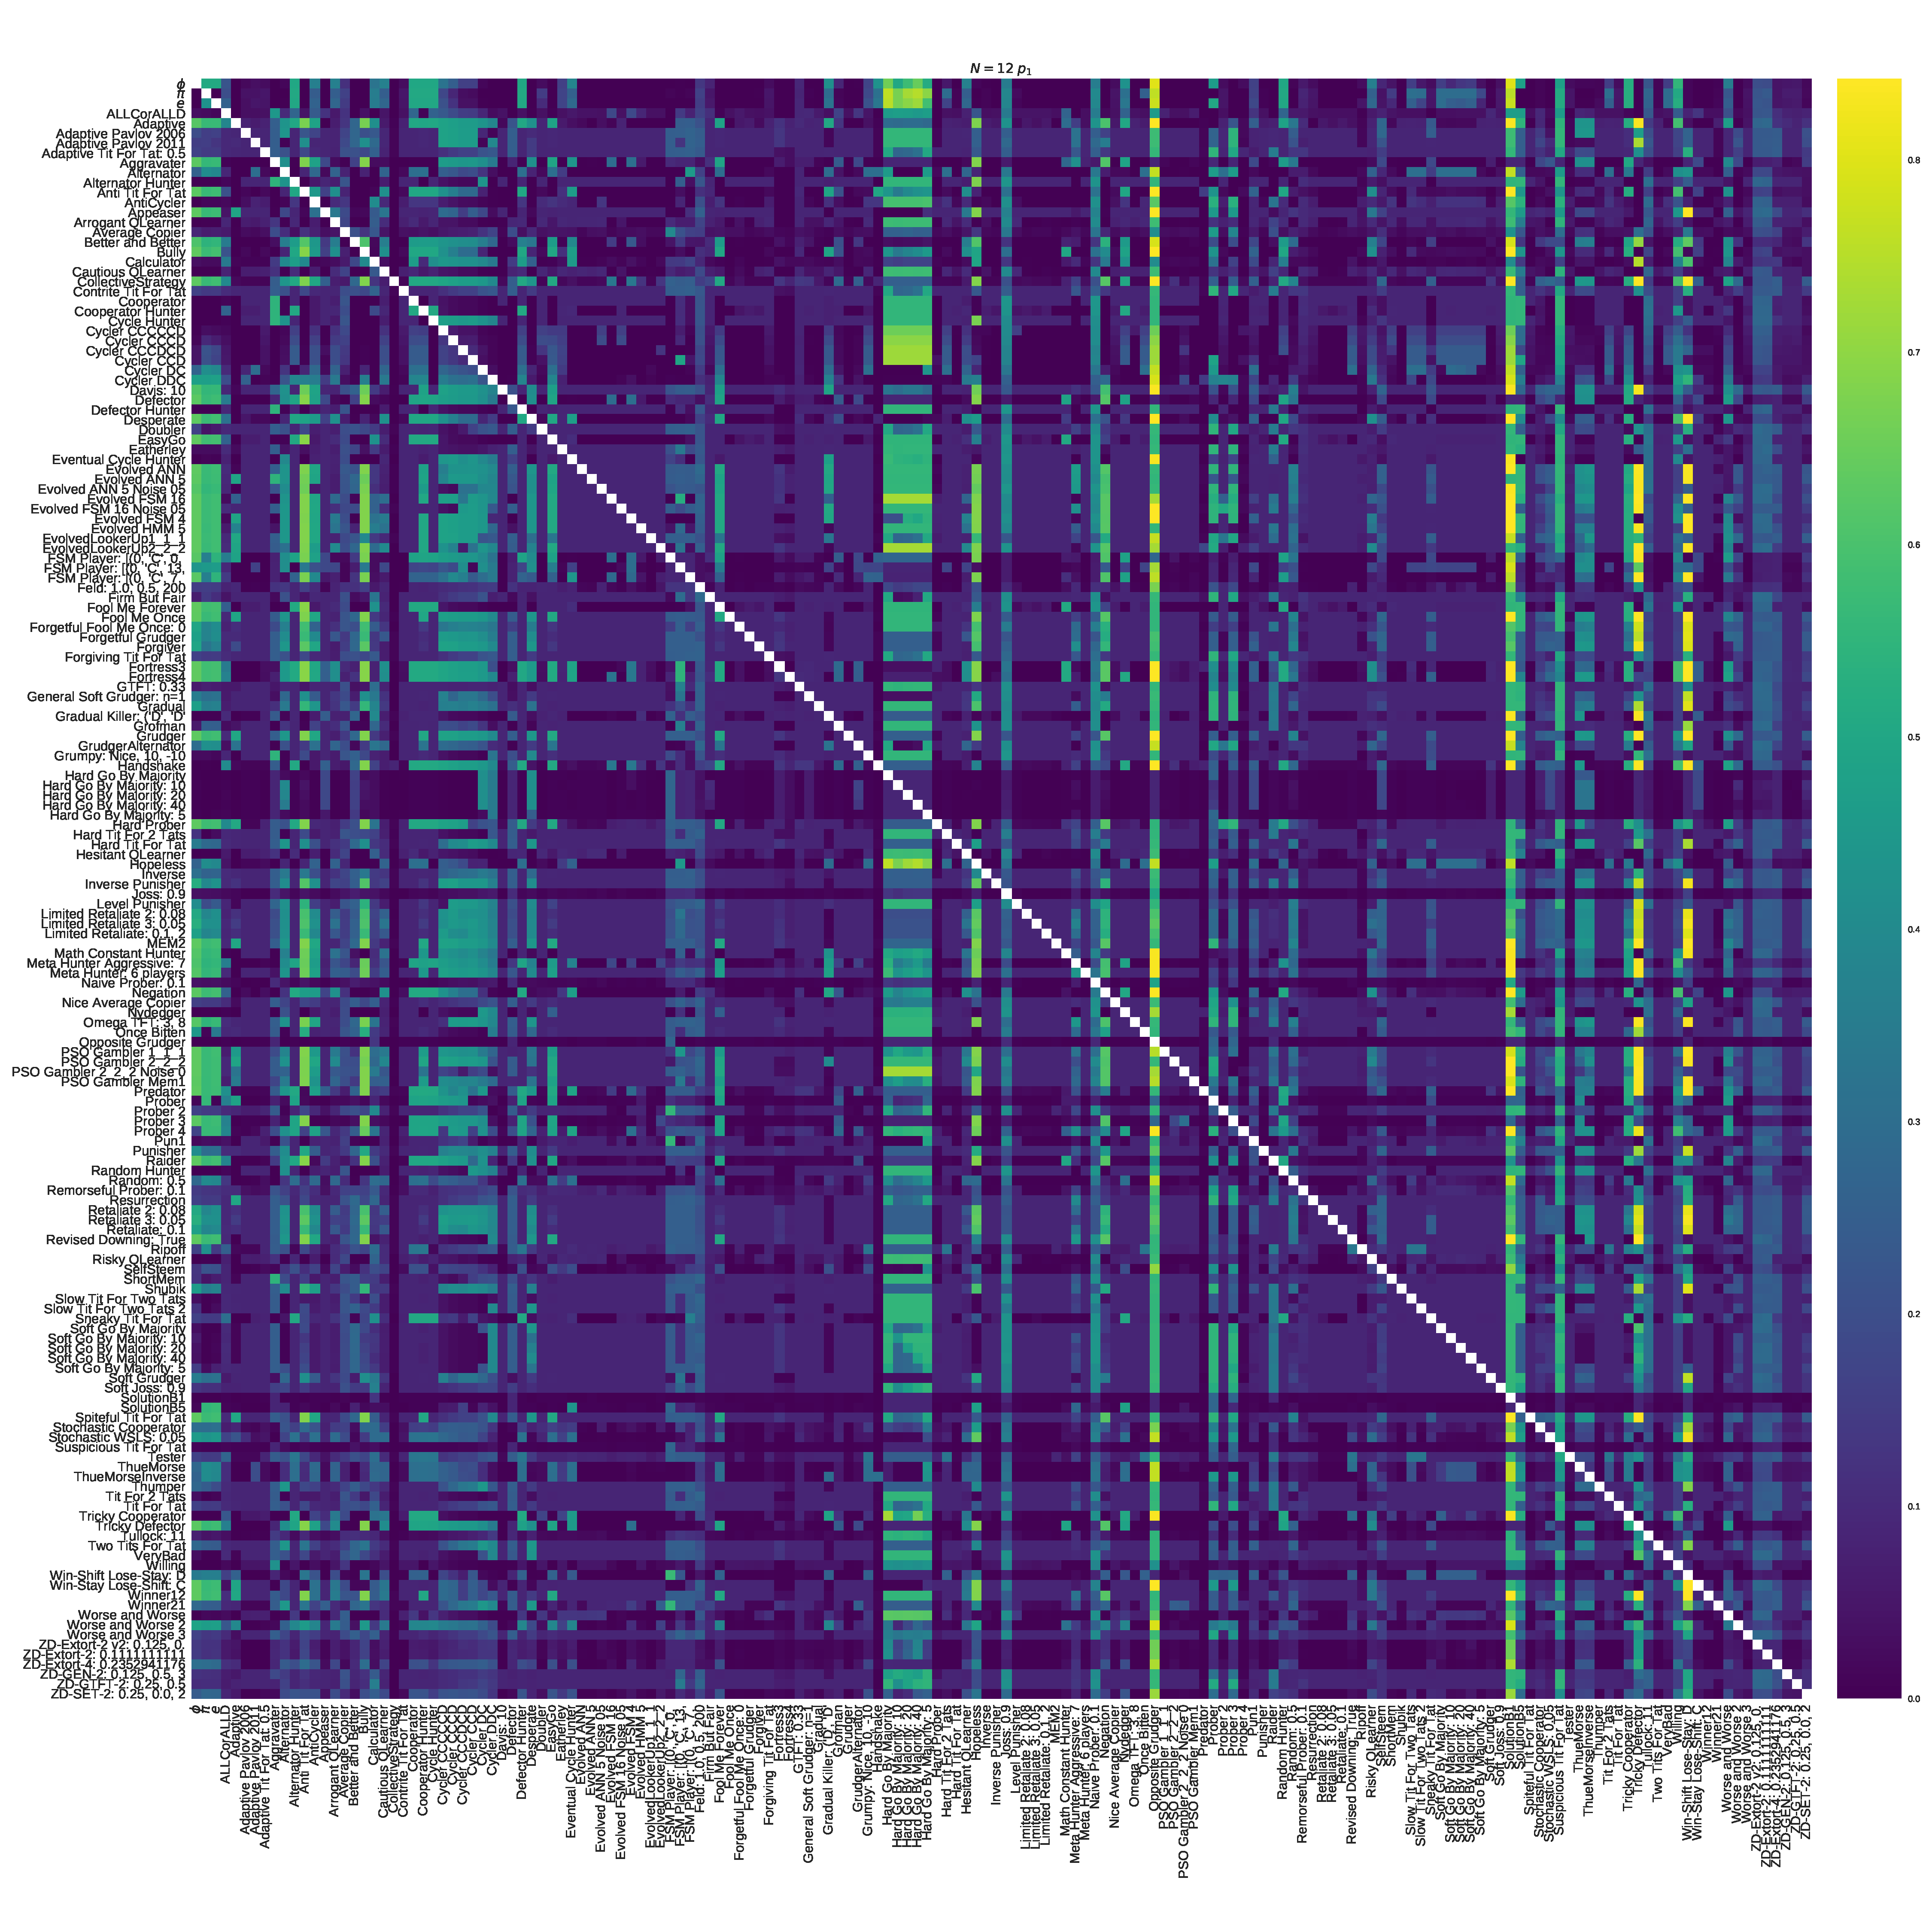
\includegraphics[width=.8\textwidth]{./img/fixation_heatmap_12_invade.pdf}
        \caption{\(N=12\)}

    %TODO Replace N=12 with N=14
    \end{subfigure}%
    %TODO Remove these? I don't feel they are effective

    \caption{Pairwise fixation probability \(x_{1}\) of all strategies}
    \label{fig:fixation_heatmap_invade}
\end{figure}

\begin{figure}[!hbtp]
    \centering
    \begin{subfigure}[t]{.3\textwidth}
        \centering
        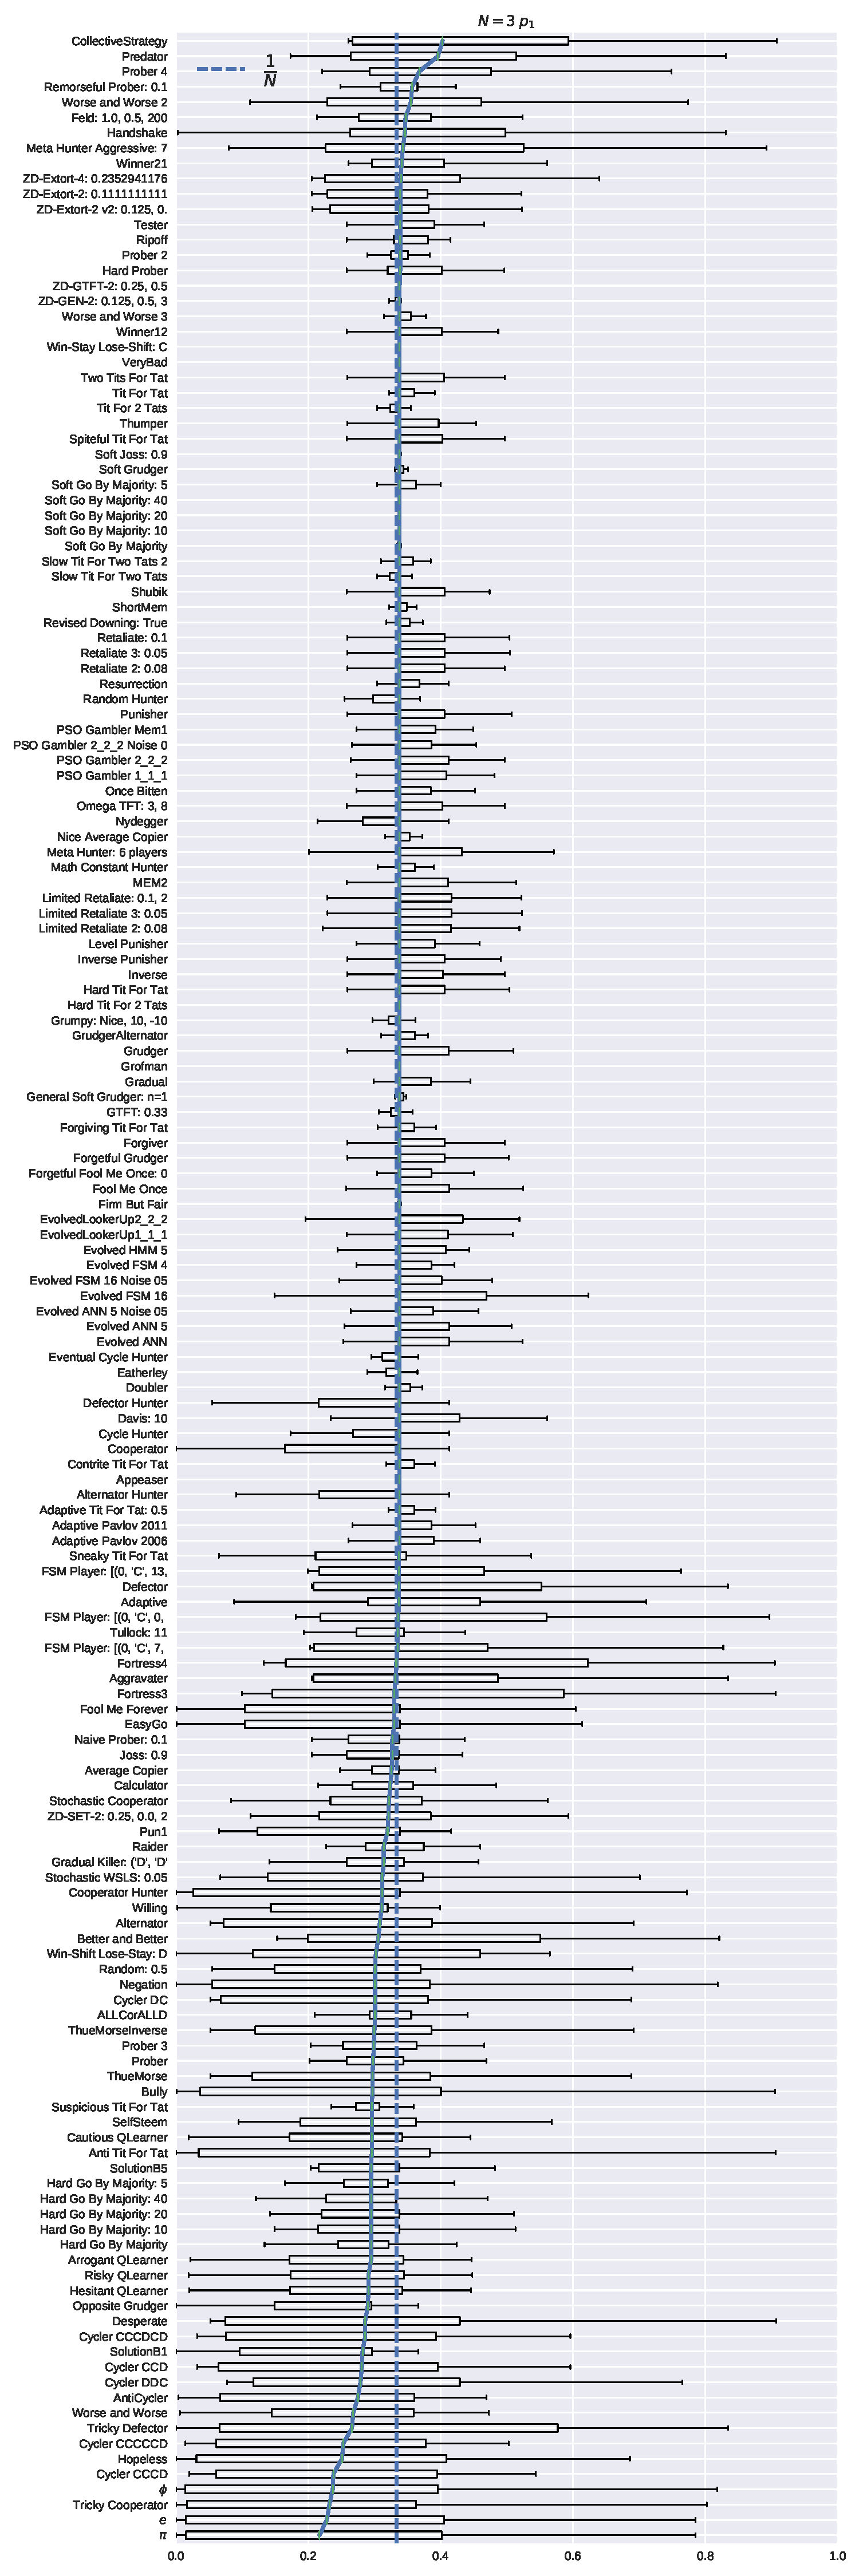
\includegraphics[width=\textwidth]{./img/boxplot_3_invade.pdf}
        \caption{\(N=3\)}
    \end{subfigure}%
    ~
    \begin{subfigure}[t]{.3\textwidth}
        \centering
        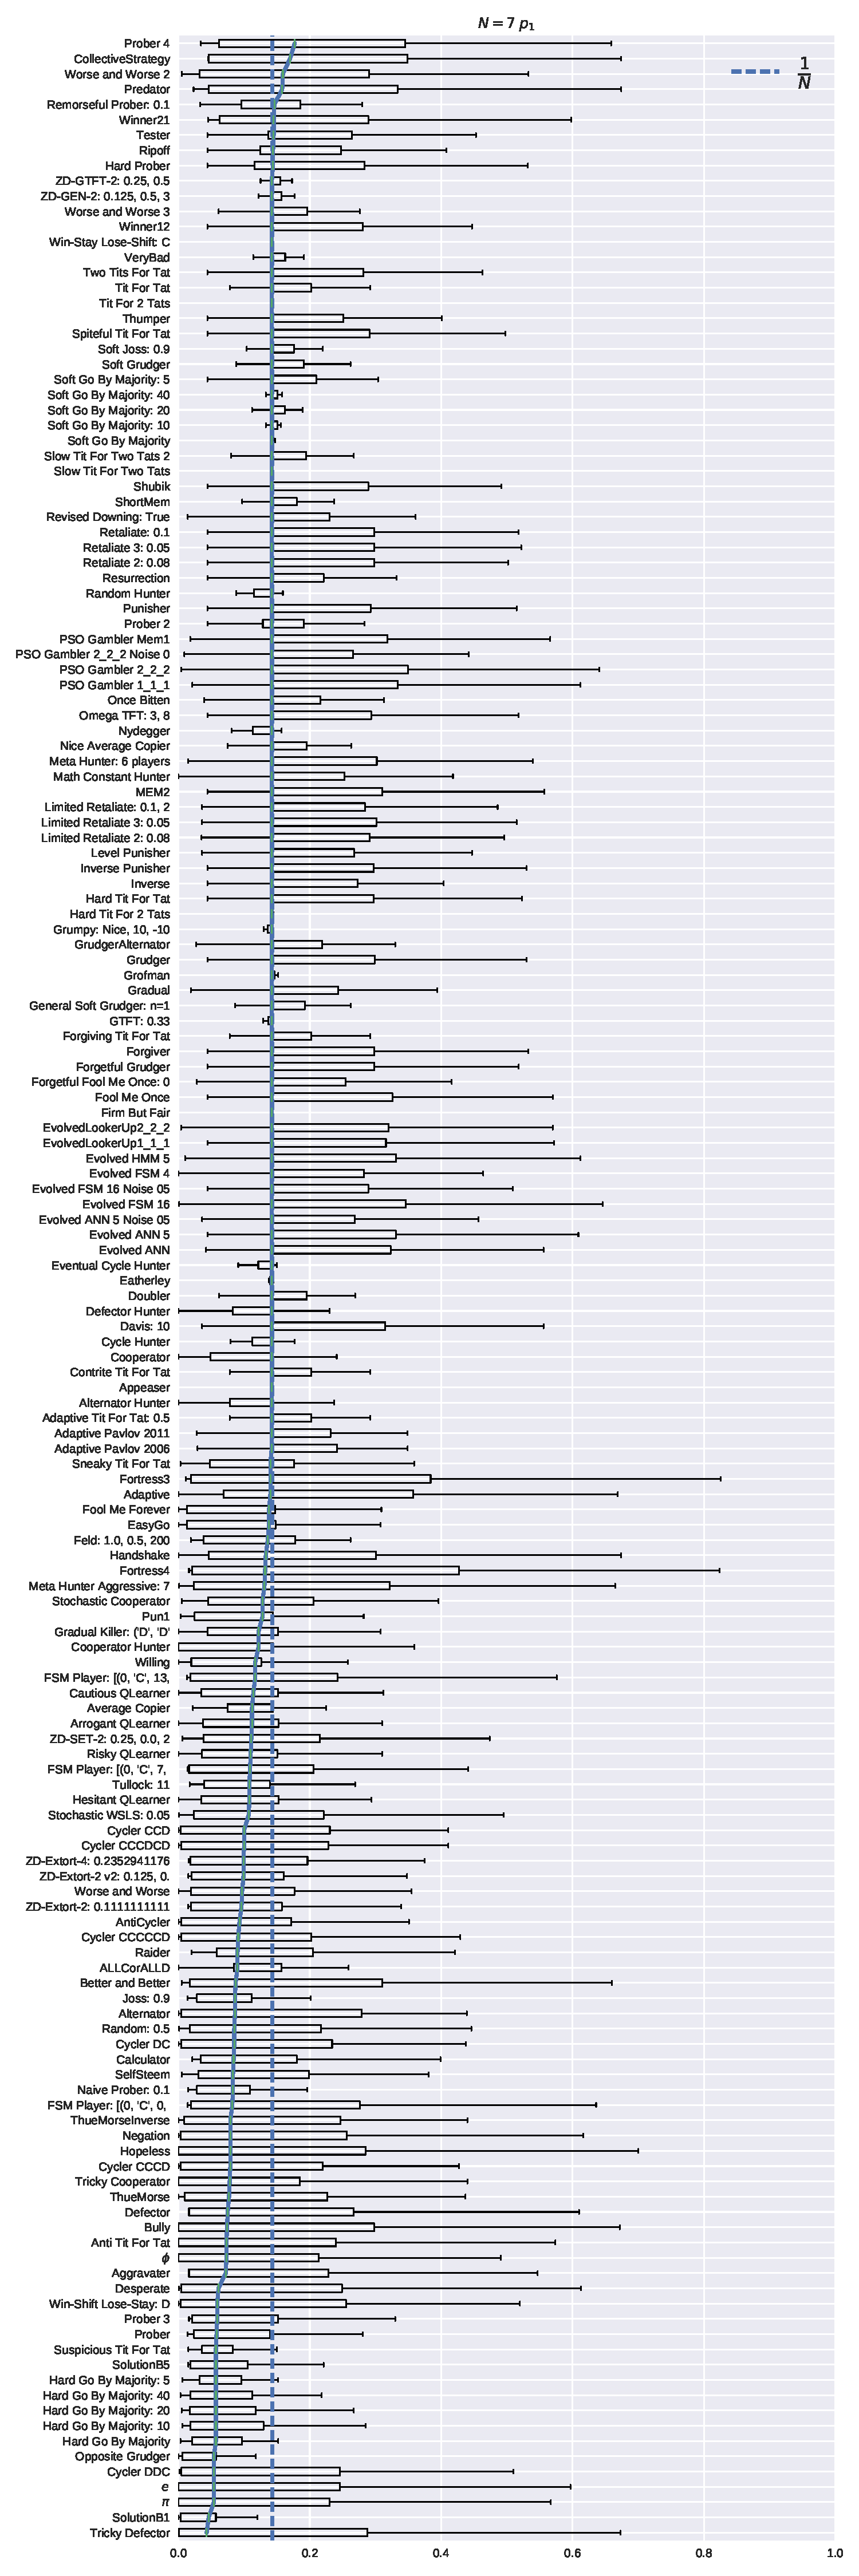
\includegraphics[width=\textwidth]{./img/boxplot_7_invade.pdf}
        \caption{\(N=7\)}
    \end{subfigure}%
    ~
    \begin{subfigure}[t]{.3\textwidth}
        \centering
        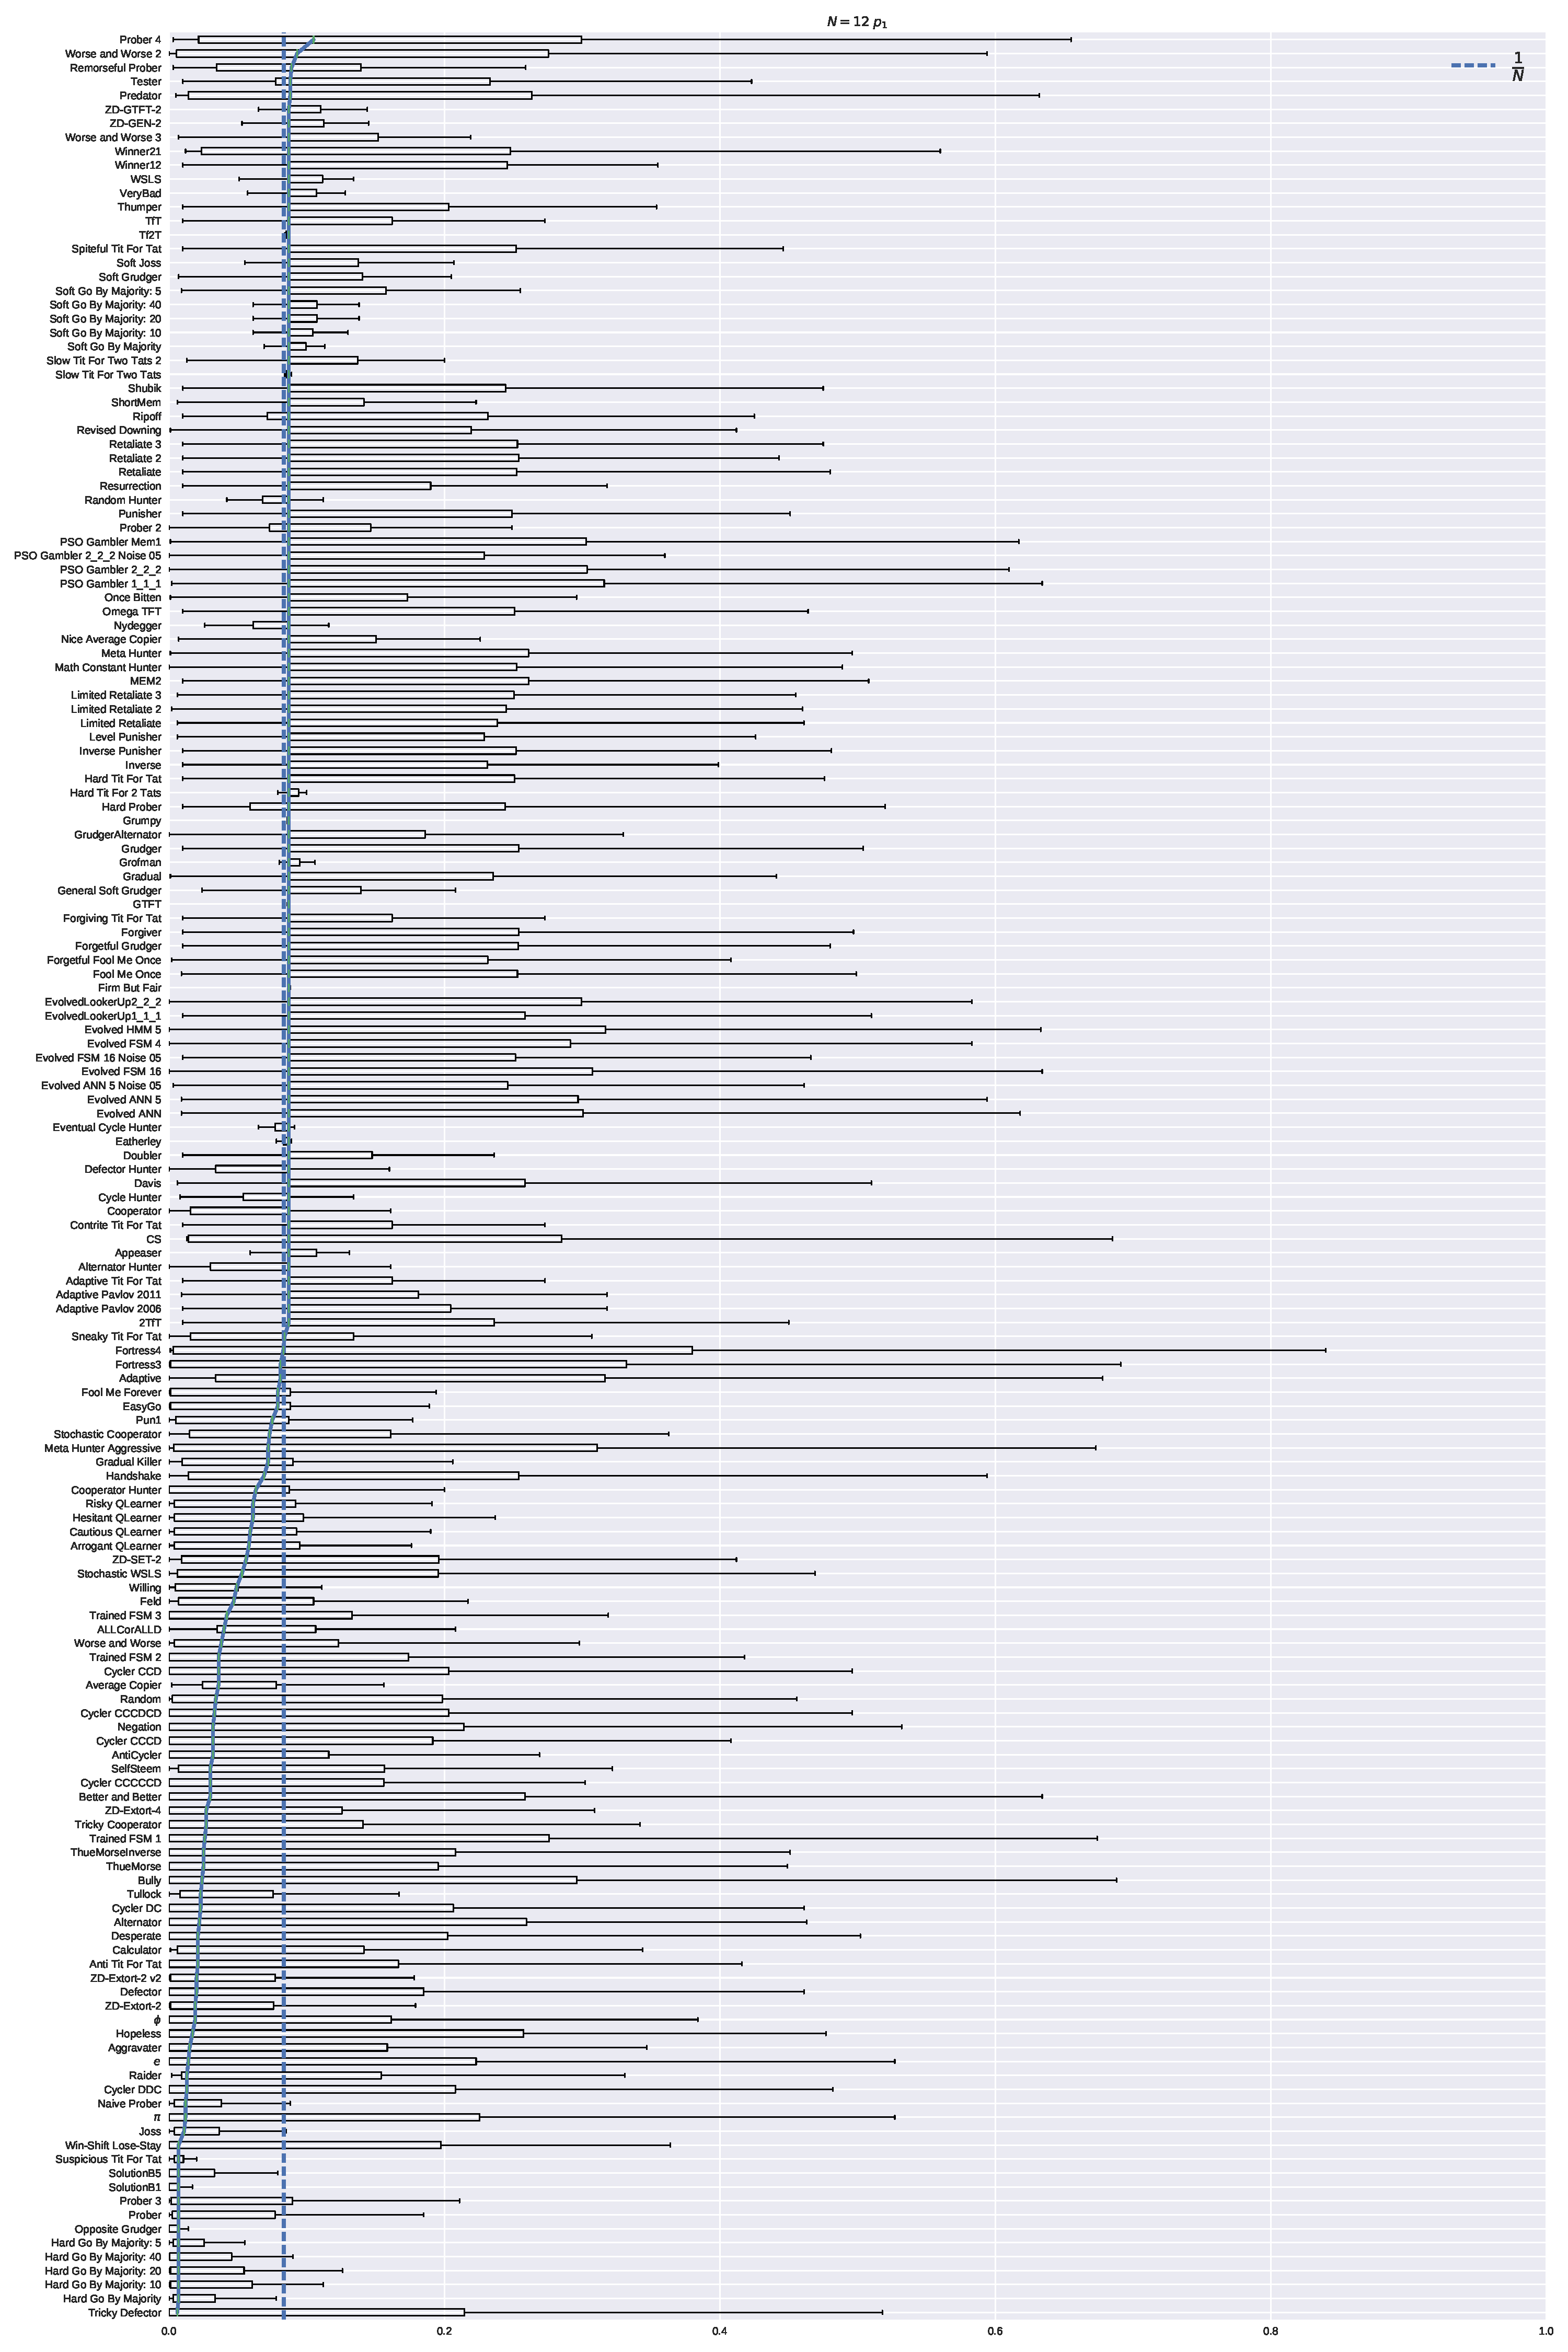
\includegraphics[width=\textwidth]{./img/boxplot_12_invade.pdf}
        \caption{\(N=12\)}
    \end{subfigure}%

    % TODO Replace N=12 with N=14 (when we have more data).
    \caption{Median probabilities \(x_{1}\) of all strategies as well as the
    neutral fixation probability}
    \label{fig:fixation_boxplot_invade}
\end{figure}

For \(N\in\{3, 7, 12\}\) the top five strategies are given in
% TODO Change N=12 to N=14
Tables~\ref{tbl:top_five_invade}.

\begin{table}[!hbtp]
    \begin{subfigure}[t]{\textwidth}
        \centering
        \begin{tabular}{lrrl}
\toprule
   Player &  Mean $p_1$ &  Memory Depth & Stochastic \\
\midrule
       CS &    0.447761 &            \(\infty\) &      False \\
  Grudger &    0.431264 &            \(\infty\) &      False \\
     MEM2 &    0.427804 &            \(\infty\) &      False \\
      TF3 &    0.426736 &            16 &      False \\
 Prober 4 &    0.424215 &            \(\infty\) &      False \\
\bottomrule
\end{tabular}

        \caption{\(N=3\)}
    \end{subfigure}
    \begin{subfigure}[t]{\textwidth}
        \centering
        \begin{tabular}{llr}
\toprule
{} &                   Player &  Mean $p_1$ \\
\midrule
1  &           Evolved FSM 16 &      0.2523 \\
2  &        PSO Gambler 2\_2\_2 &      0.2467 \\
3  &             Fool Me Once &      0.2459 \\
4  &            Evolved ANN 5 &      0.2450 \\
5  &              Evolved ANN &      0.2449 \\
6  &     EvolvedLookerUp2\_2\_2 &      0.2443 \\
7  &                  Grudger &      0.2442 \\
8  &                     MEM2 &      0.2436 \\
9  &                      \textbf{TF3} &      0.2430 \\
10 &        PSO Gambler 1\_1\_1 &      0.2404 \\
11 &                       CS &      0.2395 \\
12 &  Evolved FSM 16 Noise 05 &      0.2394 \\
13 &            Evolved HMM 5 &      0.2390 \\
14 &              Meta Hunter &      0.2385 \\
15 &                    Davis &      0.2379 \\
16 &         PSO Gambler Mem1 &      0.2348 \\
\bottomrule
\end{tabular}

        \caption{\(N=7\)}
    \end{subfigure}
    \begin{subfigure}[t]{\textwidth}
        \centering
        \begin{tabular}{lrrl}
\toprule
               Player &  Mean $p_1$ &  Memory Depth & Stochastic \\
\midrule
       Evolved FSM 16 &    0.217374 &            16 &      False \\
    PSO Gambler 2\_2\_2 &    0.210914 &            \(\infty\) &       True \\
 EvolvedLookerUp2\_2\_2 &    0.208779 &            \(\infty\) &      False \\
          Evolved ANN &    0.208313 &            \(\infty\) &      False \\
        Evolved ANN 5 &    0.206644 &            \(\infty\) &      False \\
\bottomrule
\end{tabular}

        \caption{\(N=12\)}
    \end{subfigure}
    %TODO Change N=12 to N=14
    \caption{Properties of top five invaders}
    \label{tbl:top_five_invade}
\end{table}

It can be seen that apart from the Collective strategy, none of the strategies
of Table~\ref{tbl:summary_top_2} perform well for \(N\in\{3, 7, 12\}\). The new
% TODO Change N=12 to N=14
high performing strategies are:

\begin{itemize}
    \item Predator, a finite state machine described in~\cite{Ashlock2006}.
    \item Prober 4, complex strategy with an initial 20 move sequence of
        cooperations and defections~\cite{prison}. This initial sequence serves
        as some kind of handshake.
    \item Remorseful Prober, a strategy that will not immediately retaliate when
        it recognises that the opponent is itself retaliating to a random
        defection~\cite{Li2011}.
    \item  Worse and worse 2: plays tit for tat for 20 moves and then defects
        with with growing probability~\cite{prison}.
    \item Tester: a strategy submitted to the second of Axelrod's tournaments
        \cite{Axelrod1980b}.
        % TODO Check if this list is still correct for N=14
\end{itemize}

As well as noting that the memory length and complexity of these strategies are
quite complex it is interesting to note that none of them are akin to memory one
strategies. Most are not stochastic.

In the next section the performance in terms of \(x_{N-1}\) will be described:
what strategies are particularly good at resisting an invasion.

\subsection{Strong resistors}\label{sec:strong_resistors}

Figures~\ref{fig:fixation_heatmap_resist} show \(x_{N-1}\)
the players along the vertical axis when matched against the players on the
horizontal axis. It can be seen that as the population size \(N\) increases the
probability of resistance increases.
This information is summarised in Figure~\ref{fig:fixation_boxplot_resist}
showing the median fixation as well as the neutral fixation for each given
scenario.

\begin{figure}[!hbtp]
    \centering
    \begin{subfigure}[t]{.3\textwidth}
        \centering
        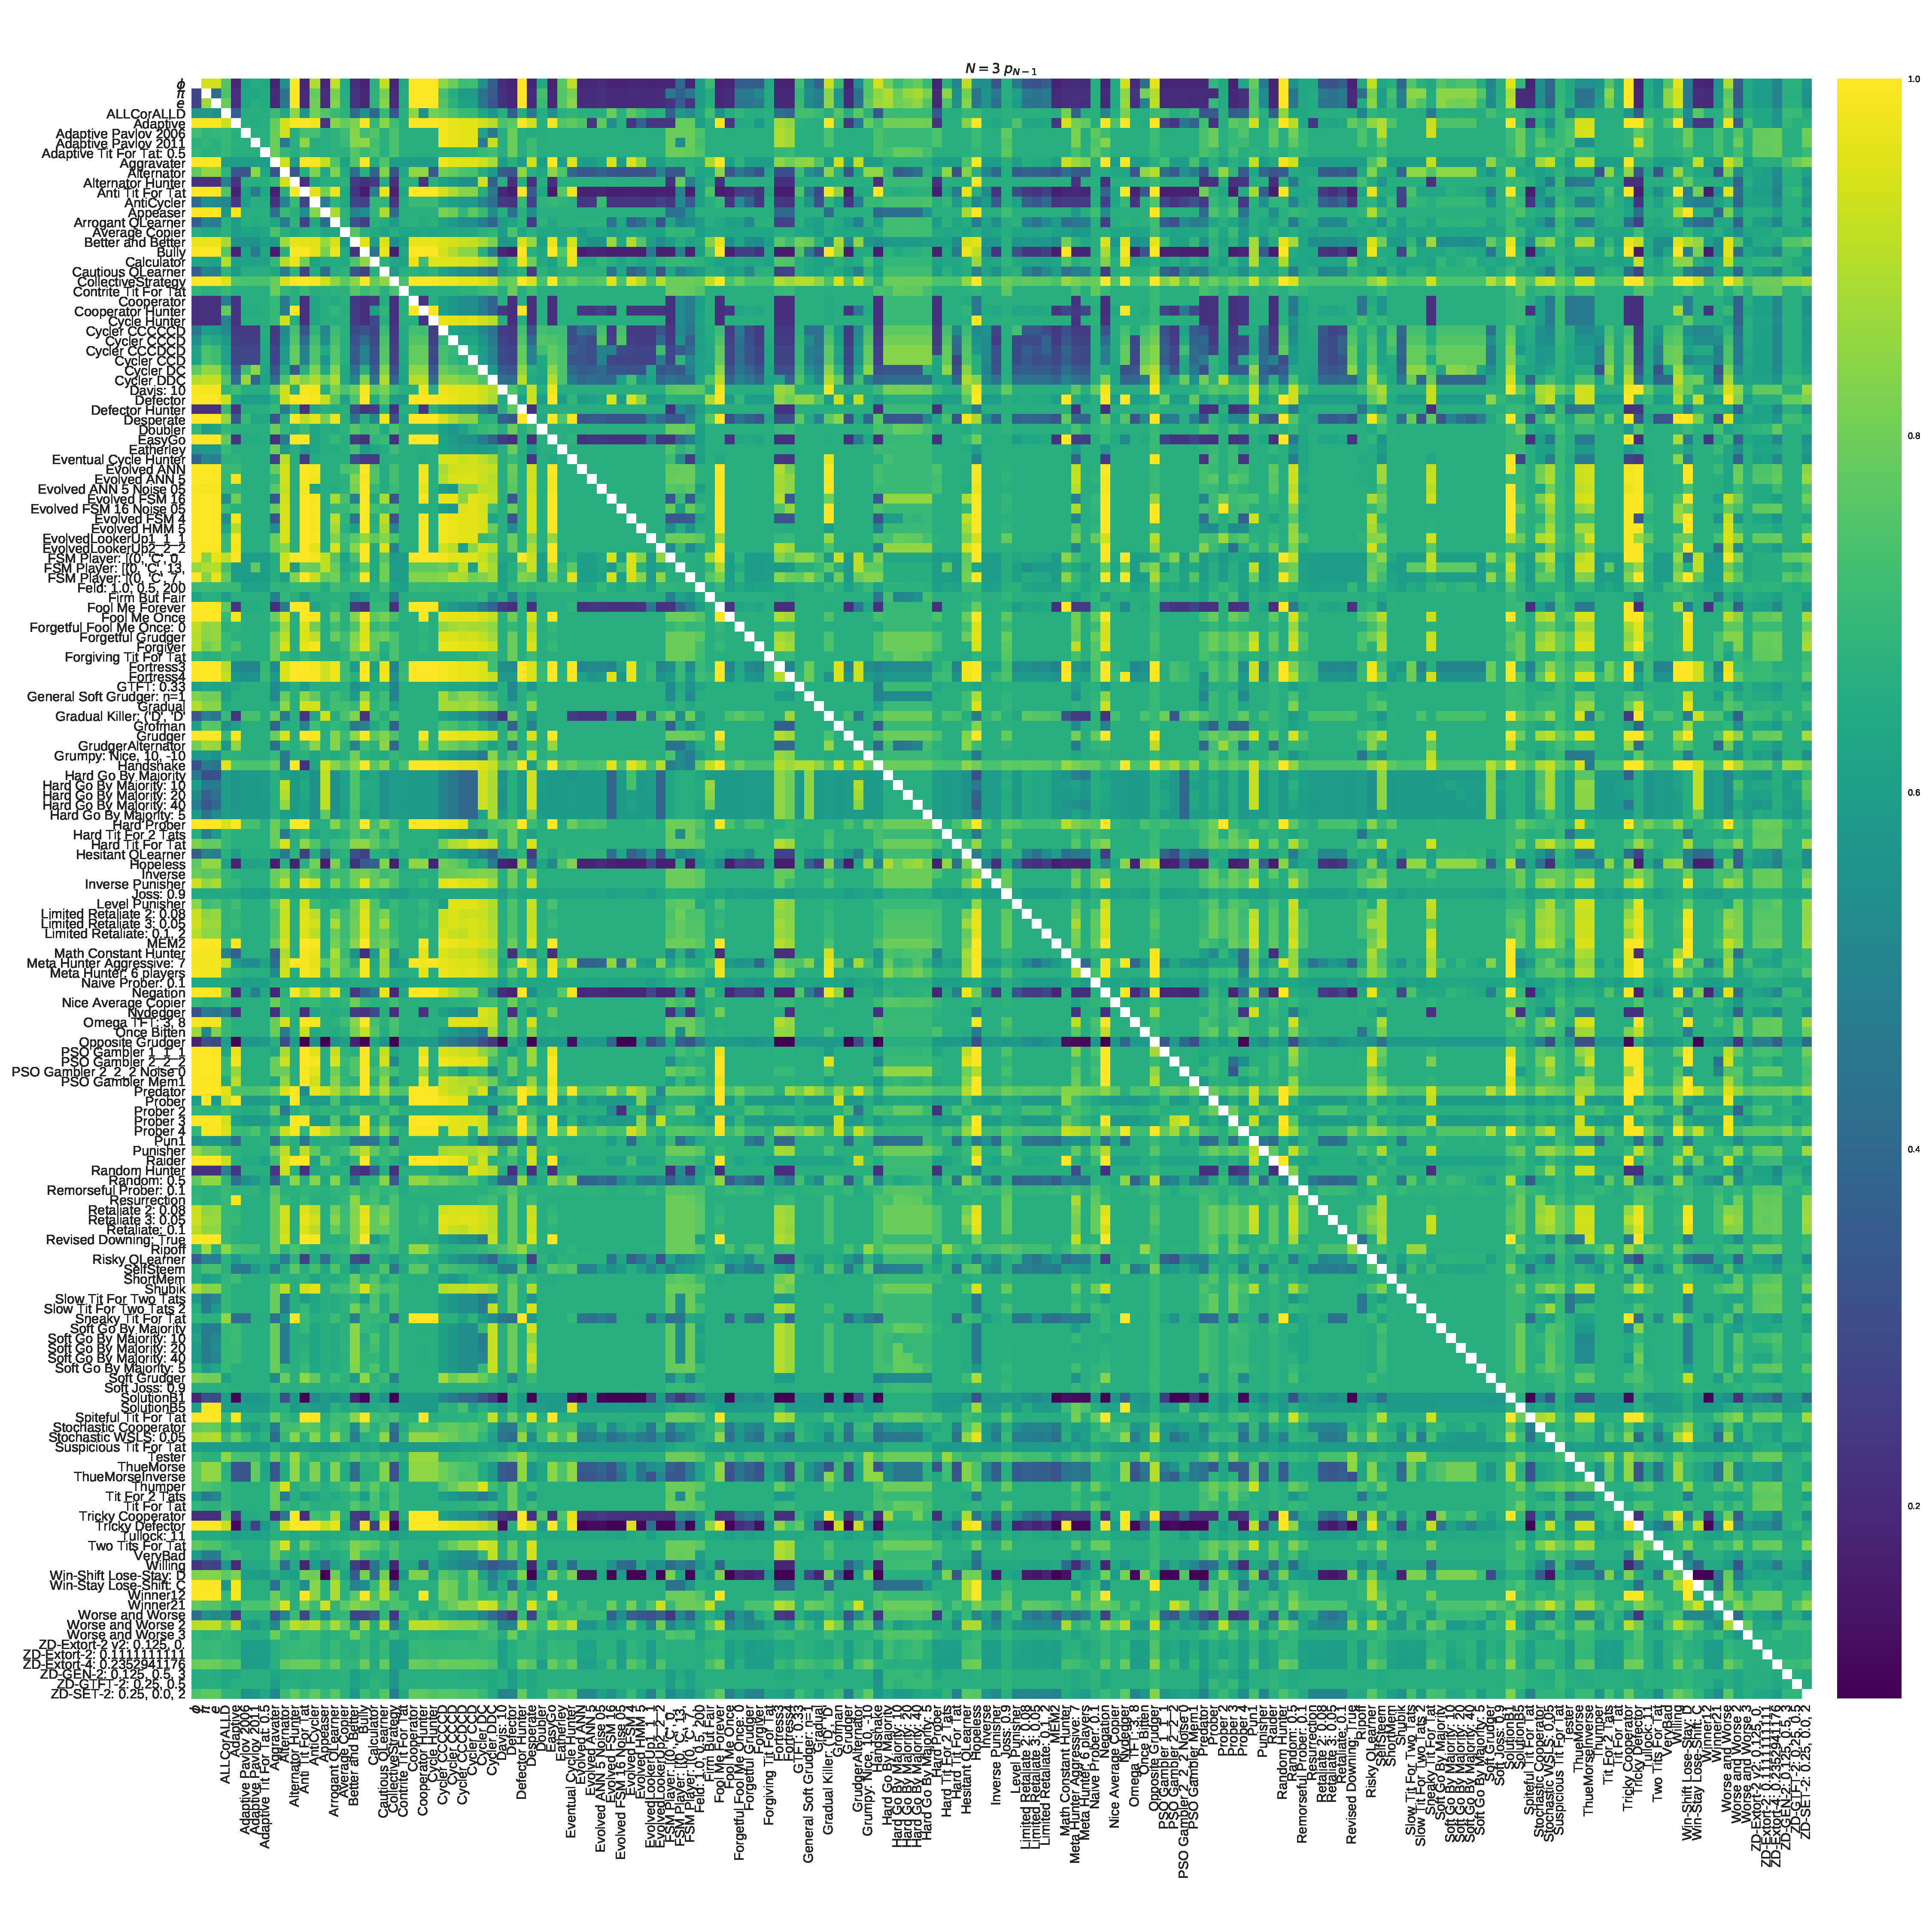
\includegraphics[width=.8\textwidth]{./img/fixation_heatmap_3_resist.pdf}
        \caption{\(N=3\)}
    \end{subfigure}%
    ~
    \begin{subfigure}[t]{.3\textwidth}
        \centering
        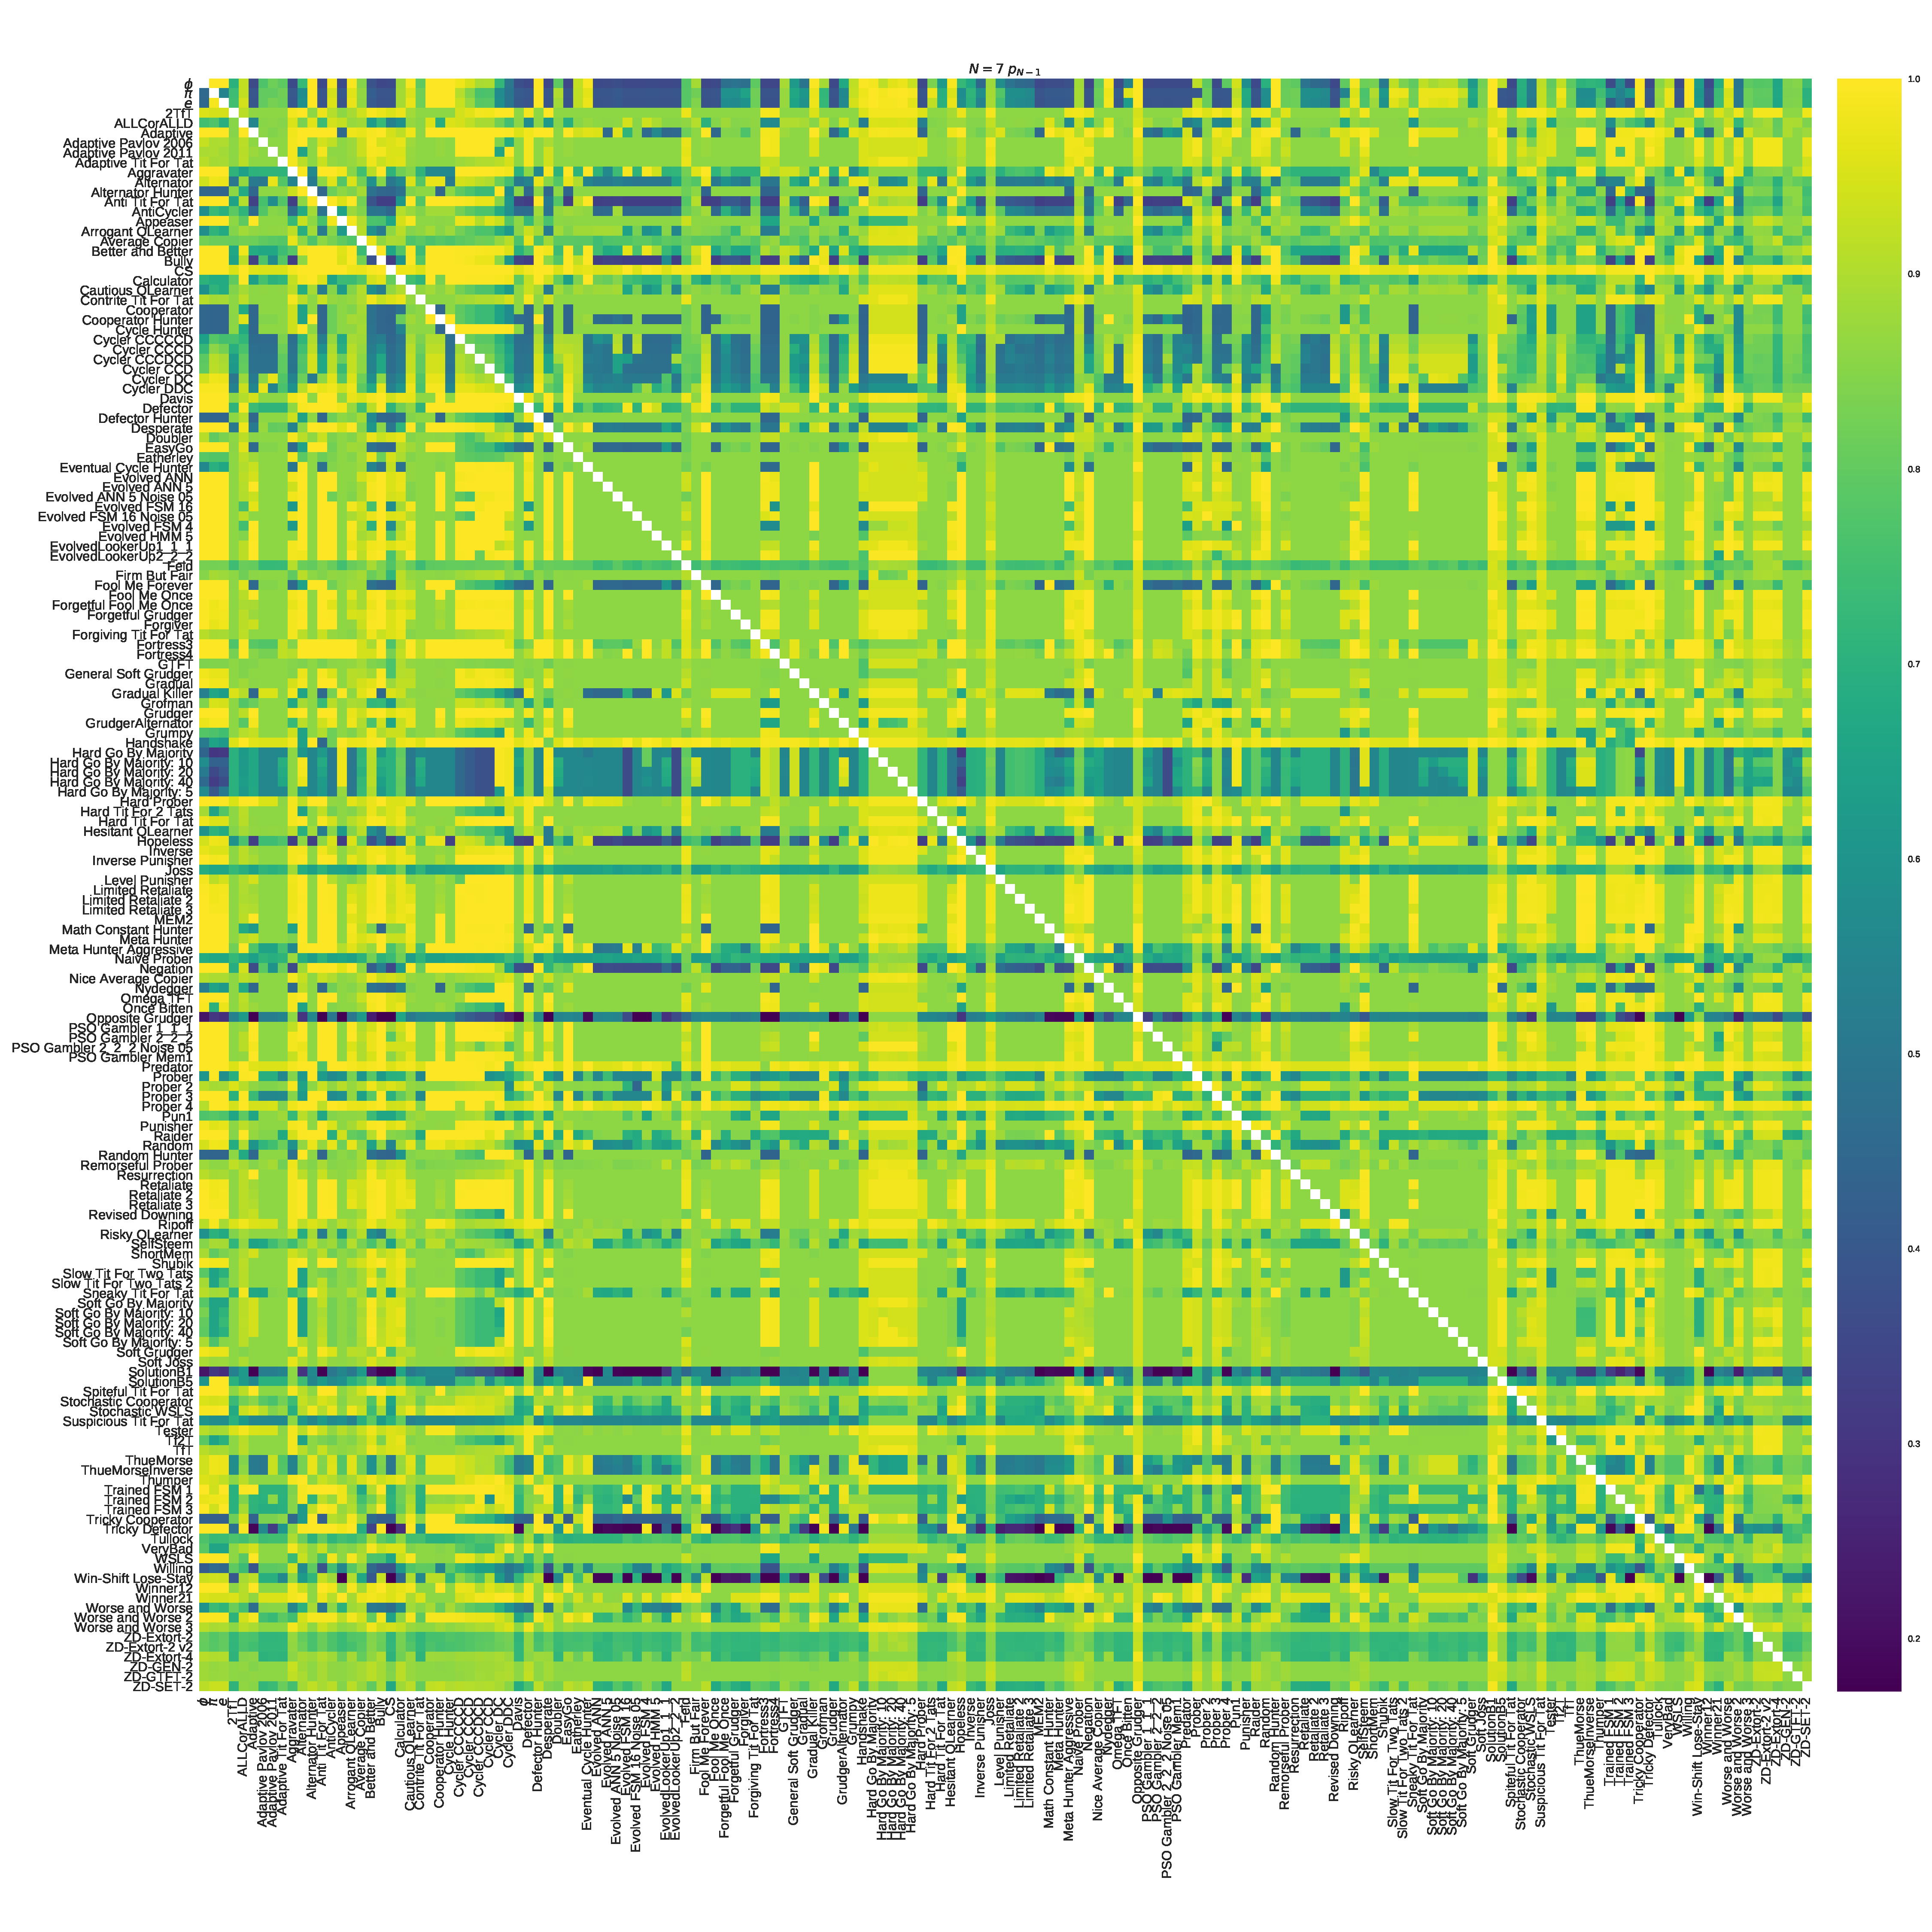
\includegraphics[width=.8\textwidth]{./img/fixation_heatmap_7_resist.pdf}
        \caption{\(N=7\)}
    \end{subfigure}%
    ~
    \begin{subfigure}[t]{.3\textwidth}
        \centering
        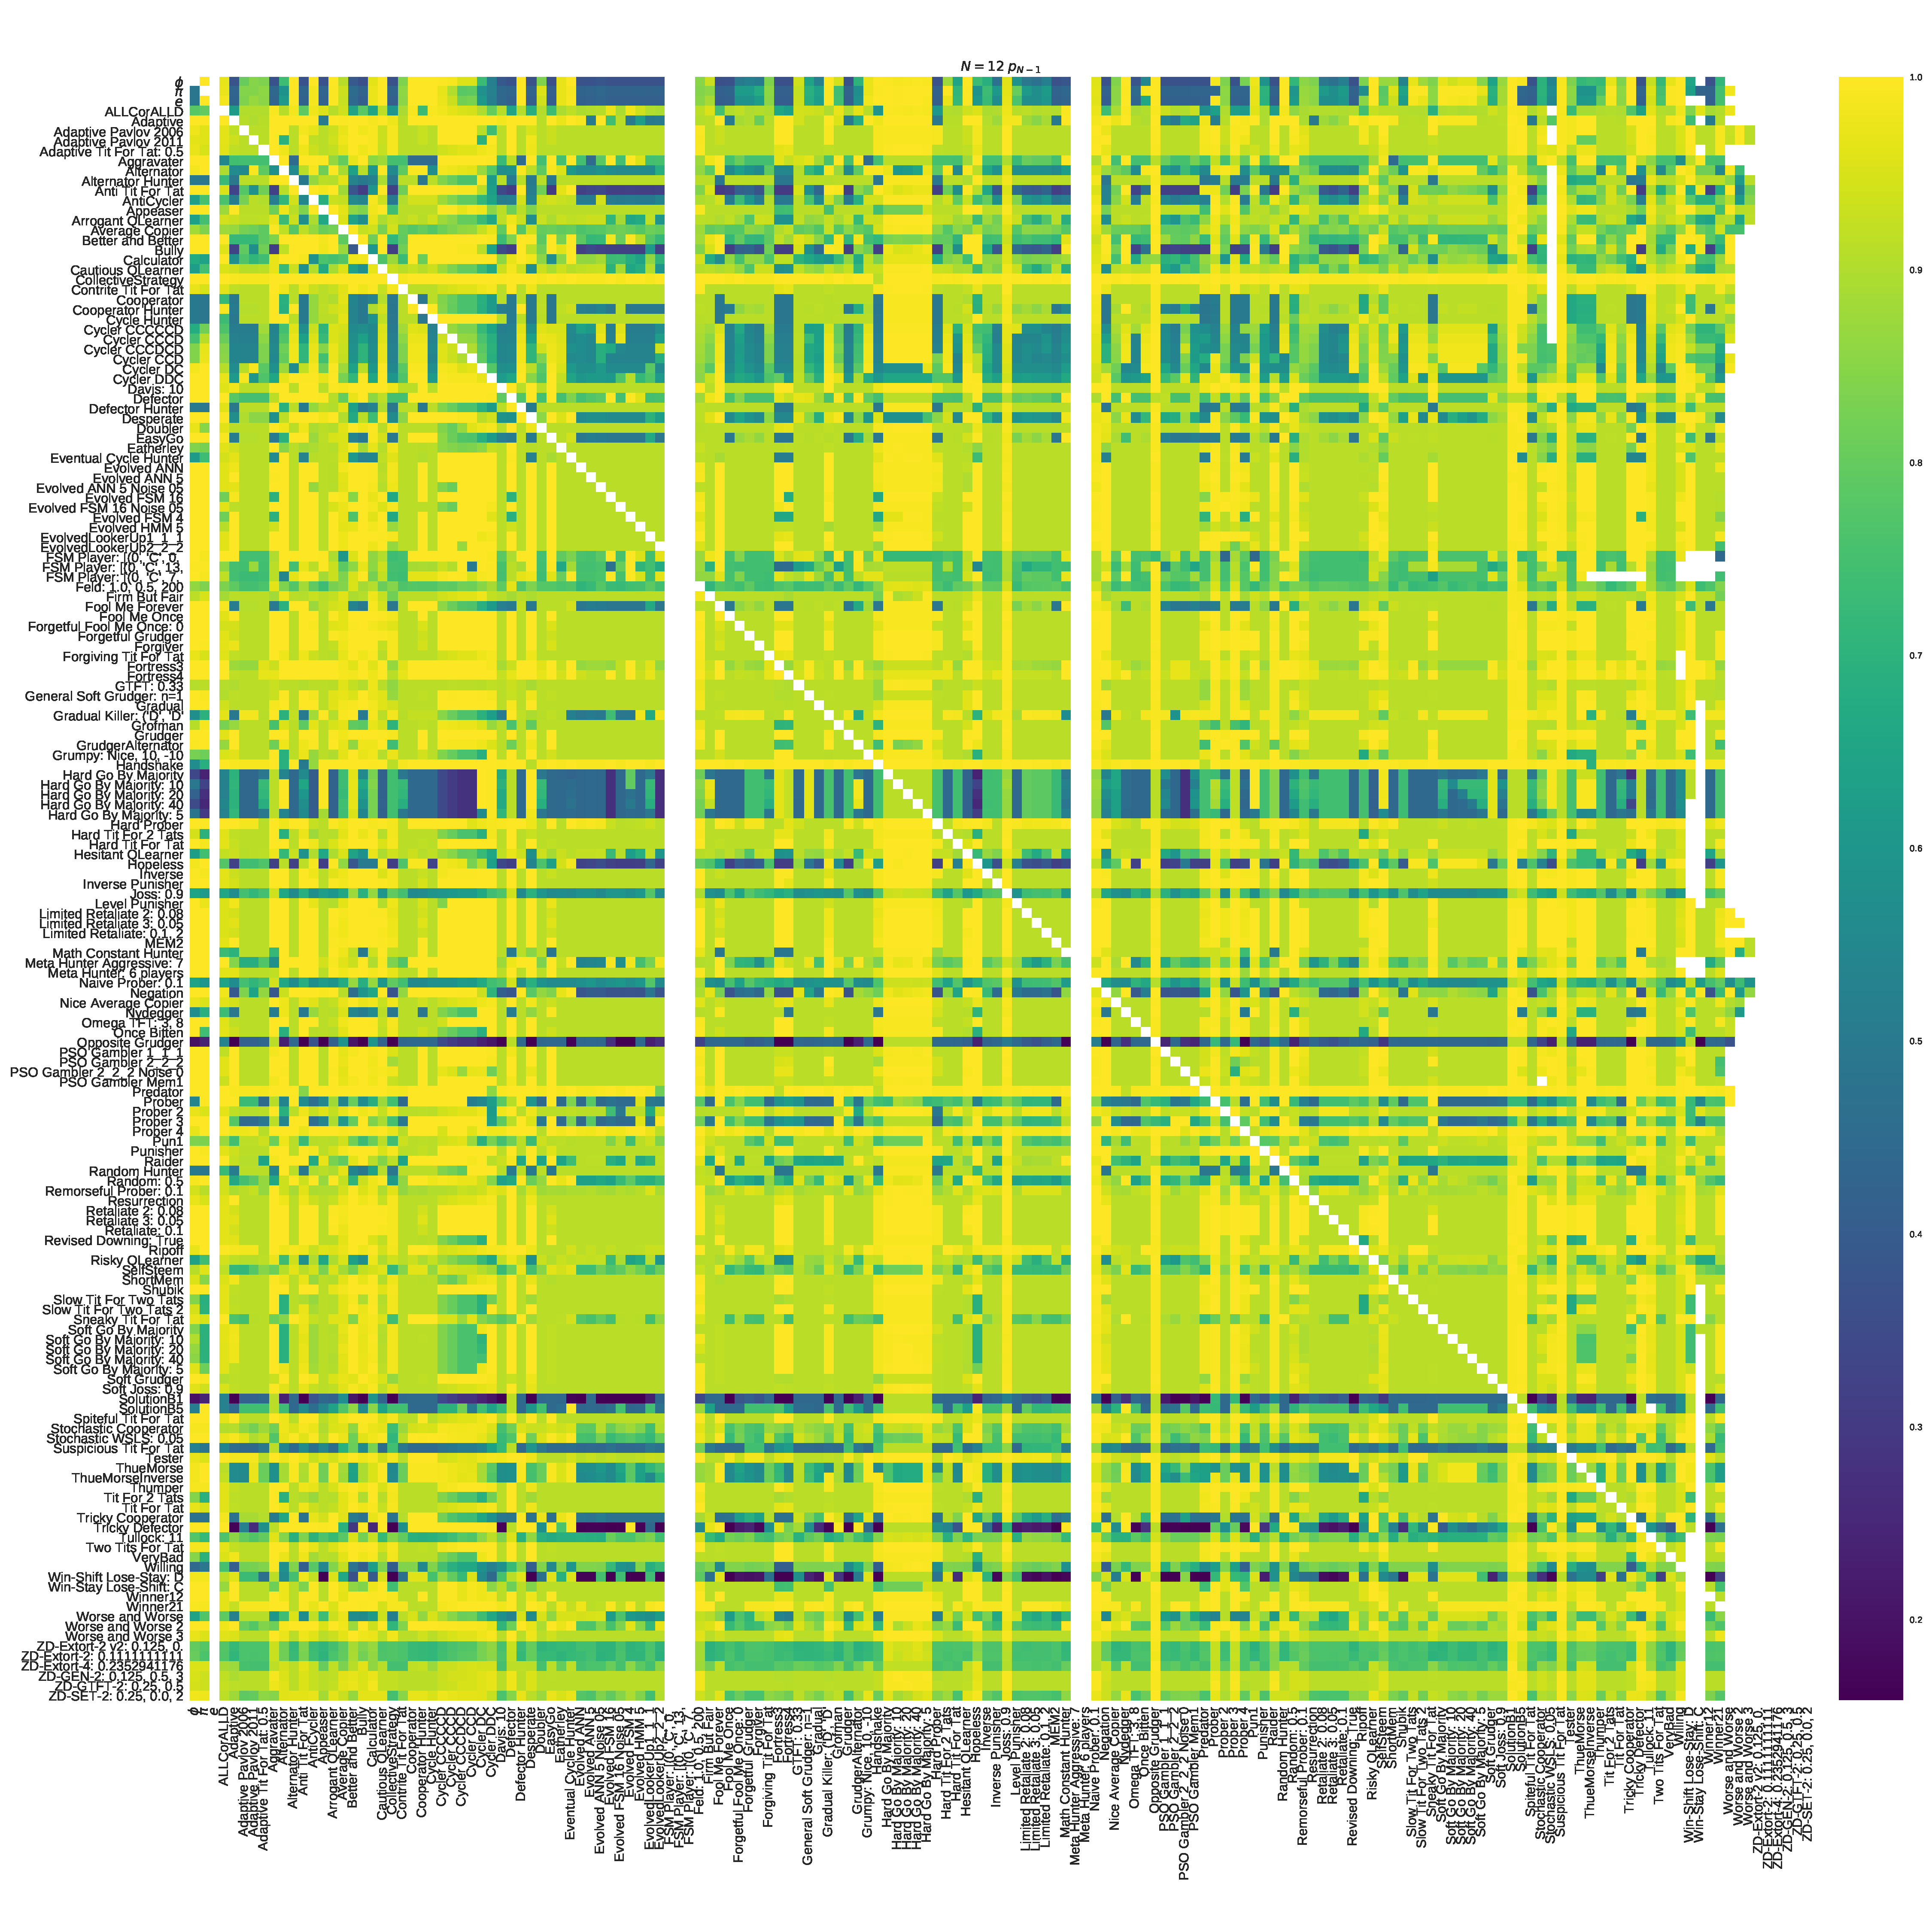
\includegraphics[width=.8\textwidth]{./img/fixation_heatmap_12_resist.pdf}
        \caption{\(N=12\)}

    %TODO Replace N=12 with N=14
    \end{subfigure}%
    %TODO Remove these? I don't feel they are effective

    \caption{Pairwise fixation probability \(x_{N-1}\) of all strategies}
    \label{fig:fixation_heatmap_resist}
\end{figure}

\begin{figure}[!hbtp]
    \centering
    \begin{subfigure}[t]{.3\textwidth}
        \centering
        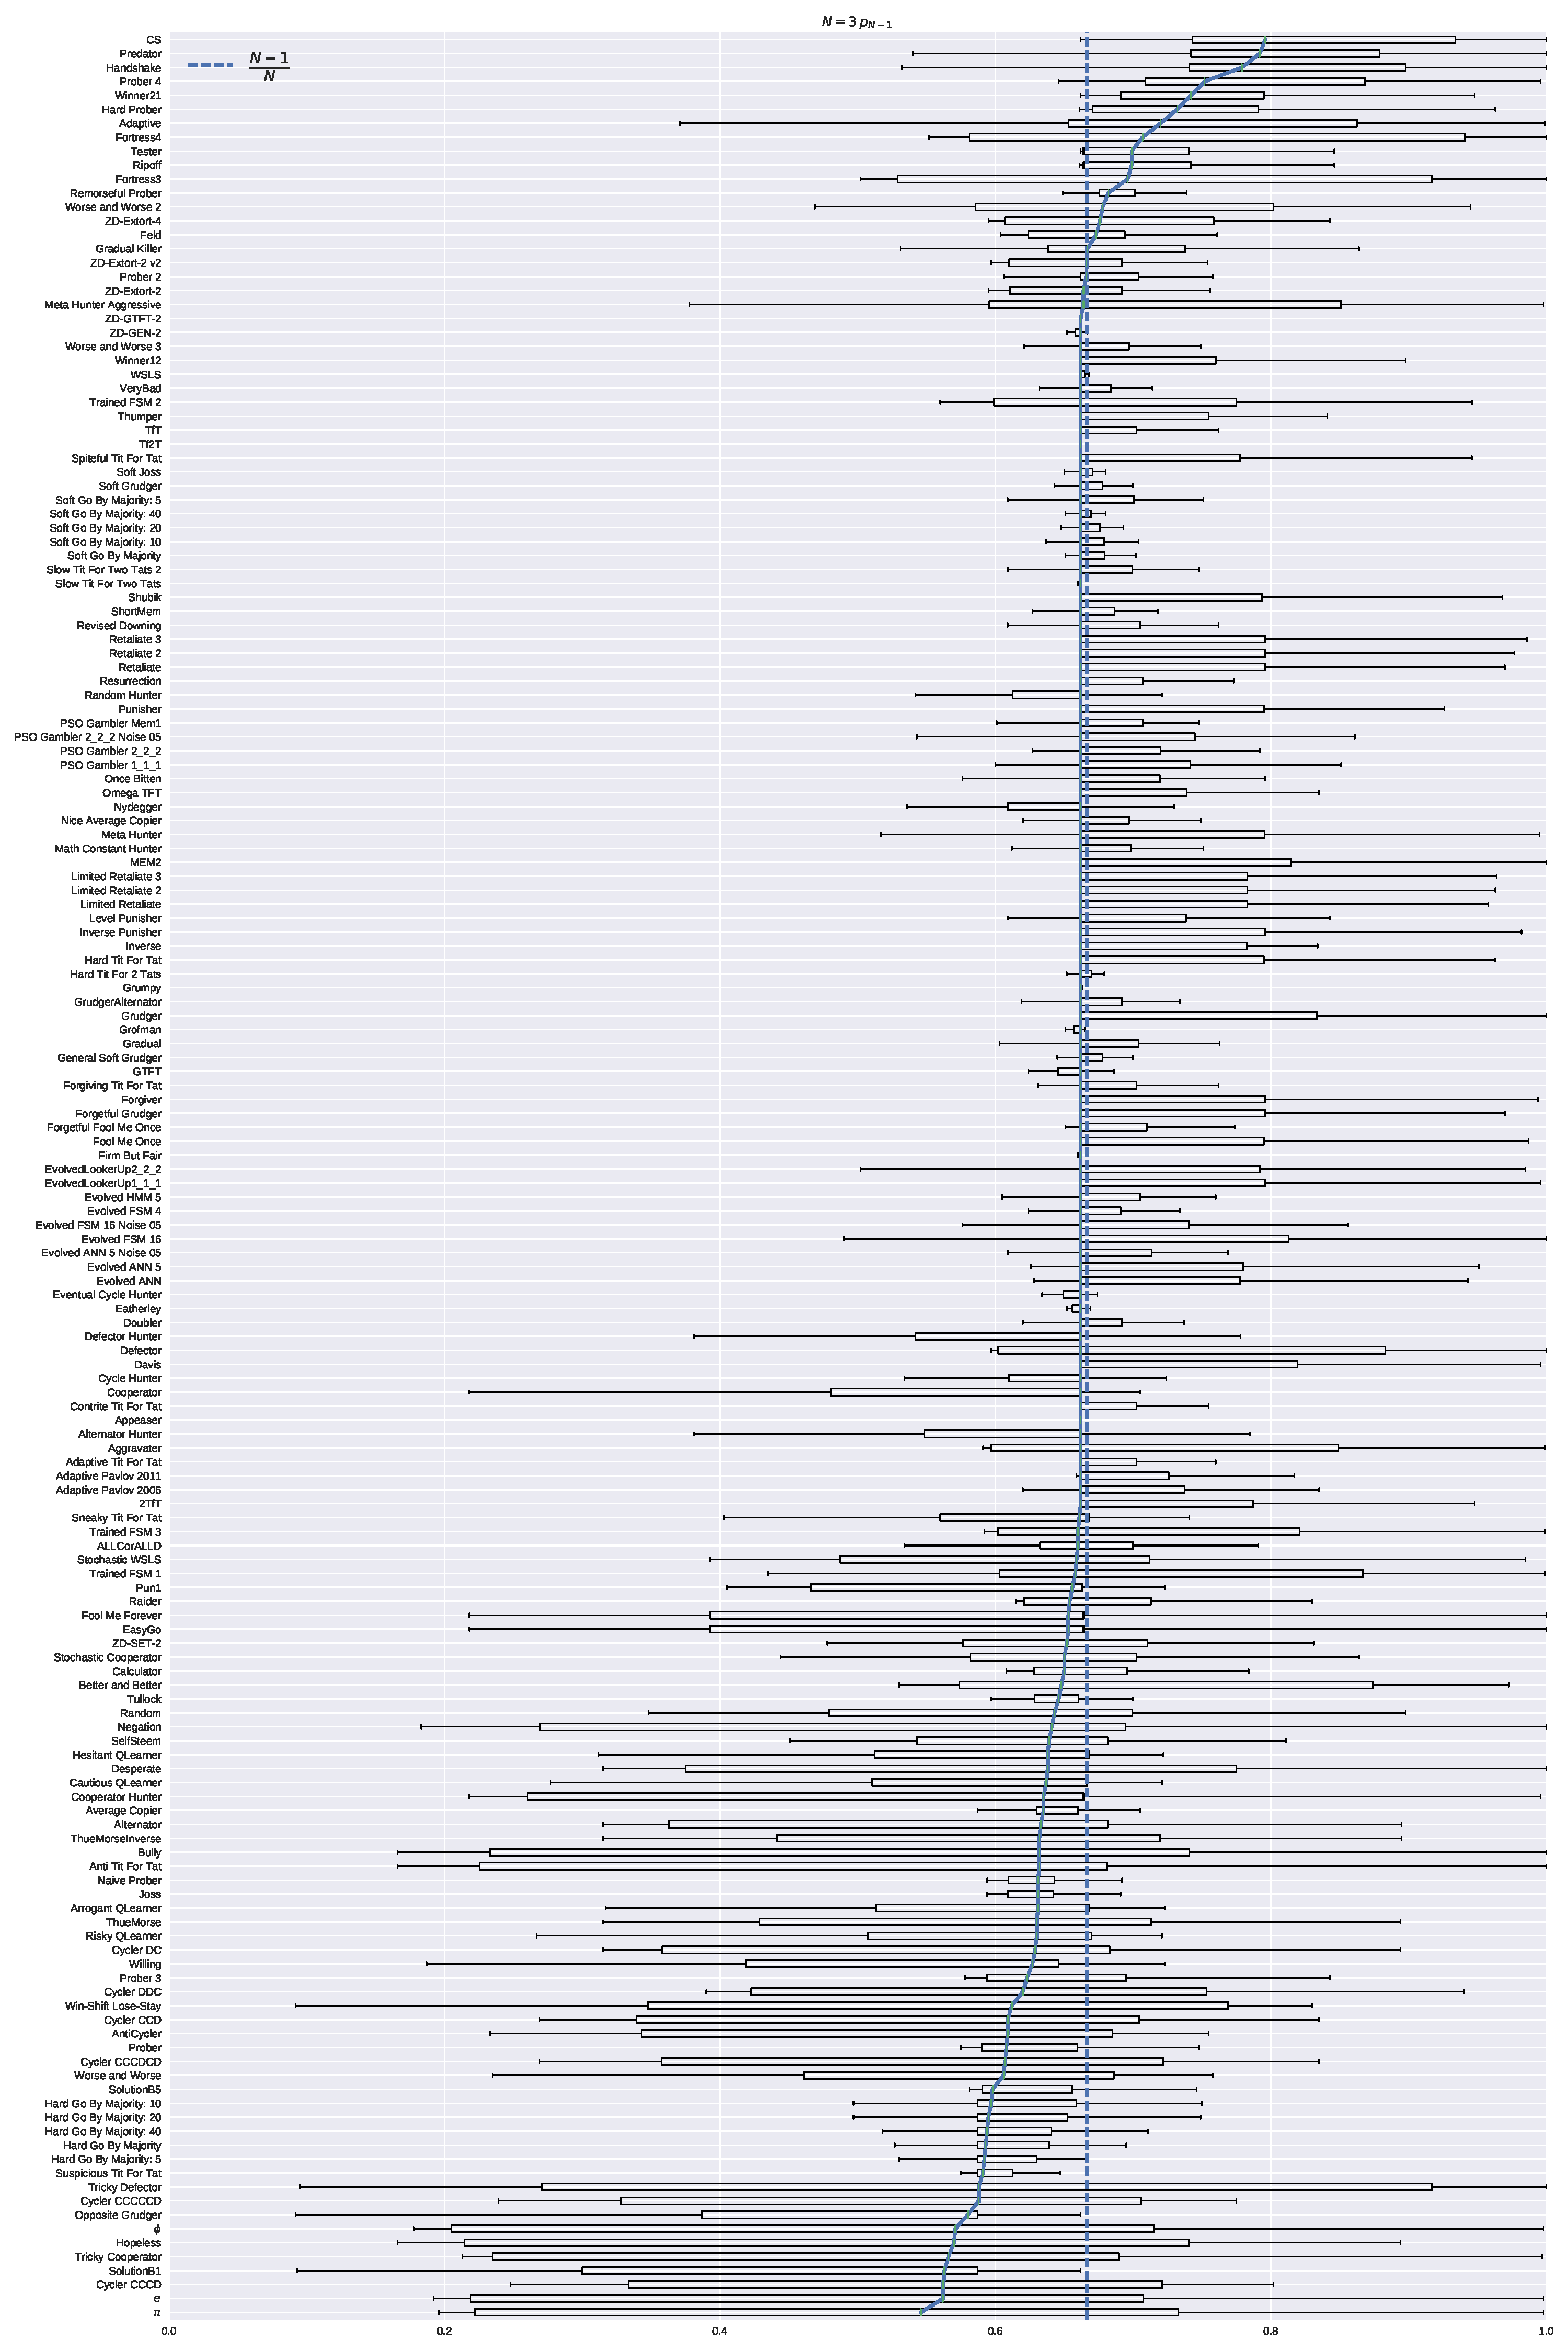
\includegraphics[width=\textwidth]{./img/boxplot_3_resist.pdf}
        \caption{\(N=2\)}
    \end{subfigure}%
    ~
    \begin{subfigure}[t]{.3\textwidth}
        \centering
        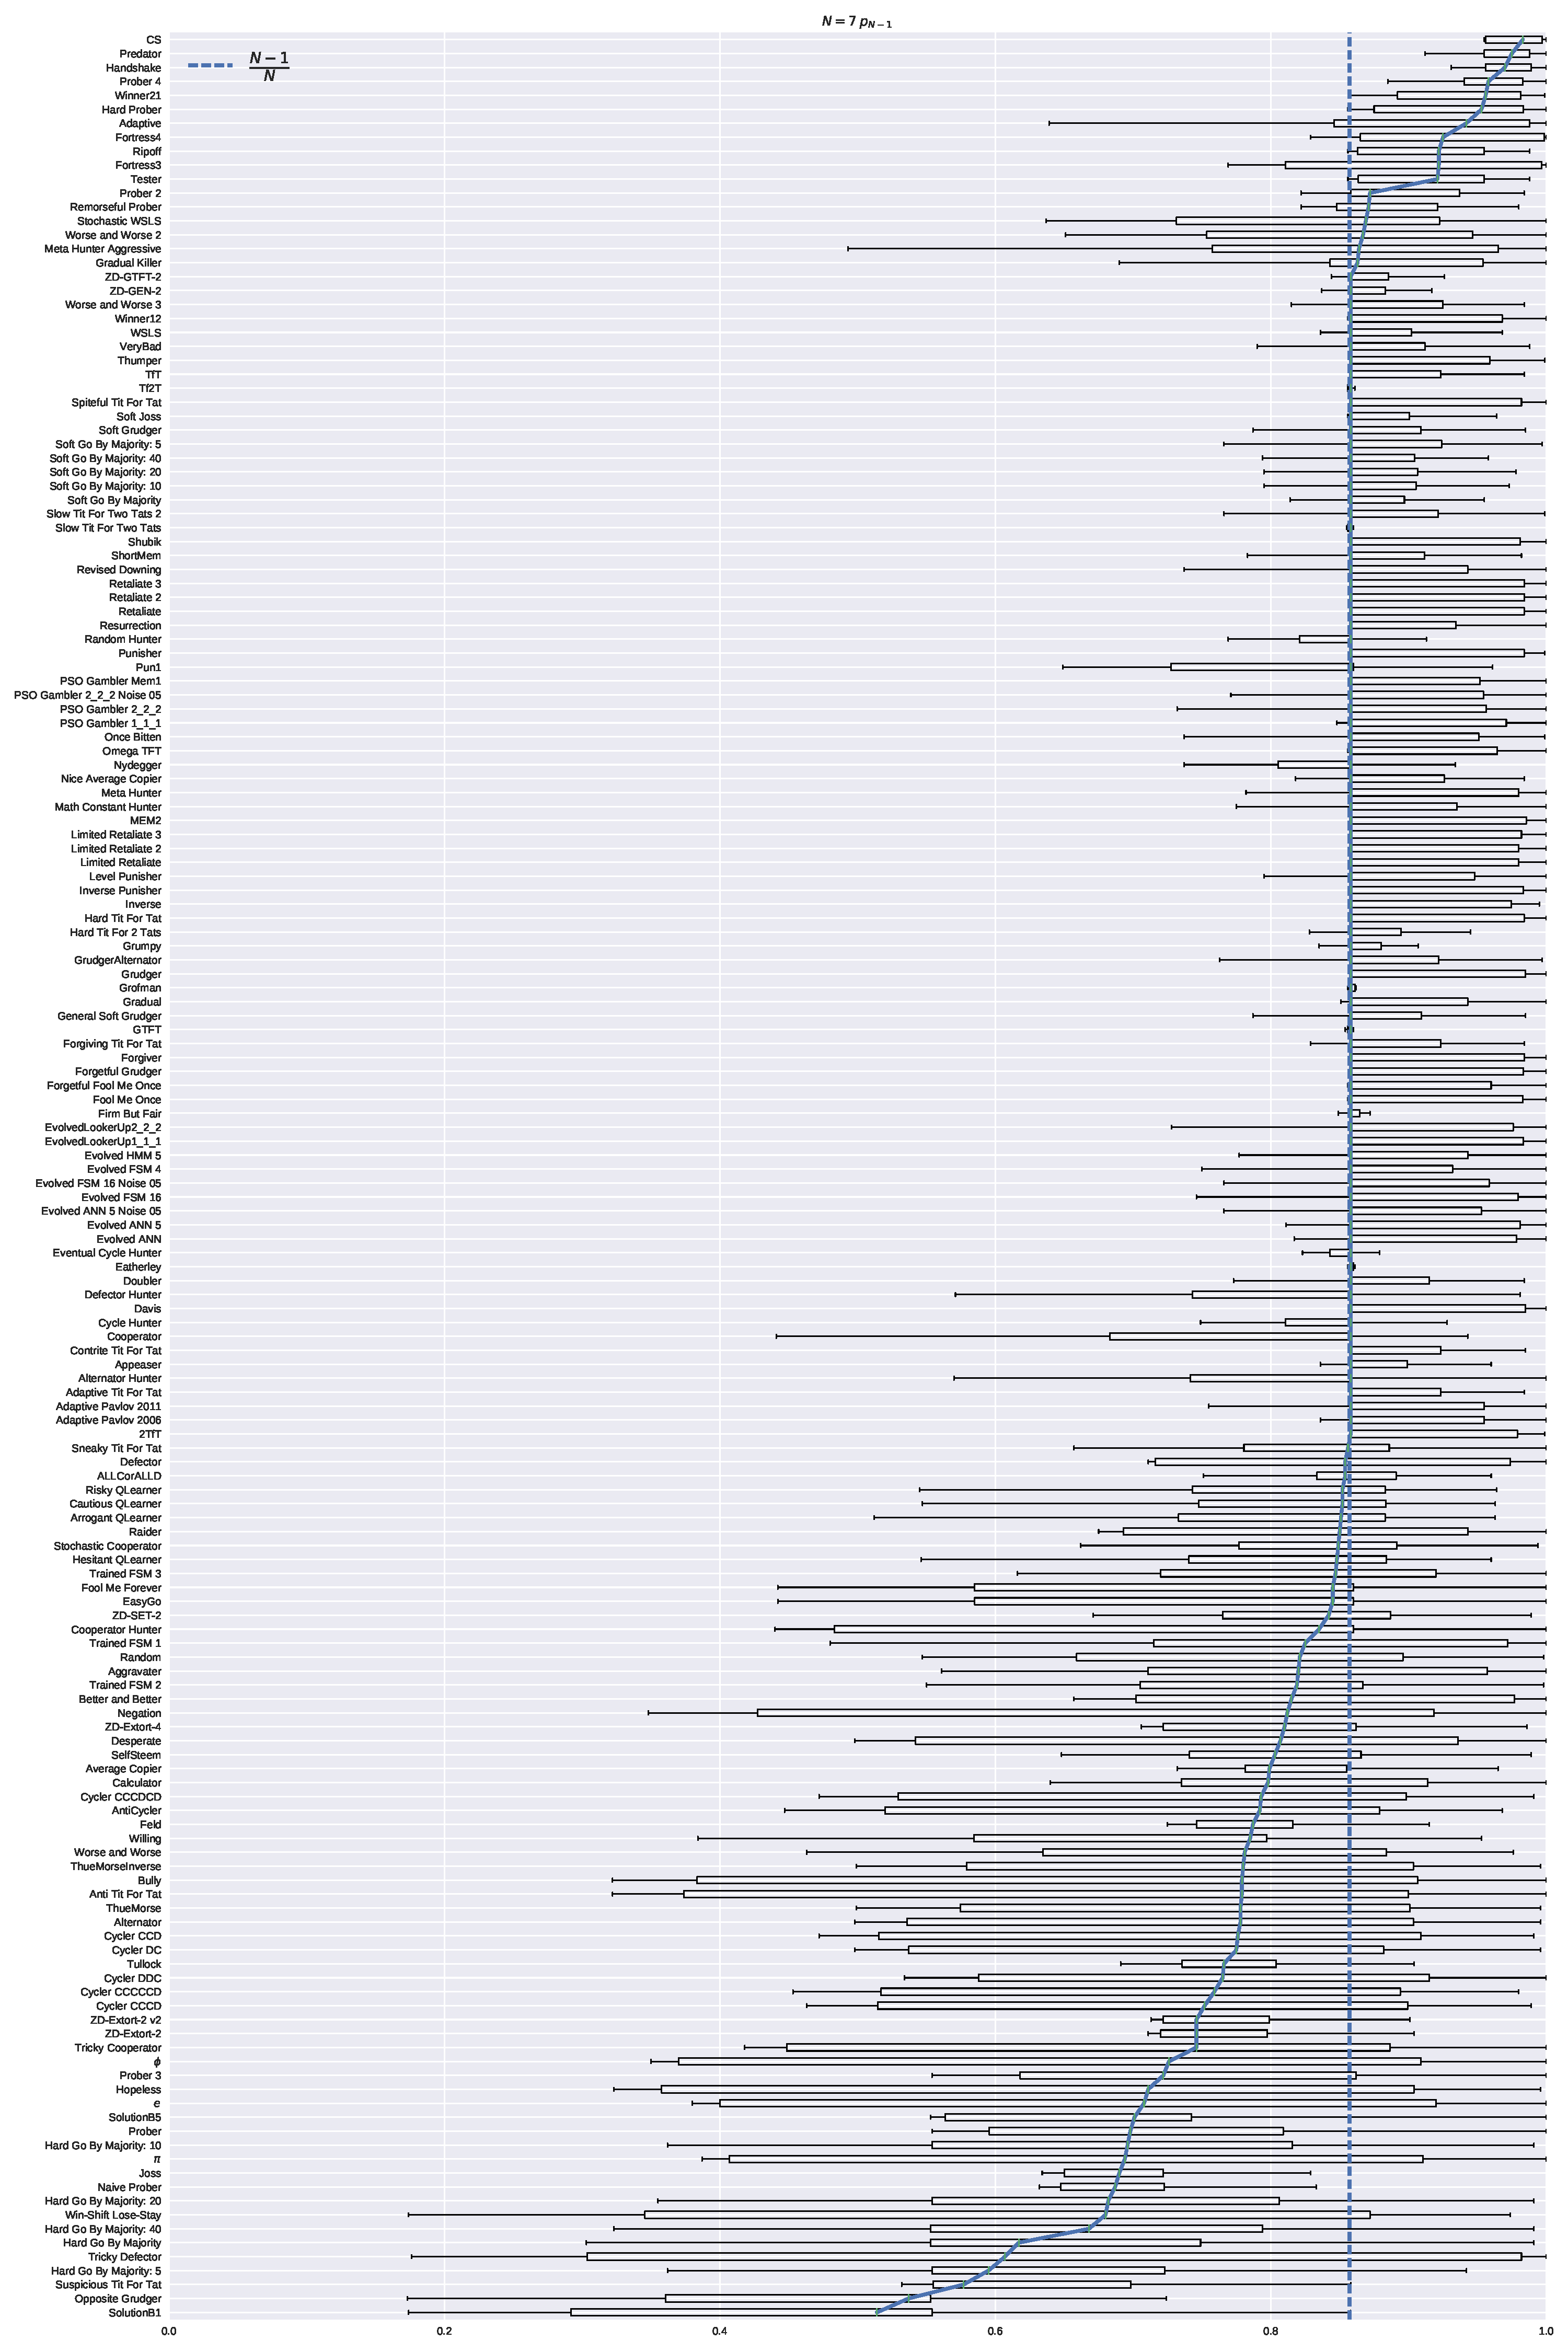
\includegraphics[width=\textwidth]{./img/boxplot_7_resist.pdf}
        \caption{\(N=7\)}
    \end{subfigure}%
    ~
    \begin{subfigure}[t]{.3\textwidth}
        \centering
        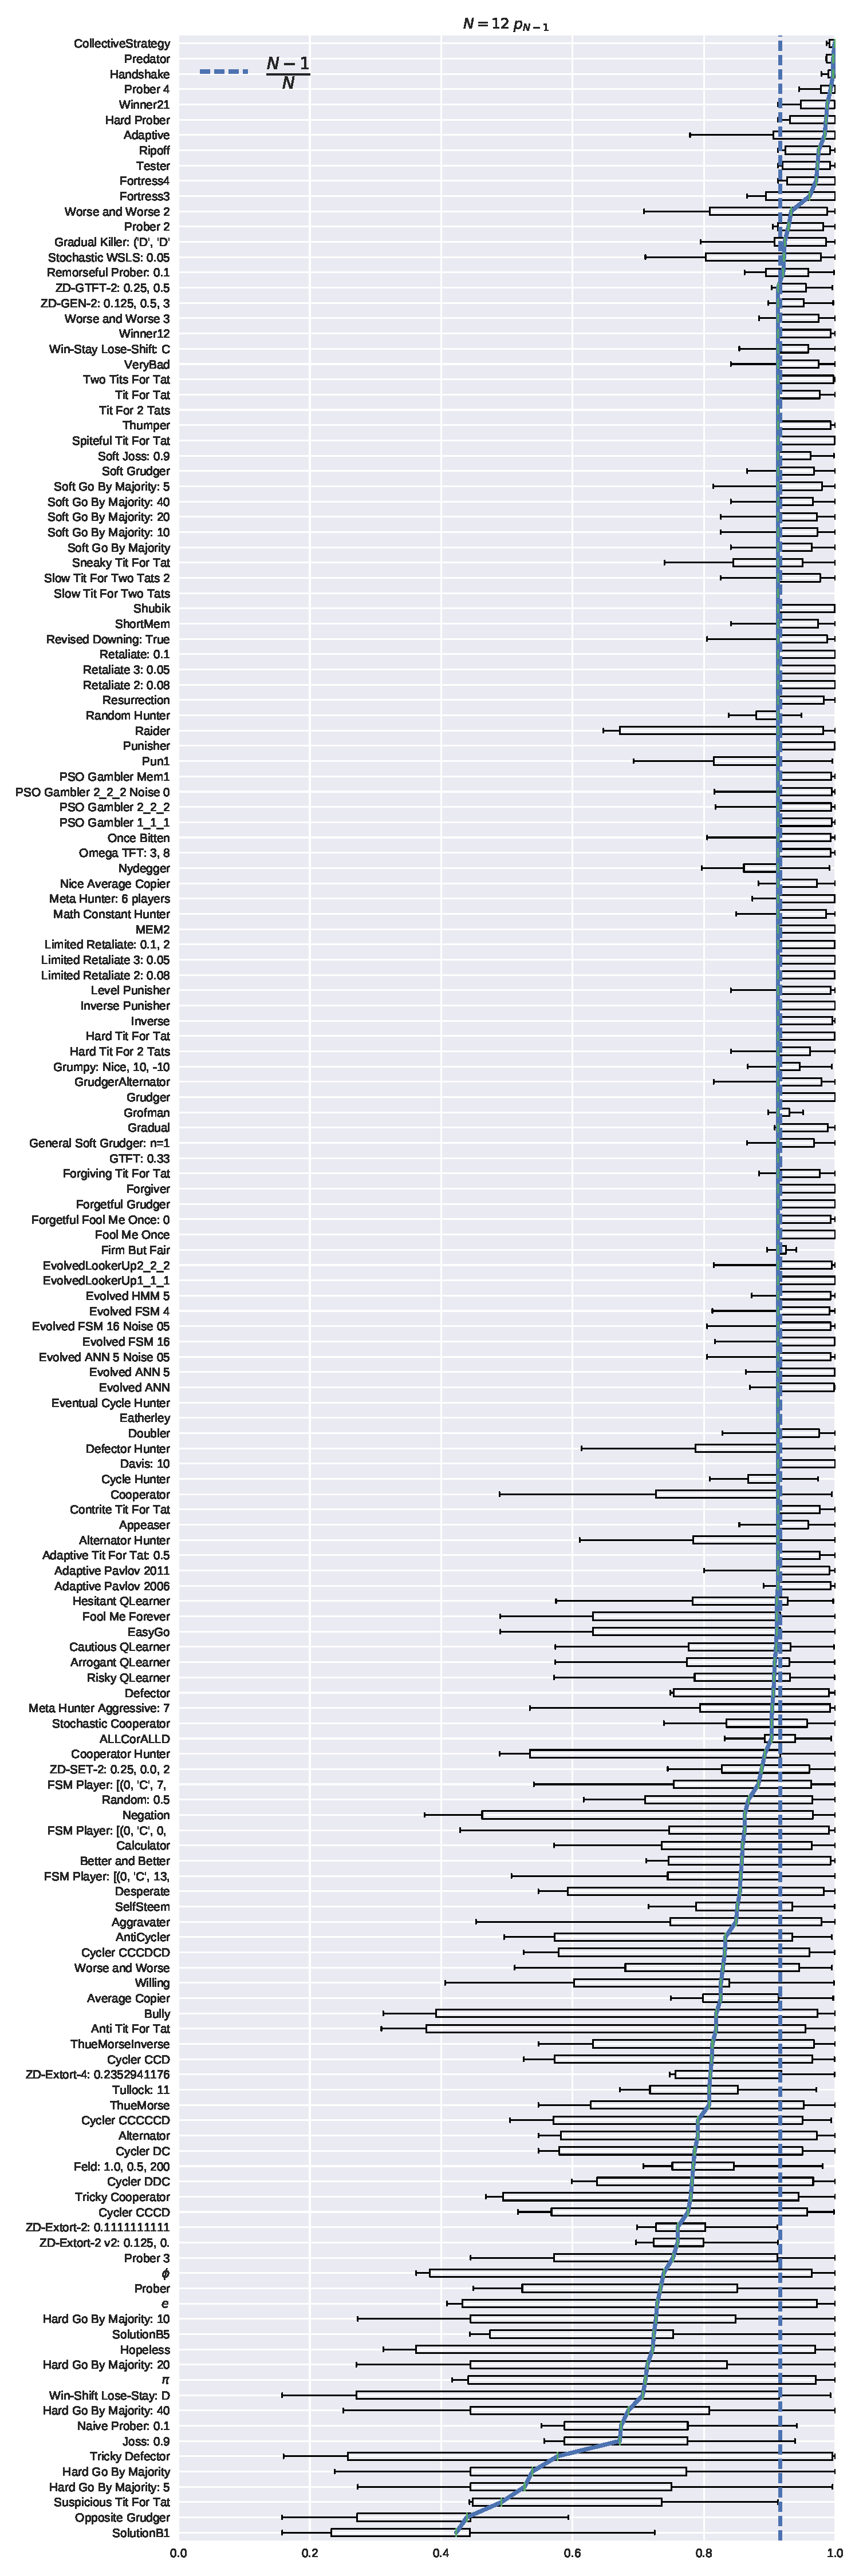
\includegraphics[width=\textwidth]{./img/boxplot_12_resist.pdf}
        \caption{\(N=12\)}
    \end{subfigure}%

    % TODO Replace N=12 with N=14 (when we have more data).
    \caption{Median probabilities \(x_{N-1}\) of all strategies as well as the
    neutral fixation probability}
    \label{fig:fixation_boxplot_resist}
\end{figure}

Table~\ref{tbl:top_five_resist} shows the top five strategies when ranked
according to \(x_{N-1}\) for \(N\in\{3, 7, 12\}\).
% TODO Change 12 to 14
Once again none of the short memory strategies from
Section~\ref{sec:two_individuals} perform well for high \(N\).

Three strategies have both high \(x_1\) and high \(x_{N-1}\):

\begin{itemize}
    \item Collective;
    \item Predator;
    \item Prober 4
\end{itemize}

However, Remorseful Prober, Worse and Worse 2 and Tester no longer do as well.
There are two strategies that are only top performers in \(x_{N-1}\):

\begin{itemize}
    \item Handshake: a slightly less aggressive version of the Collective
        strategy \cite{robson1989}. As long as the initial sequence is played
        then it cooperates. Thus it will do well in a population consisting of
        many members of itself: just as the Collective strategy does. However it
        is not aggressive enough to invade other populations.
    \item Winner 21: a strategy that makes it's decision deterministically based
        on 1 round of it's own strategy and 2 of the opponents strategy
        \cite{Mathieu2015}.
\end{itemize}
% TODO Revise this if need be for N=14

Interestingly none of these strategies are deterministic: this is explained by
the need of strategies to have a steady hand when interacting with their own
kind. In essence: acting stochastically increase the chance of friendly fire.


\begin{table}[!hbtp]
    \begin{subfigure}[t]{\textwidth}
        \centering
        \begin{tabular}{lrrl}
\toprule
    Player &  Mean $p_{N-1}$ &  Memory Depth & Stochastic \\
\midrule
        CS &        0.835859 &            \(\infty\) &      False \\
  Predator &        0.812129 &             9 &      False \\
       TF3 &        0.808736 &             1 &      False \\
 Handshake &        0.801356 &            \(\infty\) &      False \\
       TF2 &        0.795736 &             1 &      False \\
\bottomrule
\end{tabular}

        \caption{\(N=3\)}
    \end{subfigure}
    \begin{subfigure}[t]{\textwidth}
        \centering
        \begin{tabular}{lrrl}
\toprule
    Player &  Mean $p_{N-1}$ &  Memory Depth & Stochastic \\
\midrule
        CS &        0.976491 &            \(\infty\) &      False \\
       TF3 &        0.971405 &             1 &      False \\
       TF2 &        0.967712 &             1 &      False \\
  Predator &        0.967687 &             9 &      False \\
 Handshake &        0.954650 &            \(\infty\) &      False \\
\bottomrule
\end{tabular}

        \caption{\(N=7\)}
    \end{subfigure}
    \begin{subfigure}[t]{\textwidth}
        \centering
        \begin{tabular}{lrrl}
\toprule
   Player &  Mean $p_{N-1}$ &  Memory Depth & Stochastic \\
\midrule
       CS &        0.995564 &            \(\infty\) &      False \\
      TF3 &        0.993270 &             1 &      False \\
      TF2 &        0.991135 &             1 &      False \\
 Predator &        0.989816 &             9 &      False \\
 Prober 4 &        0.982129 &            \(\infty\) &      False \\
\bottomrule
\end{tabular}

        \caption{\(N=12\)}
    \end{subfigure}
    %TODO Change N=12 to N=14
    \caption{Properties of top five resistors}
    \label{tbl:top_five_resist}
\end{table}

It is evident through
Sections~\ref{sec:two_individuals},~\ref{sec:strong_invaders}
and~\ref{sec:strong_resistors} that performance of strategies not only depends
on the initial population distribution but also that there seems to be a
difference depending on whether or not \(N>2\). This will be explored further in
the next section.

\subsection{The effect of population size}\label{sec:population_size}

Figures~\ref{fig:ranks_v_size_invade},~\ref{fig:ranks_v_size_resist}
and~\ref{fig:ranks_v_size_coexist} show the median rank of each strategy against
population size. For all starting populations \(i\in\{1, N/2, N-1\}\) the ranks
of strategies are relatively stable across the different values of \(N>2\)
however for \(N=2\) there is a distinct difference. This confirms what has been
discussed in previous sections.

Tables~\ref{tbl:ranks_v_size_invade},~\ref{tbl:ranks_v_size_resist}
and~\ref{tbl:ranks_v_size_coexist} show the same information for the strategies
that rated high for \(N=2\) and \(N=12\).
% TODO Change to N=14?

\begin{figure}[!hbtp]
    \centering
    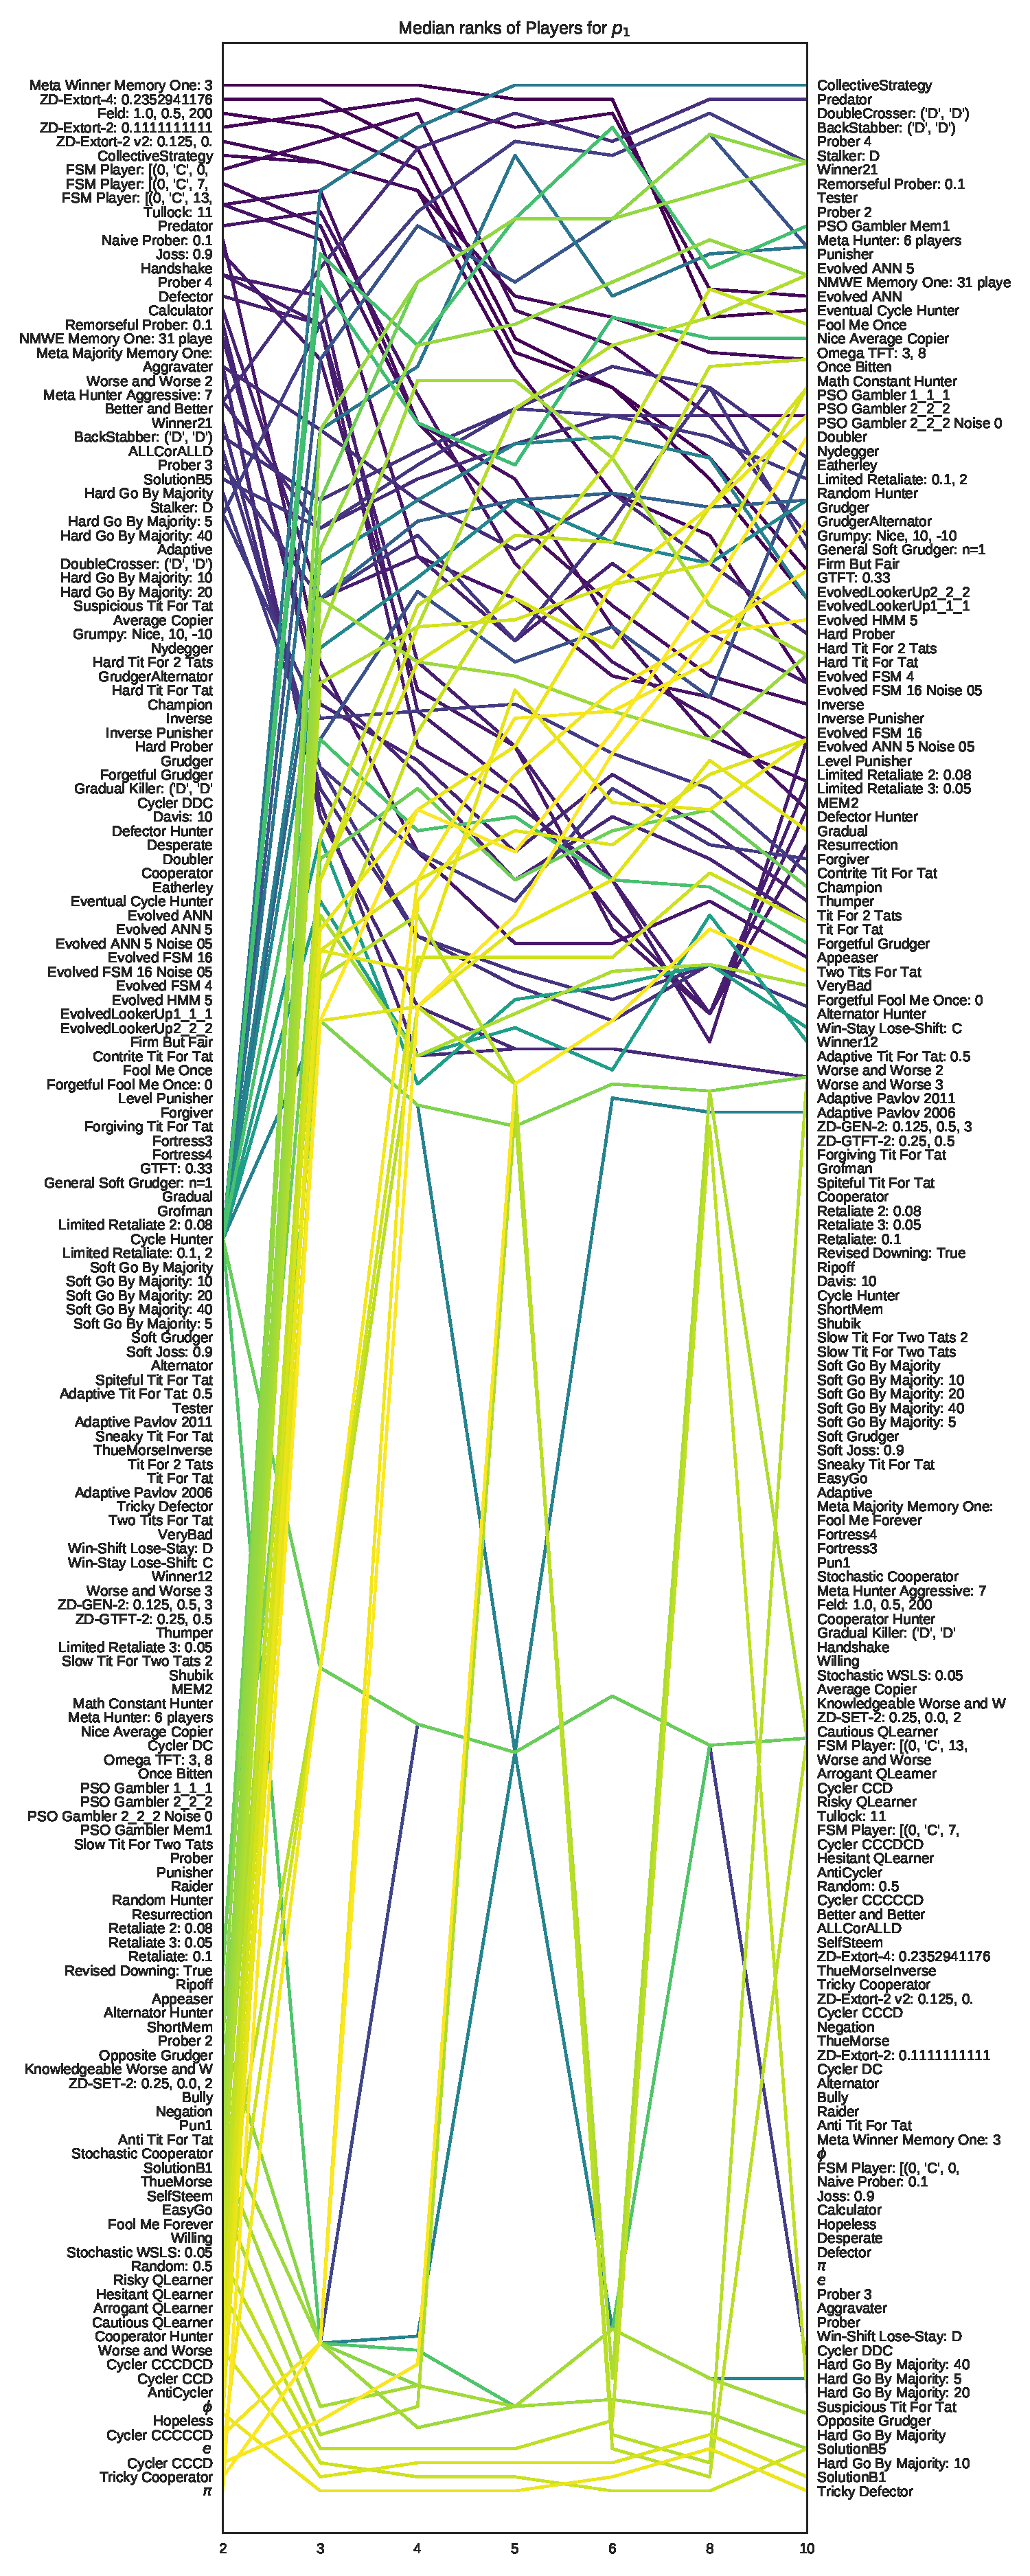
\includegraphics[height=.9\textheight]{./img/median_rank_vs_population_size_invade.pdf}
    \caption{Ranks of all strategies according to \(x_1\) for different
    population sizes}
    \label{fig:ranks_v_size_invade}
\end{figure}

\begin{table}[!hbtp]
    \centering
    \scriptsize
    \begin{tabular}{lrrrrrrrrrrrrr}
\toprule
               Player &     2 &     3 &     4 &     5 &      6 &      7 &      8 &      9 &     10 &     11 &     12 &     13 &     14 \\
\midrule
                   CS &   1.0 &   1.0 &   2.0 &   8.0 &    4.0 &    9.0 &   12.0 &   20.0 &   14.0 &   21.0 &   15.0 &   23.0 &   22.0 \\
        Trained FSM 1 &   2.0 &  29.0 &  55.0 &  71.0 &   67.0 &   57.0 &   54.0 &   71.0 &   60.0 &   68.0 &   53.0 &   59.0 &   53.0 \\
             Defector &   3.0 &  41.0 &  75.0 &  88.0 &   86.0 &   84.0 &   85.0 &   99.0 &   94.0 &  104.0 &   90.0 &  100.0 &   96.0 \\
           Aggravater &   4.0 &  48.0 &  88.0 &  98.0 &  101.0 &  102.0 &  107.0 &  112.0 &  111.0 &  114.0 &  113.0 &  113.0 &  116.0 \\
             Predator &   5.0 &   6.0 &  22.0 &  33.0 &   25.0 &   29.0 &   29.0 &   41.0 &   32.0 &   41.0 &   31.0 &   41.0 &   33.0 \\
       Evolved FSM 16 &  31.0 &  10.0 &   8.0 &   4.0 &    1.0 &    1.0 &    1.0 &    1.0 &    1.0 &    1.0 &    1.0 &    1.0 &    1.0 \\
    PSO Gambler 2\_2\_2 &  29.0 &  12.0 &   9.0 &   7.0 &    8.0 &    4.0 &    2.0 &    2.0 &    2.0 &    2.0 &    2.0 &    2.0 &    2.0 \\
          Evolved ANN &  20.0 &   9.0 &   6.0 &   5.0 &    7.0 &    5.0 &    3.0 &    3.0 &    3.0 &    3.0 &    3.0 &    3.0 &    3.0 \\
        Evolved ANN 5 &  21.0 &   8.0 &   5.0 &   6.0 &    6.0 &    3.0 &    5.0 &    4.0 &    4.0 &    4.0 &    5.0 &    4.0 &    4.0 \\
 EvolvedLookerUp2\_2\_2 &  33.0 &  15.0 &  11.0 &  10.0 &    9.0 &    8.0 &    6.0 &    6.0 &    5.0 &    5.0 &    4.0 &    5.0 &    5.0 \\
\bottomrule
\end{tabular}

    \caption{Ranks of some strategies according to \(x_1\) for different
    population sizes}
    \label{tbl:ranks_v_size_invade}
\end{table}

\begin{figure}[!hbtp]
    \centering
    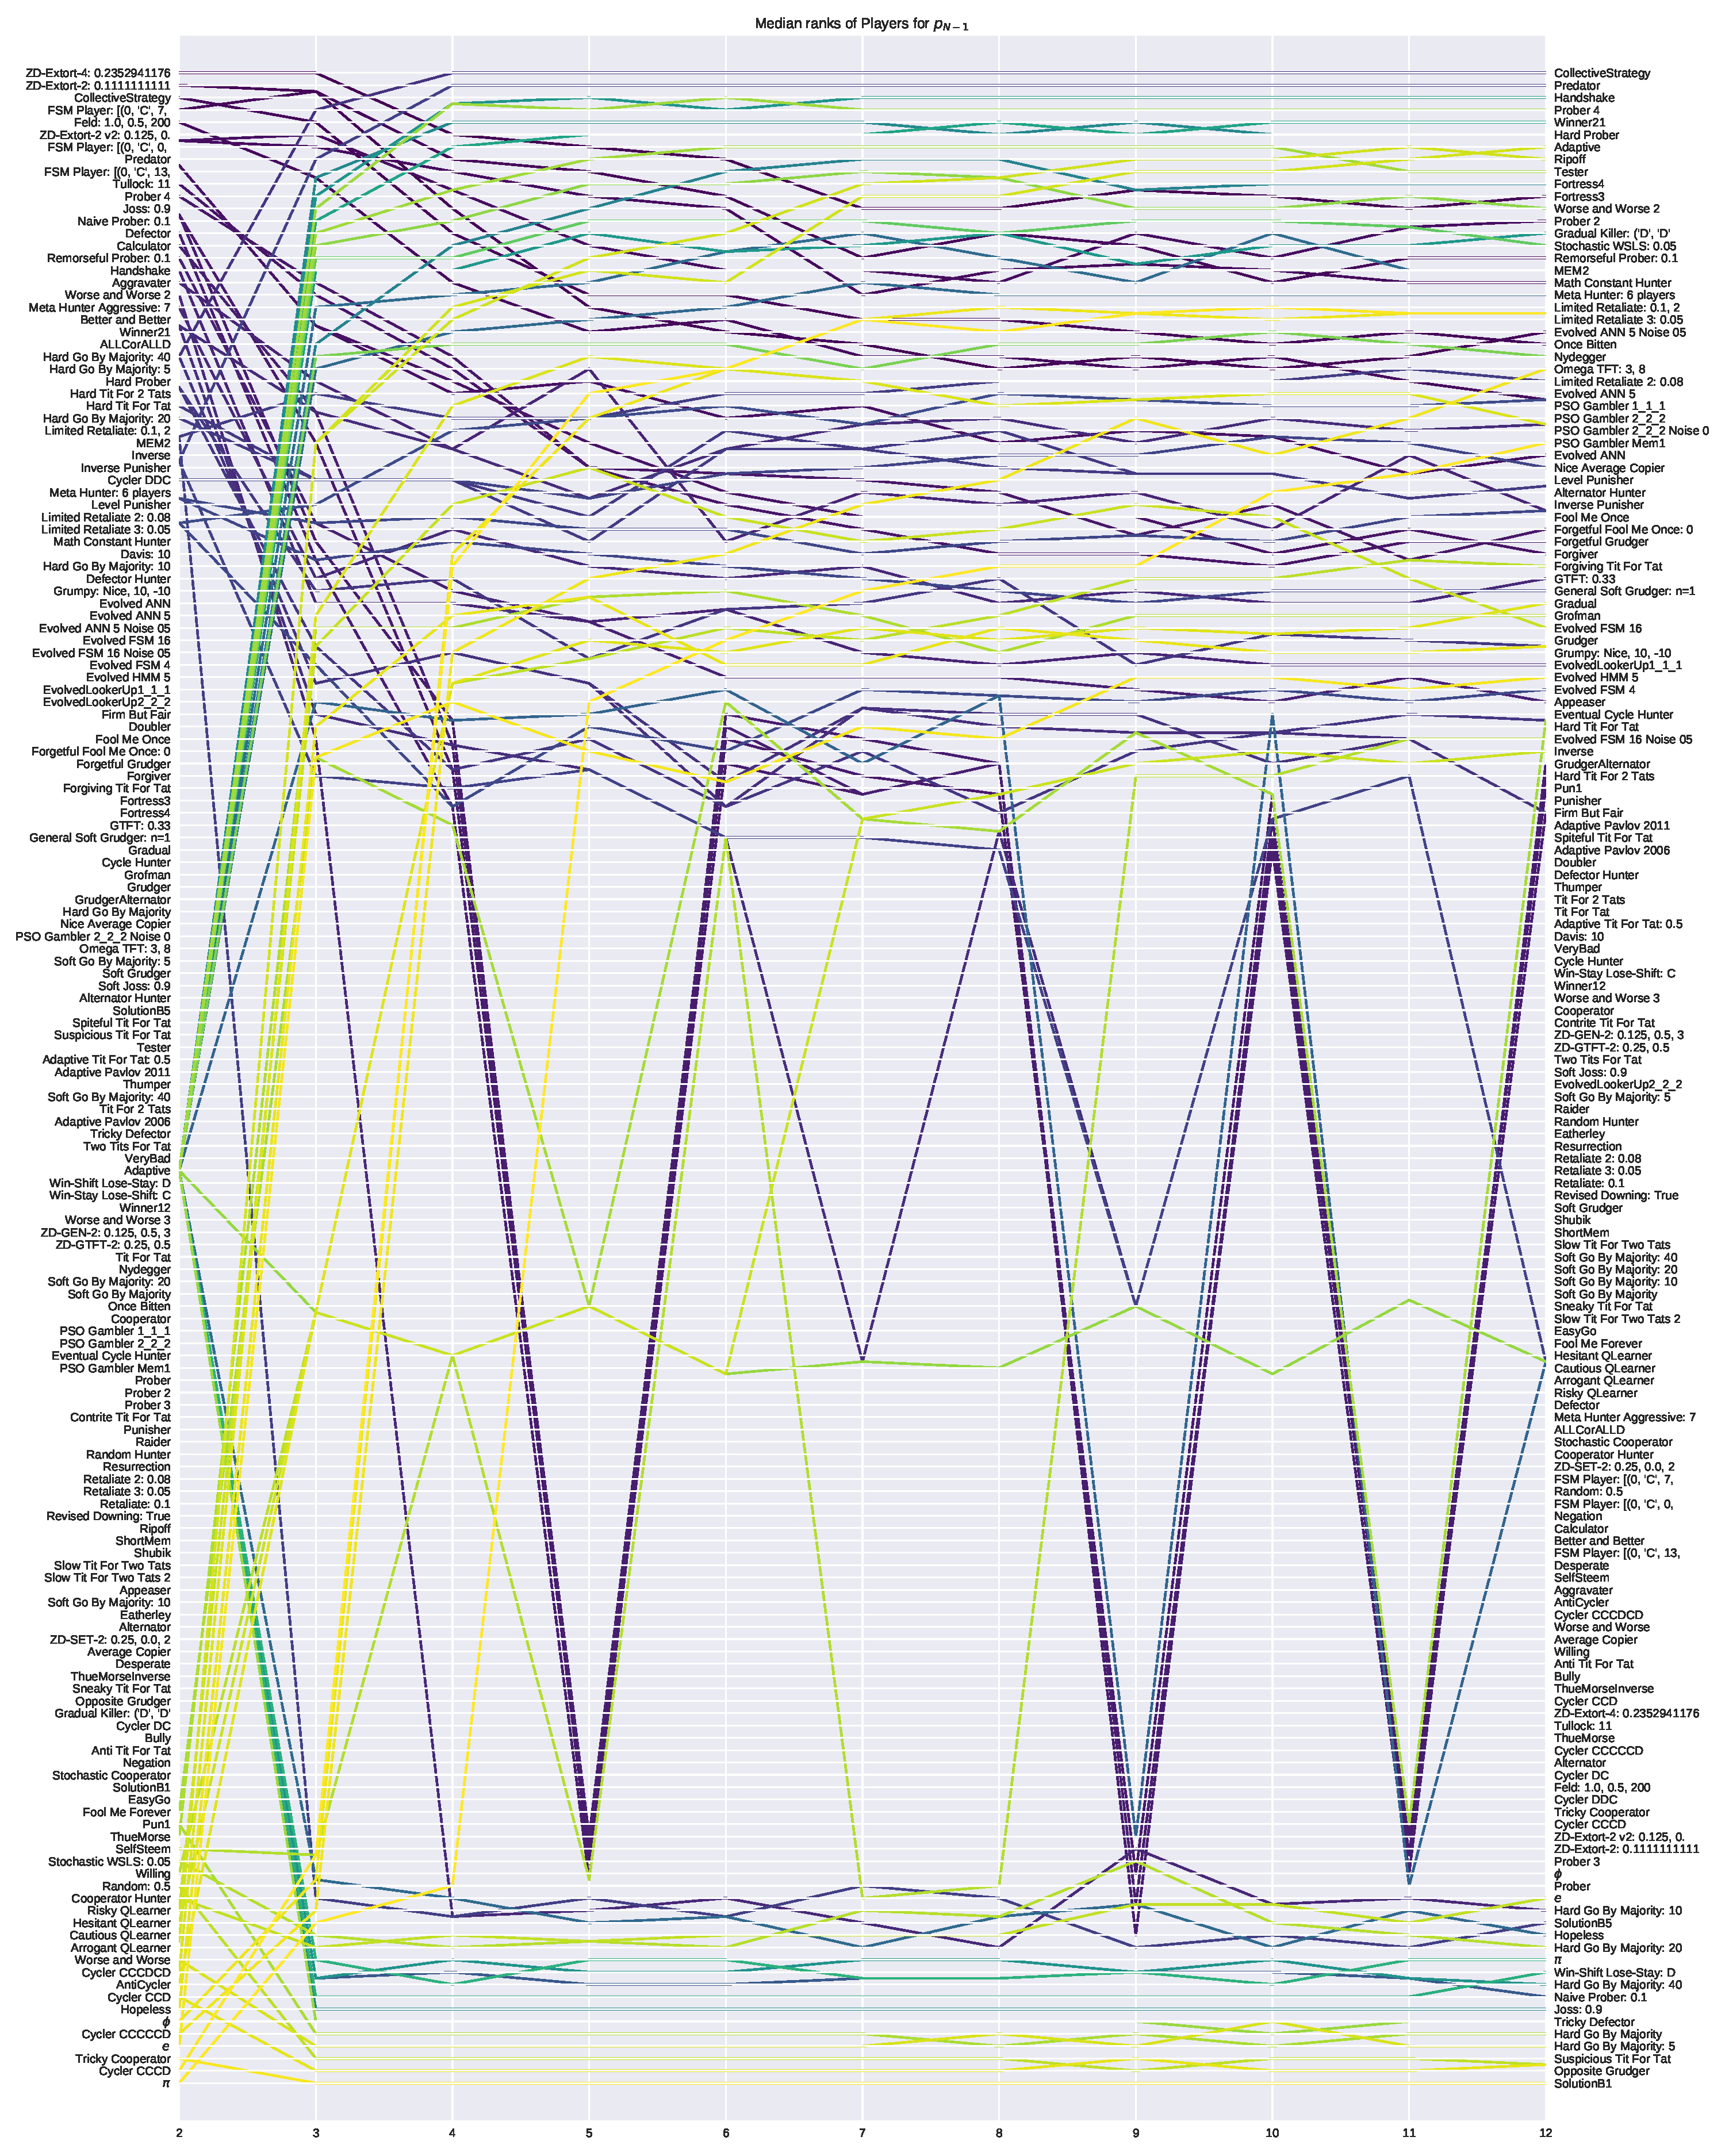
\includegraphics[height=.9\textheight]{./img/median_rank_vs_population_size_resist.pdf}
    \caption{Ranks of all strategies according to \(x_{N-1}\) for different
    population sizes}
    \label{fig:ranks_v_size_resist}
\end{figure}

\begin{table}[!hbtp]
    \centering
    \scriptsize
    \begin{tabular}{lrrrrrrrrrrr}
\toprule
        Player &     2 &      3 &      4 &      5 &      6 &      7 &      8 &      9 &     10 &     11 &     12 \\
\midrule
   ZD-Extort-4 &   1.0 &   10.0 &  103.0 &  108.0 &  118.0 &  120.5 &  123.5 &  122.0 &  124.5 &  129.0 &  128.5 \\
            CS &   2.0 &    1.0 &    1.0 &    1.0 &    1.0 &    2.0 &    2.0 &    2.0 &    2.0 &   48.5 &   49.5 \\
 Trained FSM 3 &   3.0 &  105.5 &  103.0 &  106.5 &  112.5 &  114.0 &  115.0 &  110.0 &  112.0 &  110.0 &  114.0 \\
          Feld &   4.5 &    6.0 &    6.0 &   99.5 &  103.0 &   99.0 &  108.0 &  107.0 &  103.0 &  109.0 &  113.0 \\
   ZD-Extort-2 &   4.5 &   13.5 &  112.0 &  113.5 &  119.5 &  123.0 &  125.0 &  126.5 &  134.0 &  130.0 &  142.5 \\
            CS &   3.0 &    1.0 &    1.0 &    1.0 &    1.0 &    1.0 &    1.0 &    1.0 &    1.0 &    1.0 &    1.0 \\
     Handshake &  17.0 &    3.0 &    3.0 &    3.0 &    3.0 &    3.0 &    3.0 &    2.0 &    3.0 &    3.0 &    2.5 \\
      Predator &   8.0 &    2.0 &    2.0 &    2.0 &    2.0 &    2.0 &    2.0 &    3.0 &    2.0 &    2.0 &    2.5 \\
      Prober 4 &  11.0 &    4.0 &    4.0 &    4.0 &    4.0 &    4.0 &    5.0 &    4.0 &    6.0 &    4.0 &    4.0 \\
      Winner21 &  22.0 &    5.0 &    5.0 &    5.0 &    5.0 &    5.0 &    4.0 &    5.0 &    4.0 &    5.0 &    5.0 \\
\bottomrule
\end{tabular}

    \caption{Ranks of some strategies according to \(x_{N-1}\) for different
    population sizes}
    \label{tbl:ranks_v_size_resist}
\end{table}

\begin{figure}[!hbtp]
    \centering
    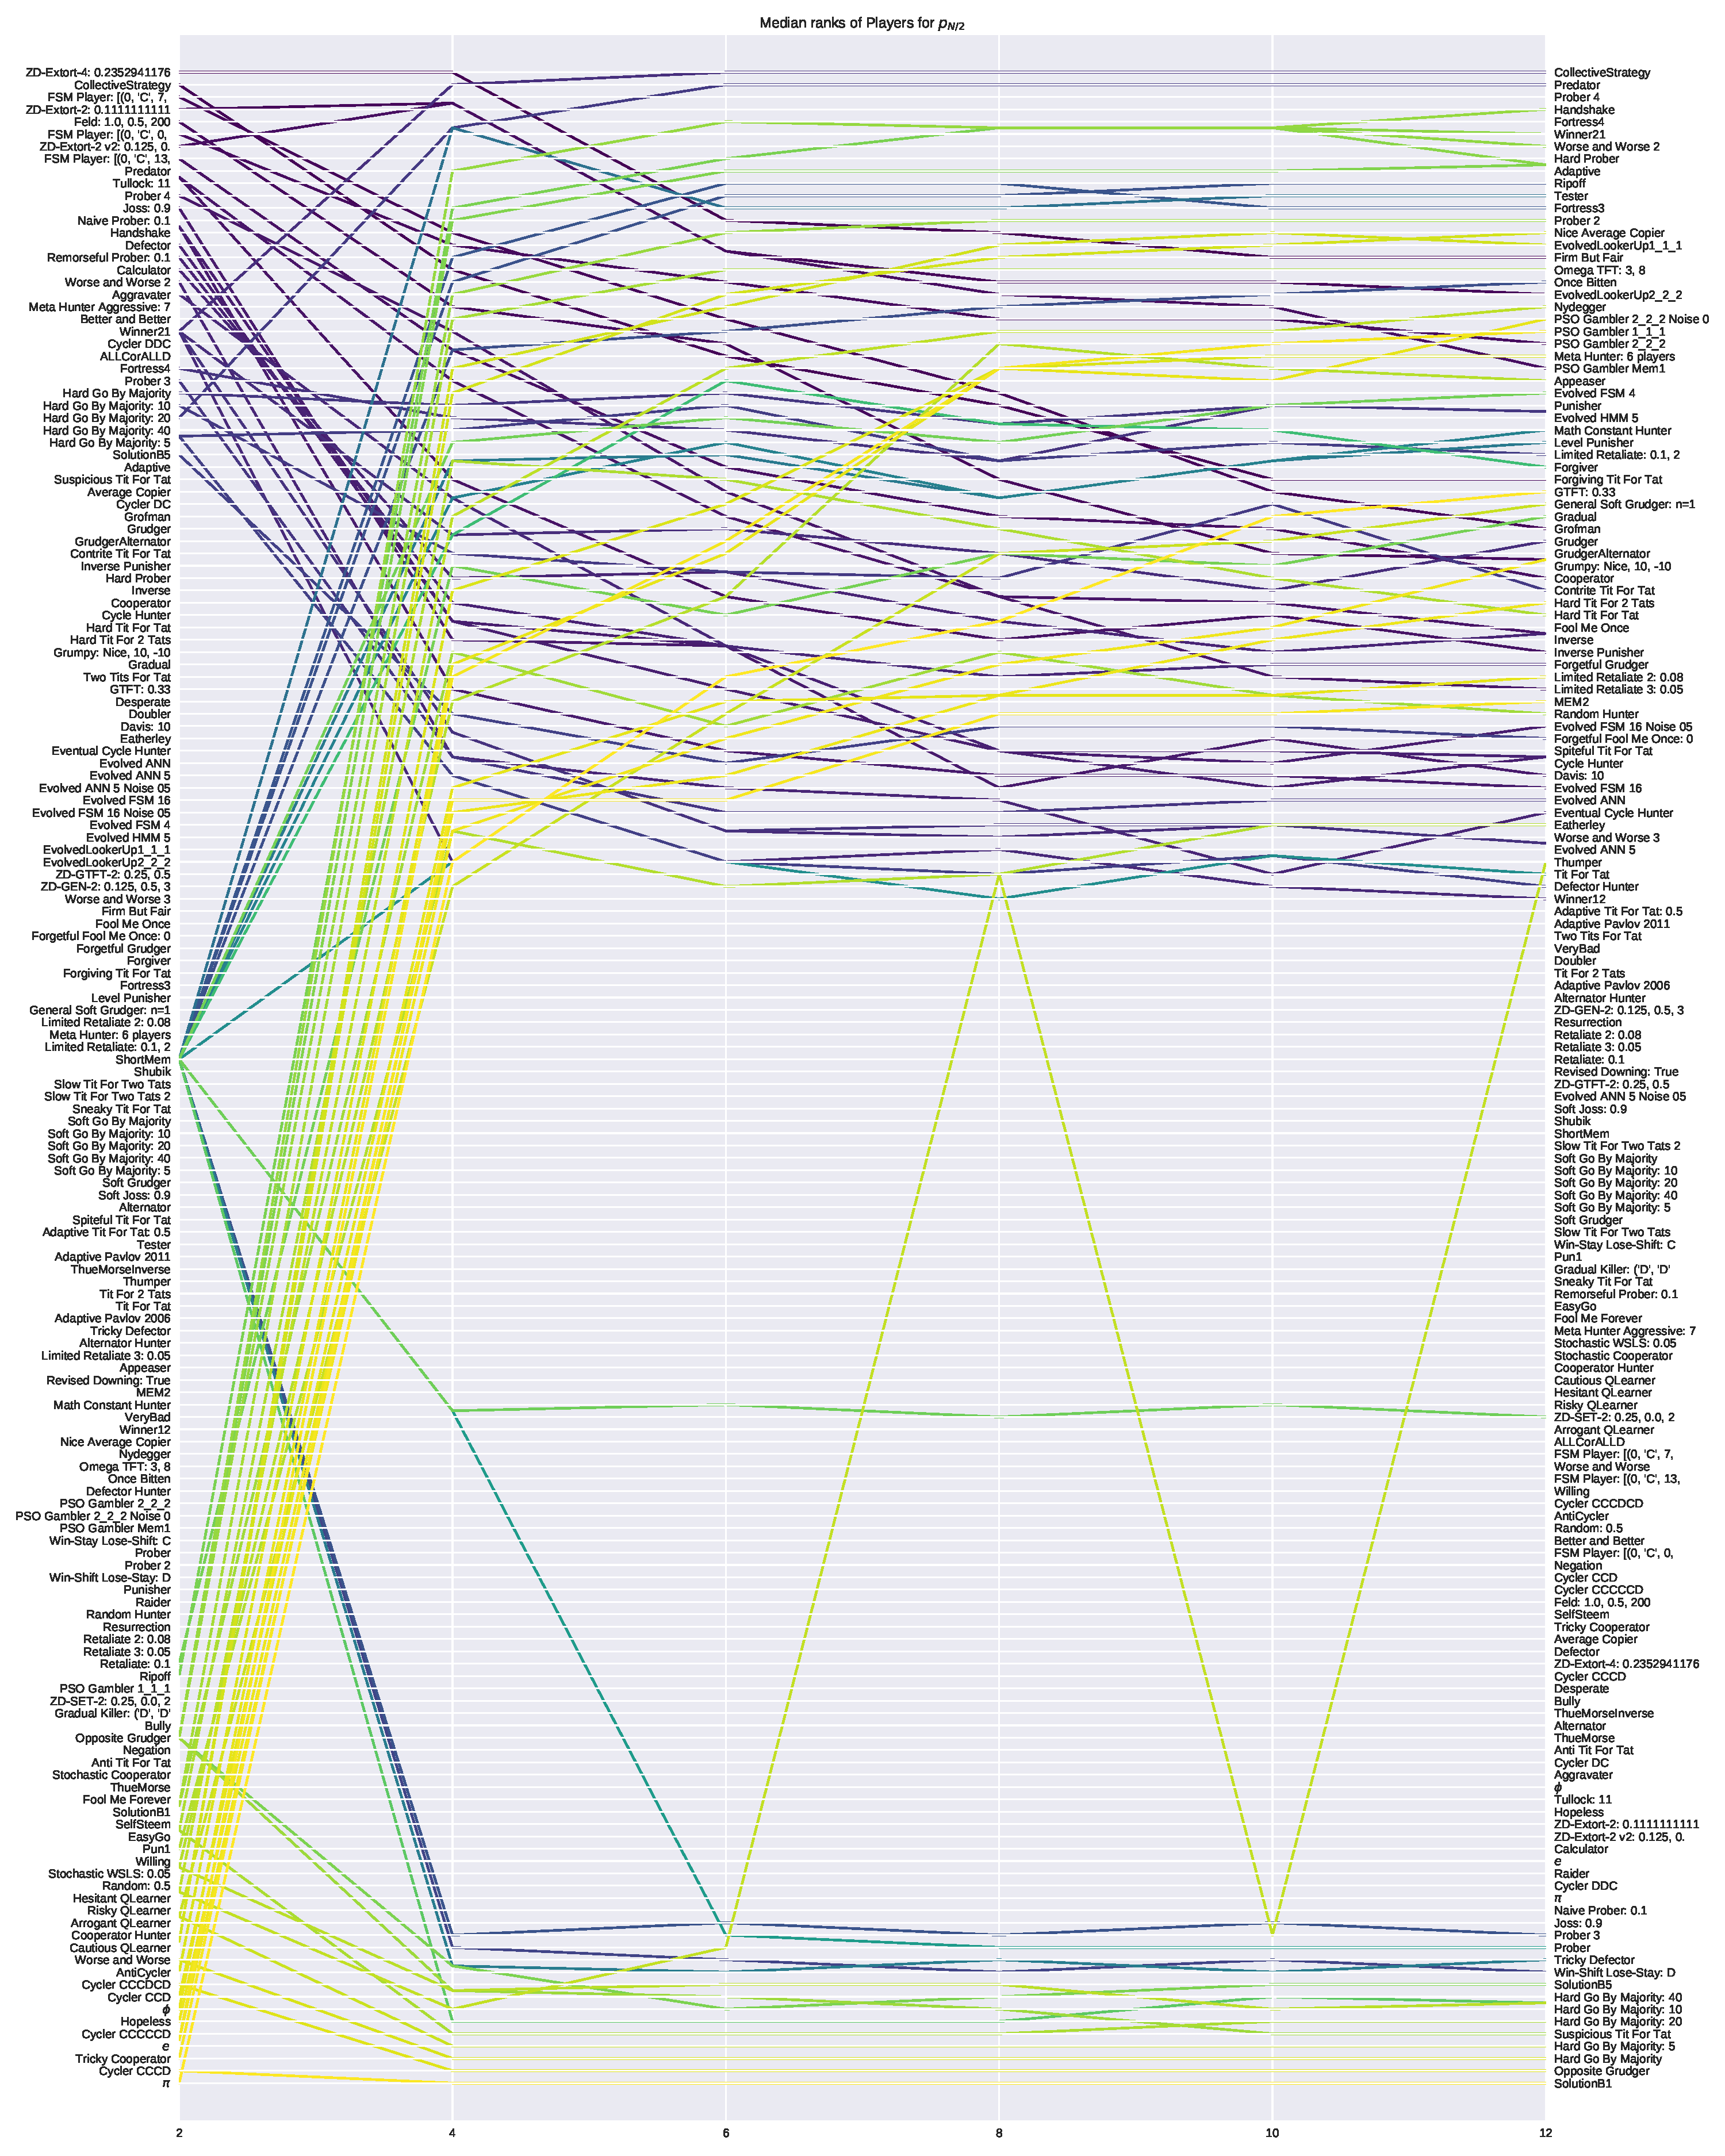
\includegraphics[height=.9\textheight]{./img/median_rank_vs_population_size_coexist.pdf}
    \caption{Ranks of all strategies according to \(x_{N/2}\) for different
    population sizes}
    \label{fig:ranks_v_size_coexist}
\end{figure}

\begin{table}[!hbtp]
    \centering
    \scriptsize
    \begin{tabular}{lrrrrrr}
\toprule
                                            Player &     2 &      4 &      6 &      8 &     10 &     12 \\
\midrule
         ZD-Extort-4: 0.23529411764705882, 0.25, 1 &   1.0 &  103.0 &  118.0 &  123.5 &  124.5 &  128.5 \\
                                CollectiveStrategy &   2.0 &    1.0 &    1.0 &    2.0 &    2.0 &   49.5 \\
 FSM Player: [(0, 'C', 7, 'C'), (0, 'D', 1, 'C'... &   3.0 &  103.0 &  112.5 &  115.0 &  112.0 &  114.0 \\
                               Feld: 1.0, 0.5, 200 &   4.5 &    6.0 &  103.0 &  108.0 &  103.0 &  113.0 \\
              ZD-Extort-2: 0.1111111111111111, 0.5 &   4.5 &  112.0 &  119.5 &  125.0 &  134.0 &  142.5 \\
                                CollectiveStrategy &   2.0 &    1.0 &    1.0 &    1.0 &    1.0 &    1.0 \\
                                          Predator &   9.0 &    2.0 &    2.0 &    2.0 &    2.0 &    2.0 \\
                                          Prober 4 &  11.0 &    3.0 &    3.0 &    3.0 &    3.0 &    3.0 \\
                                         Handshake &  14.5 &    4.0 &    4.0 &    4.0 &    4.0 &    4.0 \\
                                         Fortress4 &  29.0 &    8.5 &    8.0 &    7.0 &    5.0 &    5.0 \\
\bottomrule
\end{tabular}

    \caption{Ranks of some strategies according to \(x_{N/2}\) for different
    population sizes}
    \label{tbl:ranks_v_size_coexist}
\end{table}

Tables~\ref{tbl:correlation_coeficients_invade},~\ref{tbl:correlation_coeficients_resist}
and~\ref{tbl:correlation_coeficients_coexist} show the correlation coefficients
of the ranks in of strategies in differing population size. This is shown
graphically in Figure~\ref{fig:correlation_coefficients}. It is immediate to
note that how well a strategy performs in any Moran process for \(N>2\) has
little to do with the performance for \(N=2\). This illustrates why the strong
performance of zero determinant strategies predicted in \cite{Press2012} does
not extend to larger populations. This was discussed theoretically in
\cite{Adami2013} however not observed empirically at the scale presented here.


\begin{table}[!hbtp]
    \centering
    \begin{subfigure}{\textwidth}
        \centering
        \begin{tabular}{lrrrrrrrrr}
\toprule
N &    2  &    3  &    4  &    5  &    6  &    7  &    8  &    9  &    10 \\
\midrule
2  &  1.00 &  0.44 &  0.26 &  0.17 &  0.15 &  0.12 &  0.08 &  0.07 &  0.08 \\
3  &  0.44 &  1.00 &  0.92 &  0.87 &  0.87 &  0.86 &  0.83 &  0.83 &  0.84 \\
4  &  0.26 &  0.92 &  1.00 &  0.97 &  0.96 &  0.97 &  0.95 &  0.95 &  0.95 \\
5  &  0.17 &  0.87 &  0.97 &  1.00 &  0.98 &  0.99 &  0.97 &  0.98 &  0.98 \\
6  &  0.15 &  0.87 &  0.96 &  0.98 &  1.00 &  0.99 &  0.97 &  0.97 &  0.98 \\
7  &  0.12 &  0.86 &  0.97 &  0.99 &  0.99 &  1.00 &  0.98 &  0.98 &  0.99 \\
8  &  0.08 &  0.83 &  0.95 &  0.97 &  0.97 &  0.98 &  1.00 &  0.97 &  0.98 \\
9  &  0.07 &  0.83 &  0.95 &  0.98 &  0.97 &  0.98 &  0.97 &  1.00 &  0.99 \\
10 &  0.08 &  0.84 &  0.95 &  0.98 &  0.98 &  0.99 &  0.98 &  0.99 &  1.00 \\
\bottomrule
\end{tabular}

        \caption{Correlation coefficients for ranks for invasion}
        \label{tbl:correlation_coeficients_invade}
    \end{subfigure}%

    \begin{subfigure}{\textwidth}
        \centering
        \begin{tabular}{lrrrrrrrrrr}
\toprule
N &    2  &    3  &    4  &    5  &    6  &    7  &    8  &    9  &    10 &    12 \\
\midrule
2  &  1.00 &  0.61 &  0.42 &  0.29 &  0.35 &  0.34 &  0.34 &  0.20 &  0.30 &  0.27 \\
3  &  0.61 &  1.00 &  0.91 &  0.81 &  0.87 &  0.87 &  0.87 &  0.76 &  0.85 &  0.83 \\
4  &  0.42 &  0.91 &  1.00 &  0.93 &  0.98 &  0.97 &  0.97 &  0.89 &  0.96 &  0.95 \\
5  &  0.29 &  0.81 &  0.93 &  1.00 &  0.93 &  0.94 &  0.94 &  0.96 &  0.93 &  0.92 \\
6  &  0.35 &  0.87 &  0.98 &  0.93 &  1.00 &  0.98 &  0.98 &  0.92 &  0.99 &  0.99 \\
7  &  0.34 &  0.87 &  0.97 &  0.94 &  0.98 &  1.00 &  1.00 &  0.92 &  0.99 &  0.98 \\
8  &  0.34 &  0.87 &  0.97 &  0.94 &  0.98 &  1.00 &  1.00 &  0.91 &  0.98 &  0.98 \\
9  &  0.20 &  0.76 &  0.89 &  0.96 &  0.92 &  0.92 &  0.91 &  1.00 &  0.93 &  0.93 \\
10 &  0.30 &  0.85 &  0.96 &  0.93 &  0.99 &  0.99 &  0.98 &  0.93 &  1.00 &  1.00 \\
12 &  0.27 &  0.83 &  0.95 &  0.92 &  0.99 &  0.98 &  0.98 &  0.93 &  1.00 &  1.00 \\
\bottomrule
\end{tabular}

        \caption{Correlation coefficients for ranks for resistance}
        \label{tbl:correlation_coeficients_resist}
    \end{subfigure}

    \begin{subfigure}{\textwidth}
        \centering
        \begin{tabular}{lrrrrrr}
\toprule
N &    2  &    4  &    6  &    8  &    10 &    12 \\
\midrule
2  &  1.00 &  0.25 &  0.19 &  0.12 &  0.13 &  0.09 \\
4  &  0.25 &  1.00 &  0.99 &  0.97 &  0.98 &  0.97 \\
6  &  0.19 &  0.99 &  1.00 &  0.98 &  1.00 &  0.98 \\
8  &  0.12 &  0.97 &  0.98 &  1.00 &  0.99 &  1.00 \\
10 &  0.13 &  0.98 &  1.00 &  0.99 &  1.00 &  0.99 \\
12 &  0.09 &  0.97 &  0.98 &  1.00 &  0.99 &  1.00 \\
\bottomrule
\end{tabular}

        \caption{Correlation coefficients for ranks for coexistance}
        \label{tbl:correlation_coeficients_coexist}
    \end{subfigure}
    \caption{Correlation coefficients of rankings by population size}
\end{table}

\begin{figure}[!htbp]
	\centering
	\begin{subfigure}[t]{.3\textwidth}
		\centering
		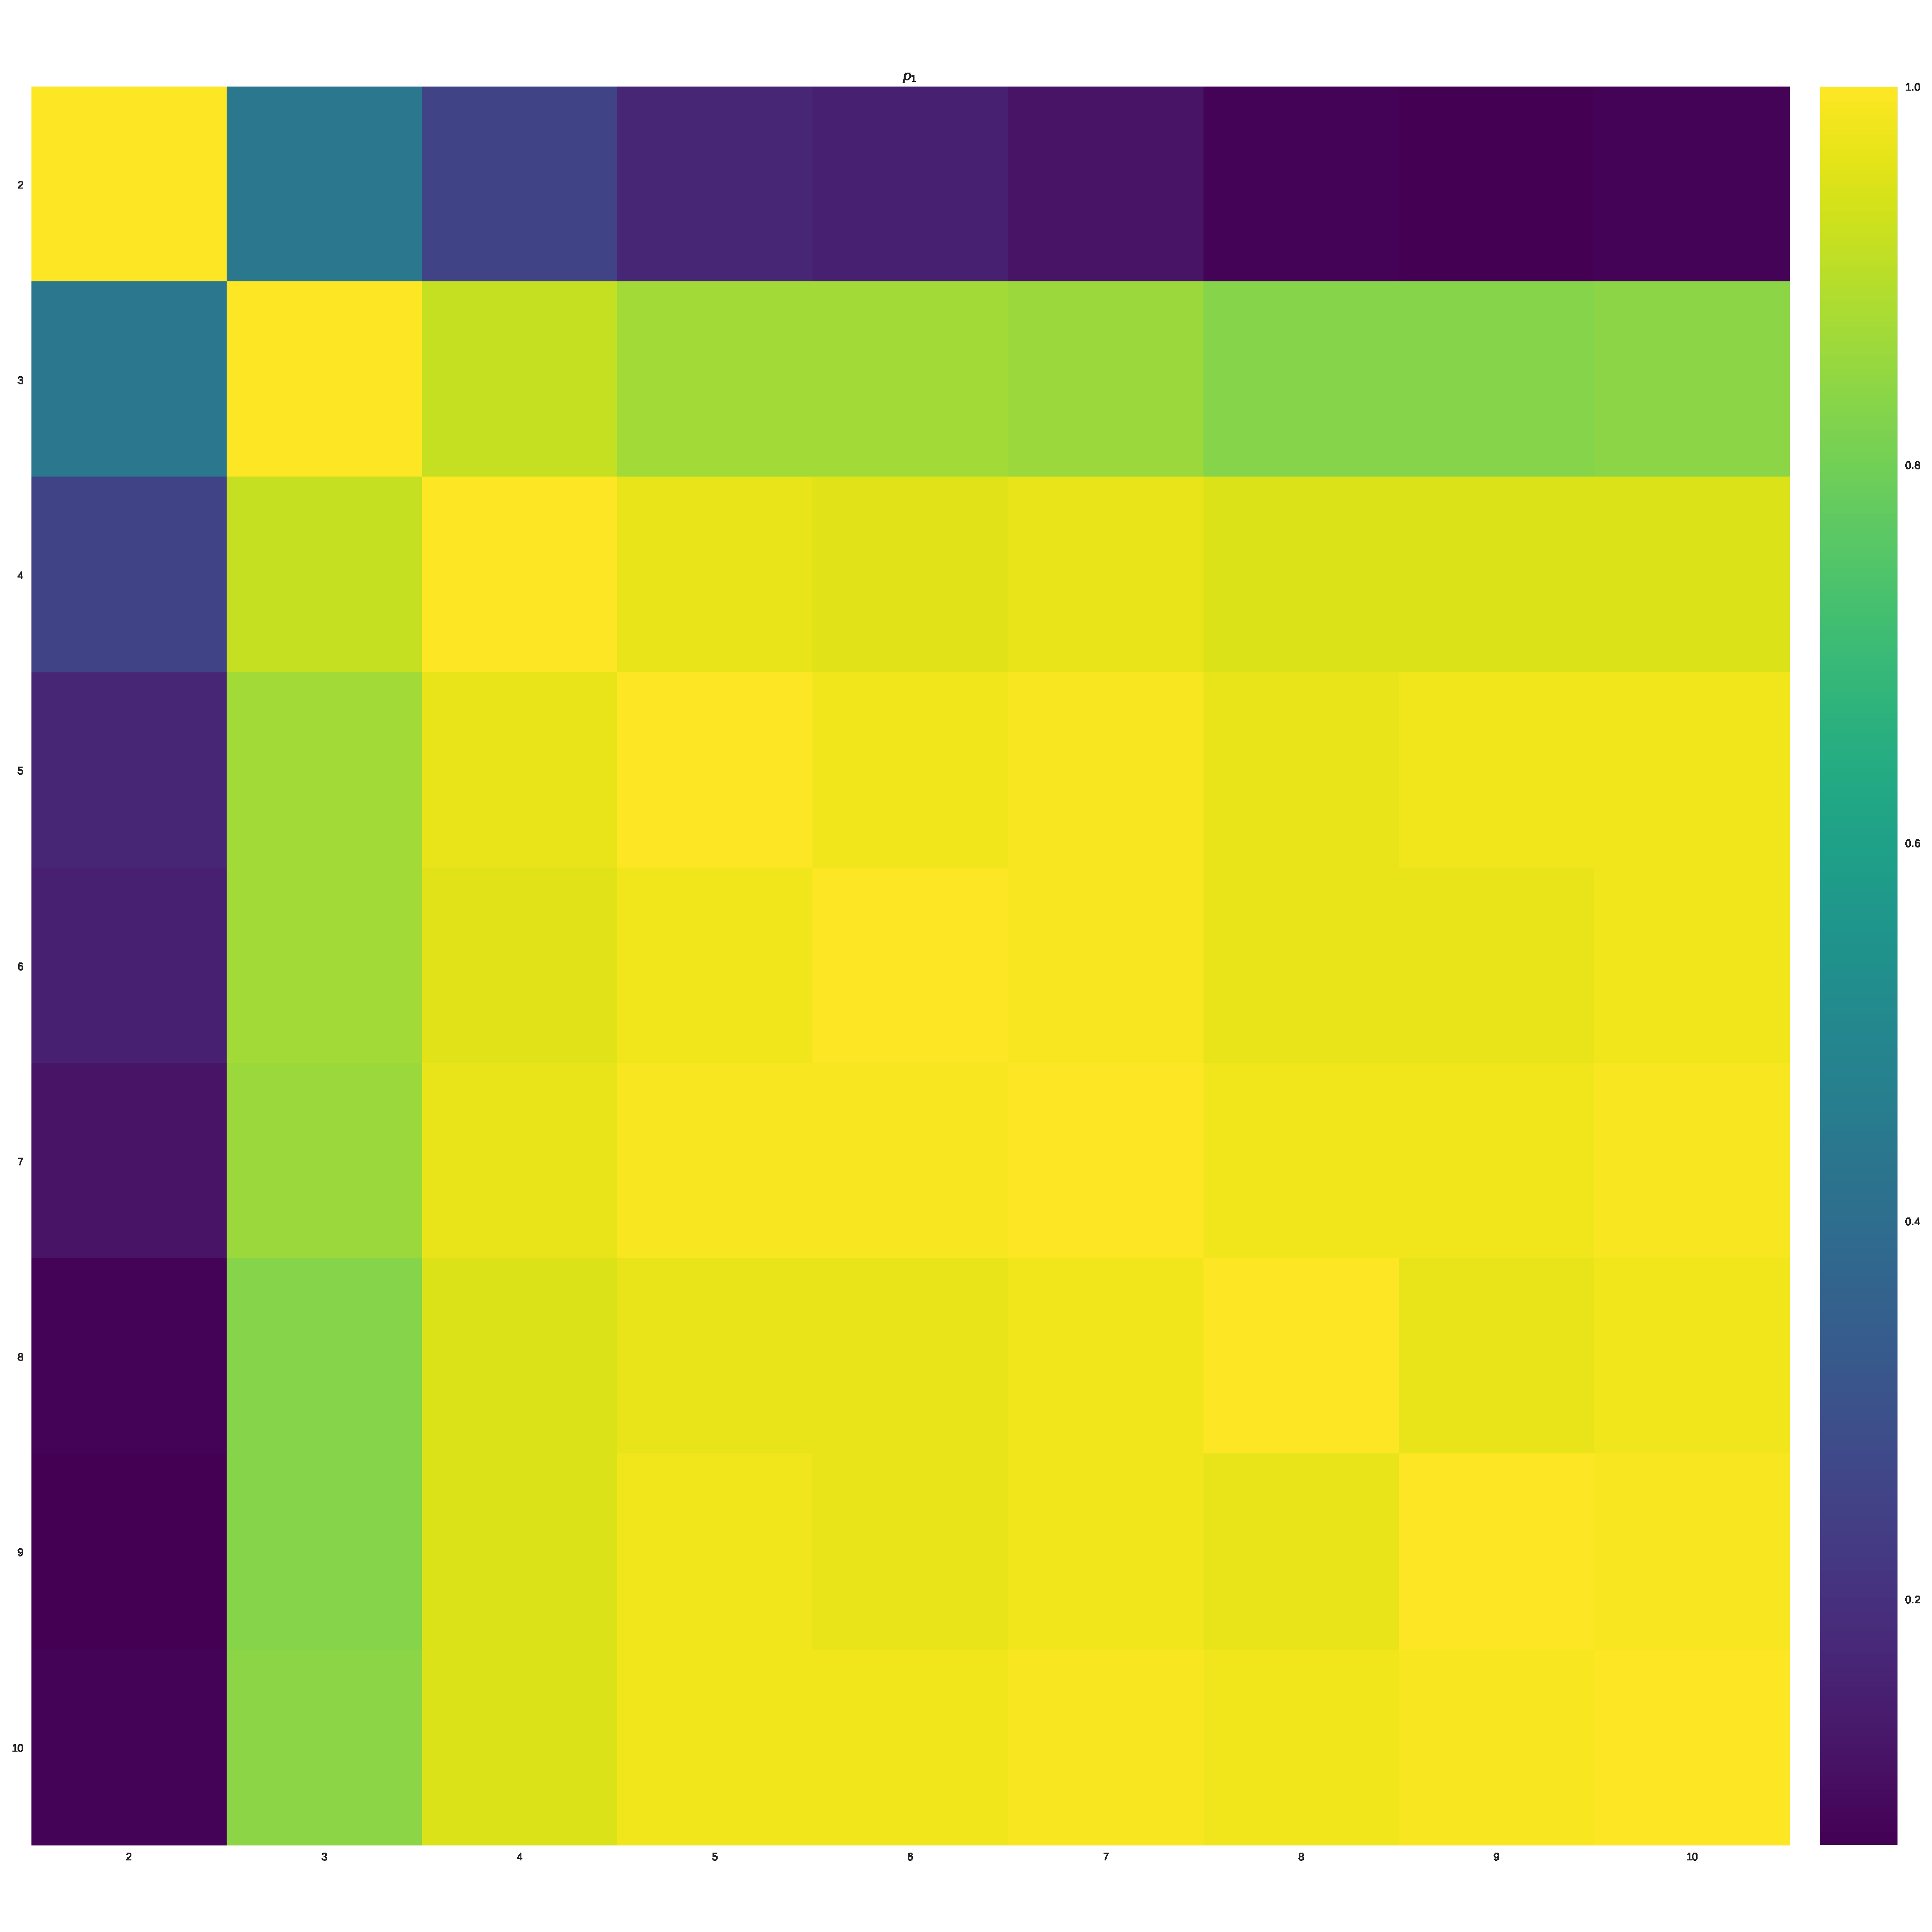
\includegraphics[width=.9\textwidth]{./img/correlation_heatmap_invade.pdf}
		\caption{Rank based on \(x_1\)}
    \end{subfigure}
    ~
	\begin{subfigure}[t]{.3\textwidth}
		\centering
		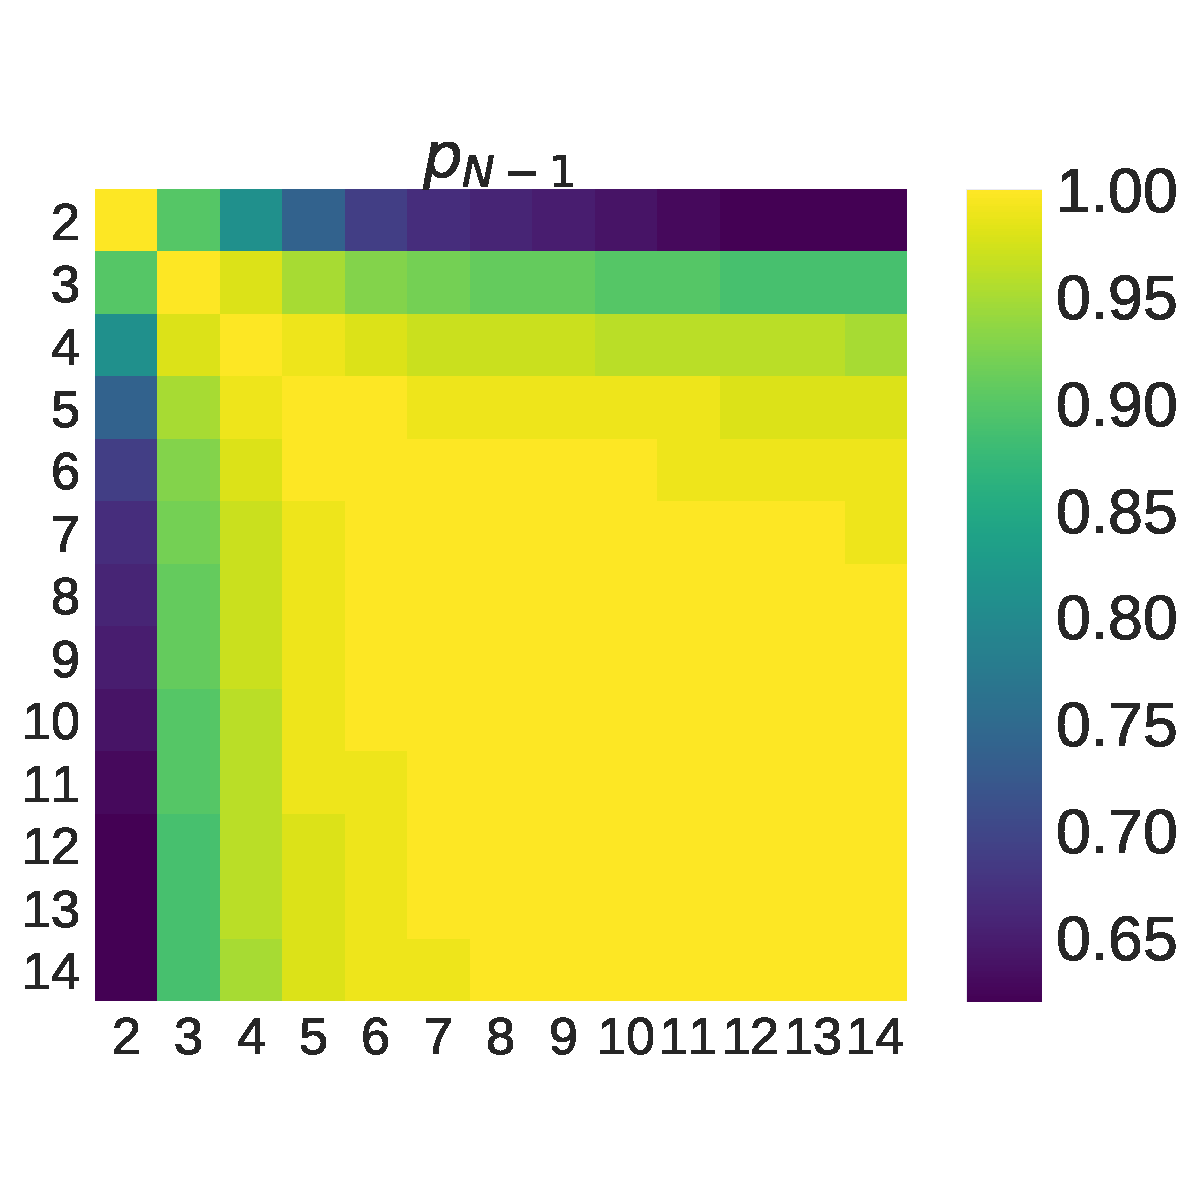
\includegraphics[width=.9\textwidth]{./img/correlation_heatmap_resist.pdf}
        \caption{Rank based on \(x_{N - 1}\)}
    \end{subfigure}
    ~
	\begin{subfigure}[t]{.3\textwidth}
		\centering
		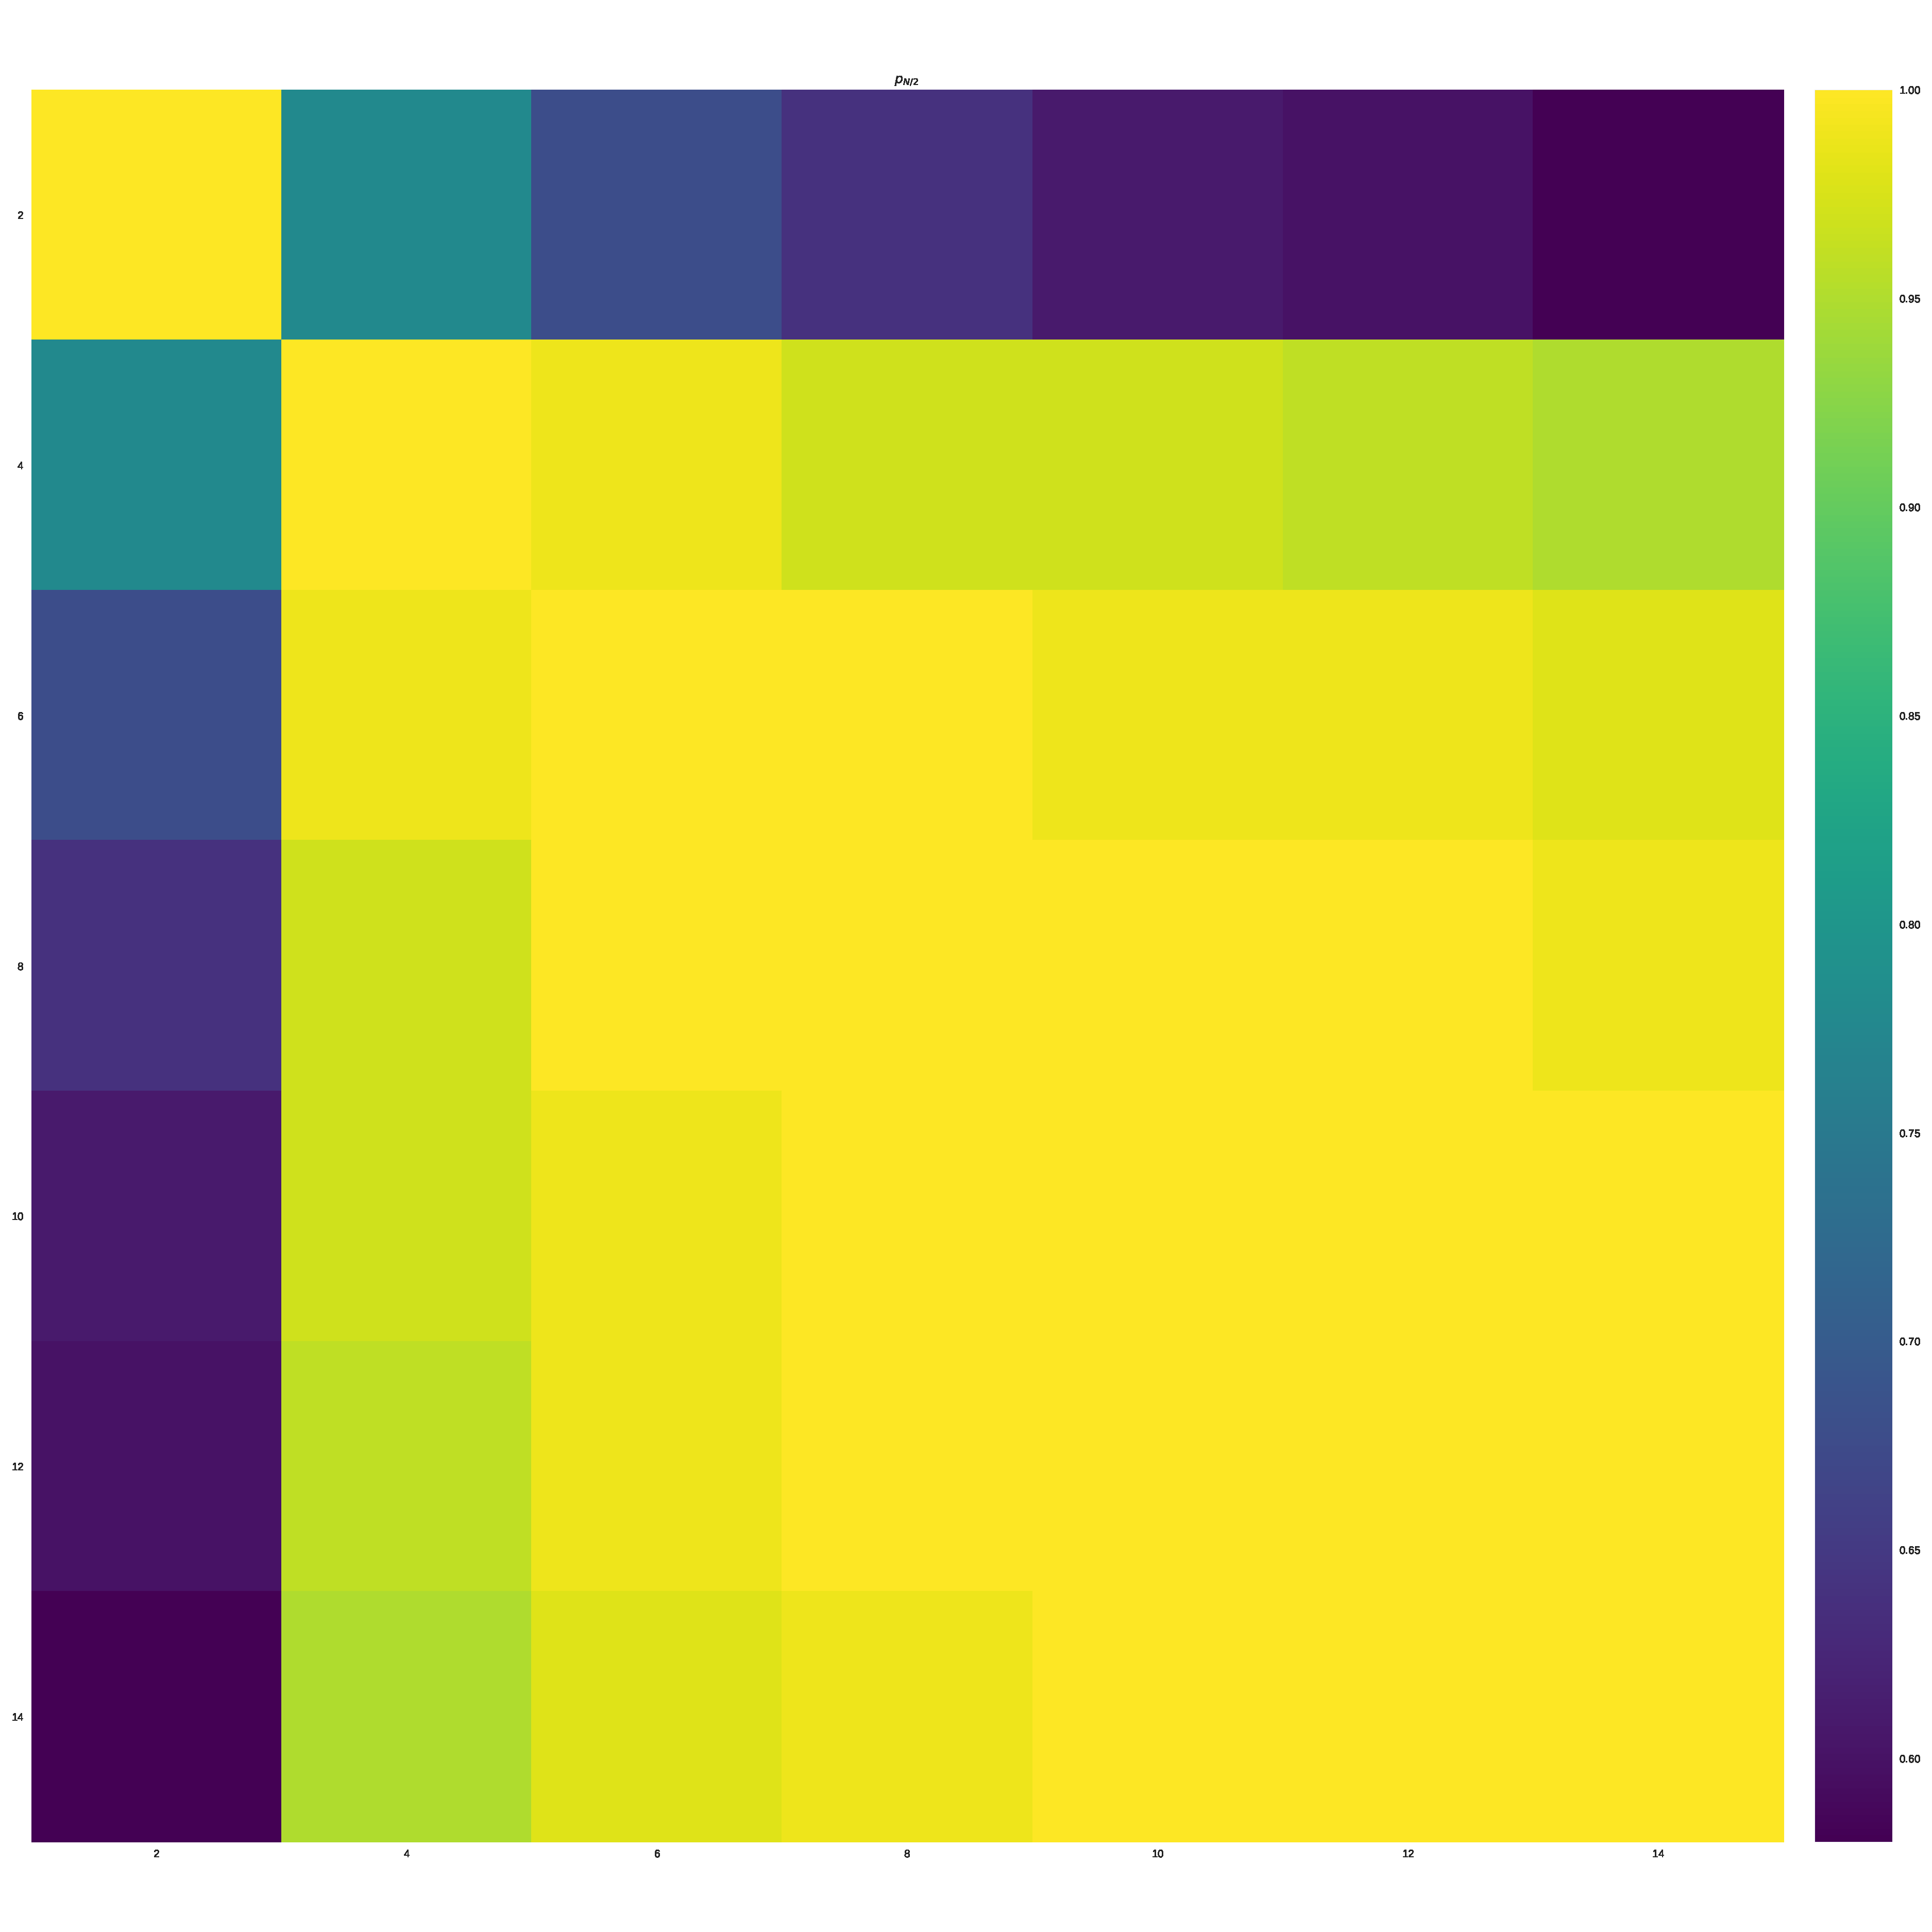
\includegraphics[width=.9\textwidth]{./img/correlation_heatmap_coexist.pdf}
        \caption{Rank based on \(x_{N/2}\)}
    \end{subfigure}
    \caption{Heatmap of correlation coefficients of rankings by population size}
    \label{fig:correlation_coefficients}
\end{figure}

\subsection{Relative fitness}\label{sec:relative_fitness}

% TODO I do not understand the narrative for this and what it adds to the paper.

Under the assumption of a constant relative fitness \(r\) between two
strategies~\cite{Nowak} the formula for \(x_i\) (for given \(N, r\) is:

\begin{equation}\label{equ:fixation_probability_with_constant_relative_fitness}
    x_i = x_i(r) = \frac{1-\frac{1}{r^{i}}}{1-\frac{1}{r^{N}}}
\end{equation}

Figure~\ref{fig:fixation_v_fitness_illustration} shows this function for
\(N=10\) and \(i\in\{1, 5, 10\}\).

\begin{figure}[!hbtp]
    \centering
    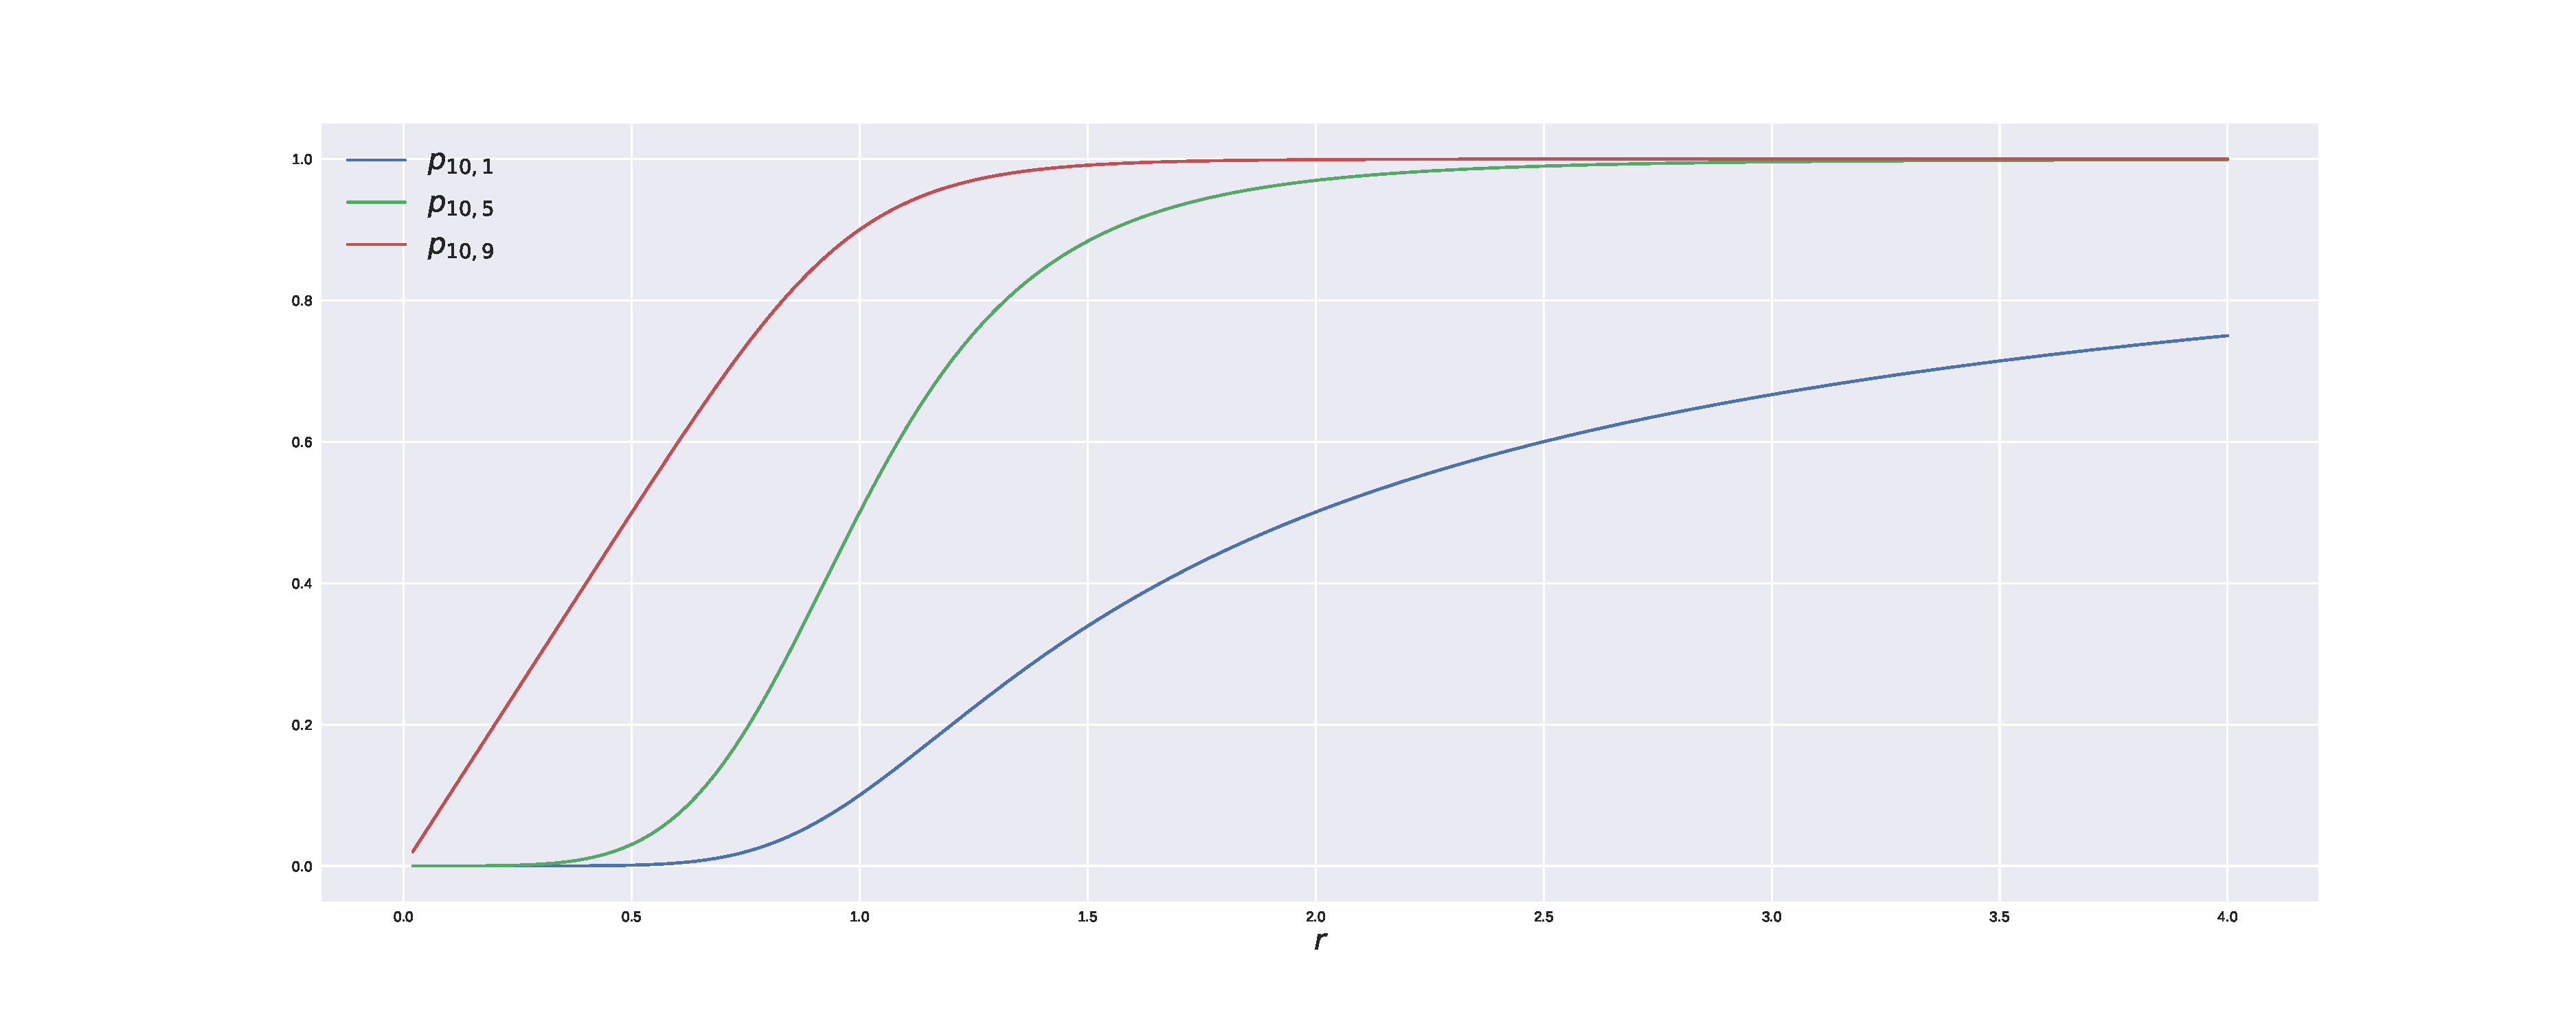
\includegraphics[width=.6\textwidth]{./img/fixation_v_fitness_illustration.pdf}
    \caption{\(x_i(r)\)}
    \label{fig:fixation_v_fitness_illustration}
\end{figure}

The first and second derivative of
(\ref{equ:fixation_probability_with_constant_relative_fitness}) is given by equations
(\ref{equ:fixation_probability_with_constant_relative_fitness_prime}) and
(\ref{equ:fixation_probability_with_constant_relative_fitness_prime2}).

\begin{equation}\label{equ:fixation_probability_with_constant_relative_fitness_prime}
    \frac{dx_i}{dr} = \frac{r^{N - i - 1}}{r^{2 N} - 2 r^{N} + 1} \left(- N r^{i} + N + i r^{N} - i\right)
\end{equation}

\begin{equation}\label{equ:fixation_probability_with_constant_relative_fitness_prime2}
    \frac{d^2x_i}{dr^2} = \frac{r^{N - i - 2}}{\left(r^{N} - 1\right)^{3}} \left(2 N^{2} \left(r^{i} - 1\right) + N \left(r^{N} - 1\right) \left(N \left(r^{i} - 1\right) - 2 i + r^{i} - 1\right) - i \left(i + 1\right) \left(r^{N} - 1\right)^{2}\right)
\end{equation}

Using these, Halley's method \cite{Alefeld2012} can be used to efficiently
numerically invert \(x_i(r)\) to obtain a theoretic relative fitness \(r\) that
gives the calculated \(x_i(r)\) between two strategies for a given \(N, i\).
% TODO Say more things: I still think this is a bit cylic. The formula we are
% using assumes a constant relative fitness which we know does not exist.

\begin{figure}[!hbtp]
    \centering
    \begin{subfigure}[t]{.3\textwidth}
        \centering
        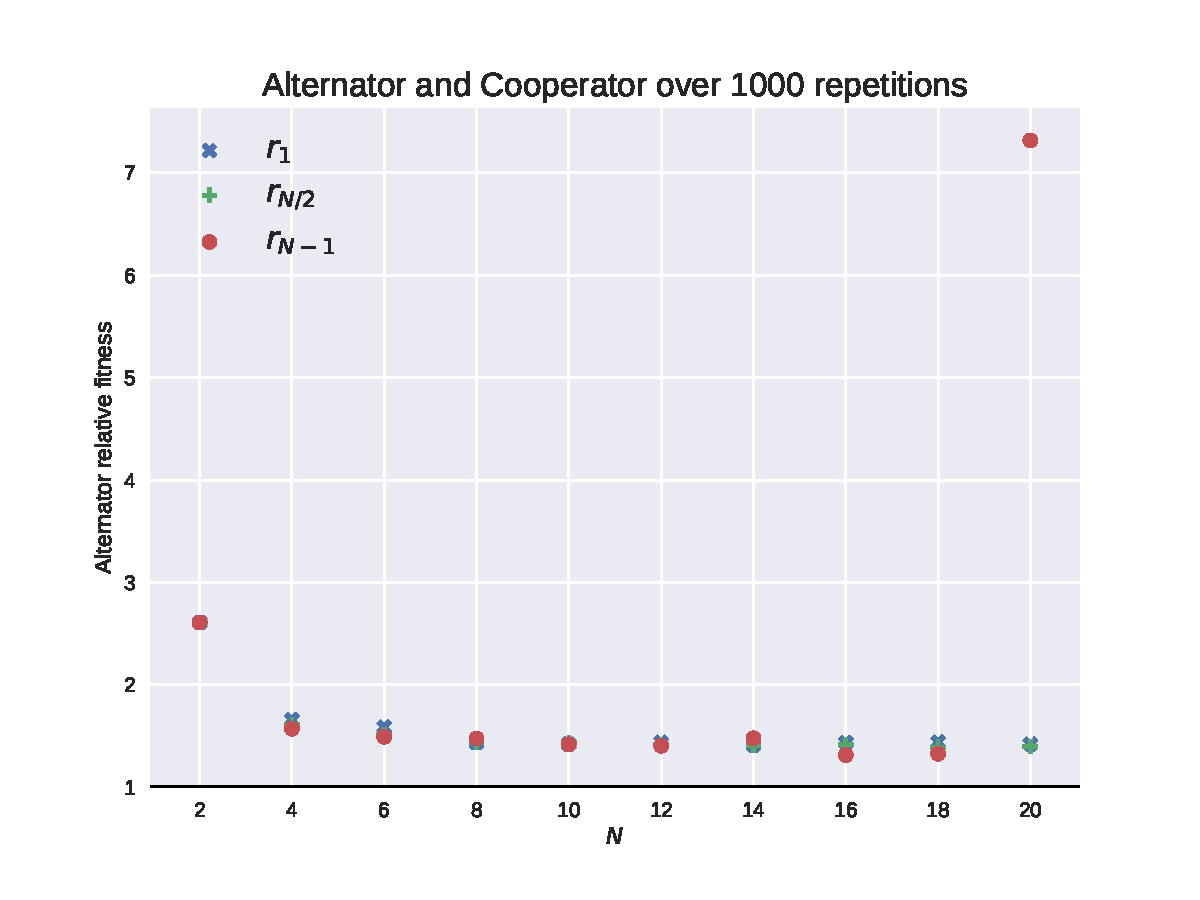
\includegraphics[width=.8\textwidth]{./img/Alternator_v_Cooperator_fitness.pdf}
        \caption{Alternator and Cooperator}
    \end{subfigure}%
    ~
    \begin{subfigure}[t]{.3\textwidth}
        \centering
        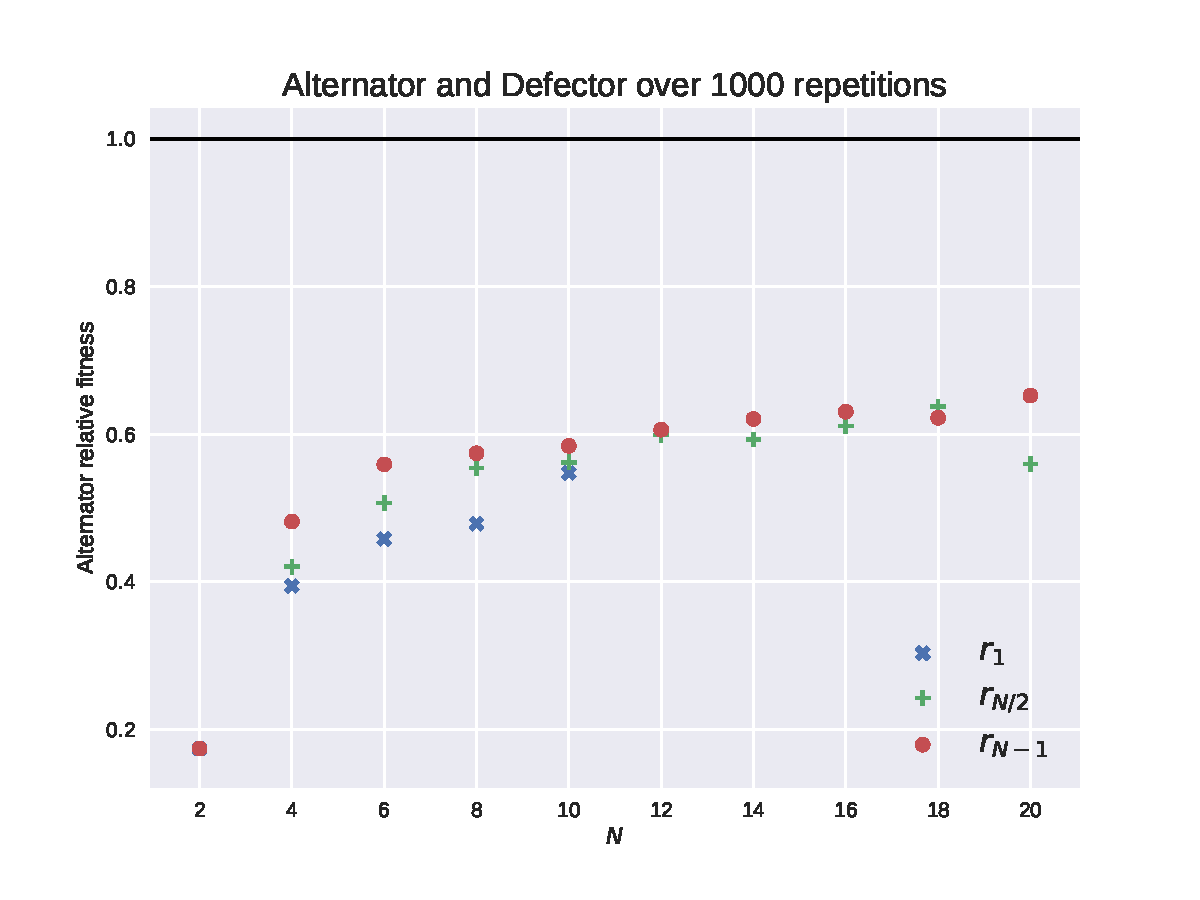
\includegraphics[width=.8\textwidth]{./img/Alternator_v_Defector_fitness.pdf}
        \caption{Alternator and Defector}
    \end{subfigure}%
    ~
    \begin{subfigure}[t]{.3\textwidth}
        \centering
        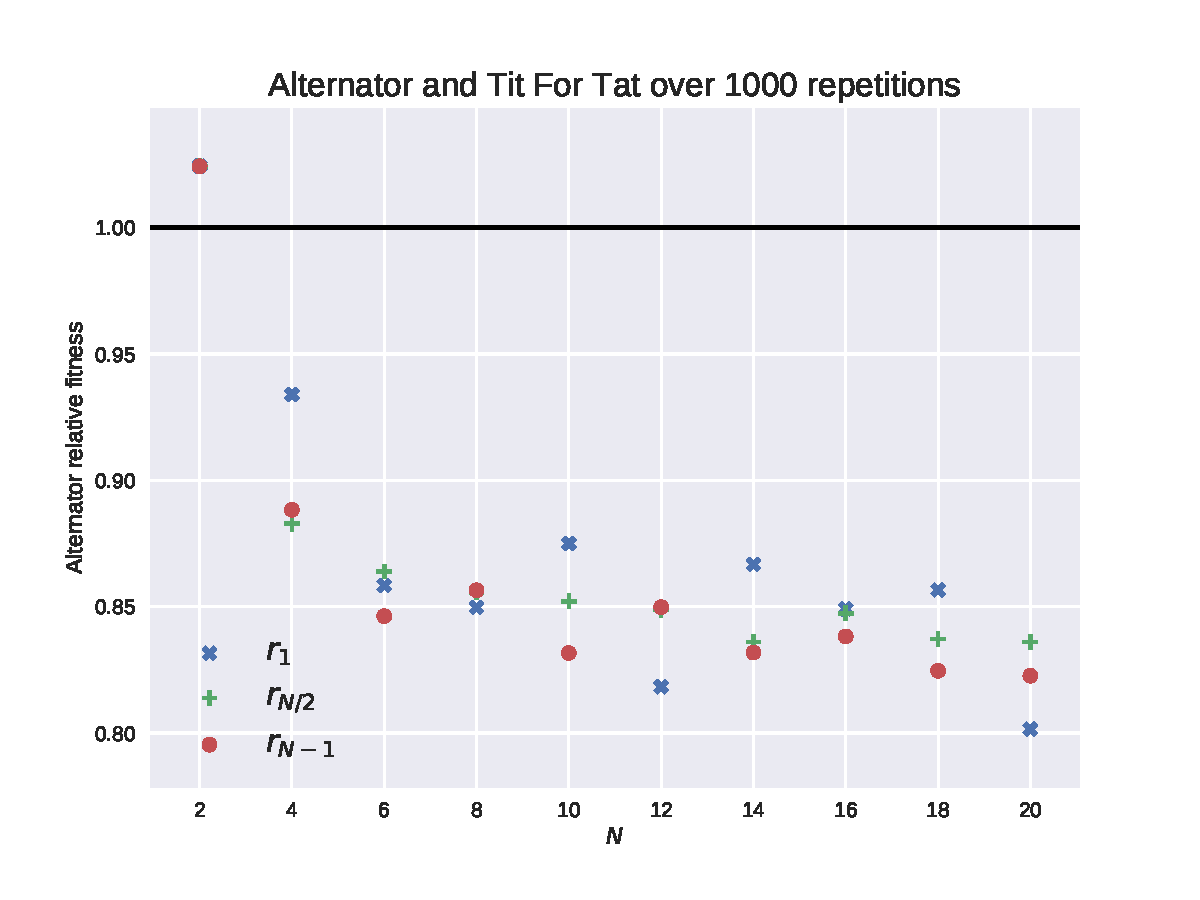
\includegraphics[width=.8\textwidth]{./img/Alternator_v_Tit_For_Tat_fitness.pdf}
        \caption{Alternator and Tit For Tat}
    \end{subfigure}%

    \begin{subfigure}[t]{.3\textwidth}
        \centering
        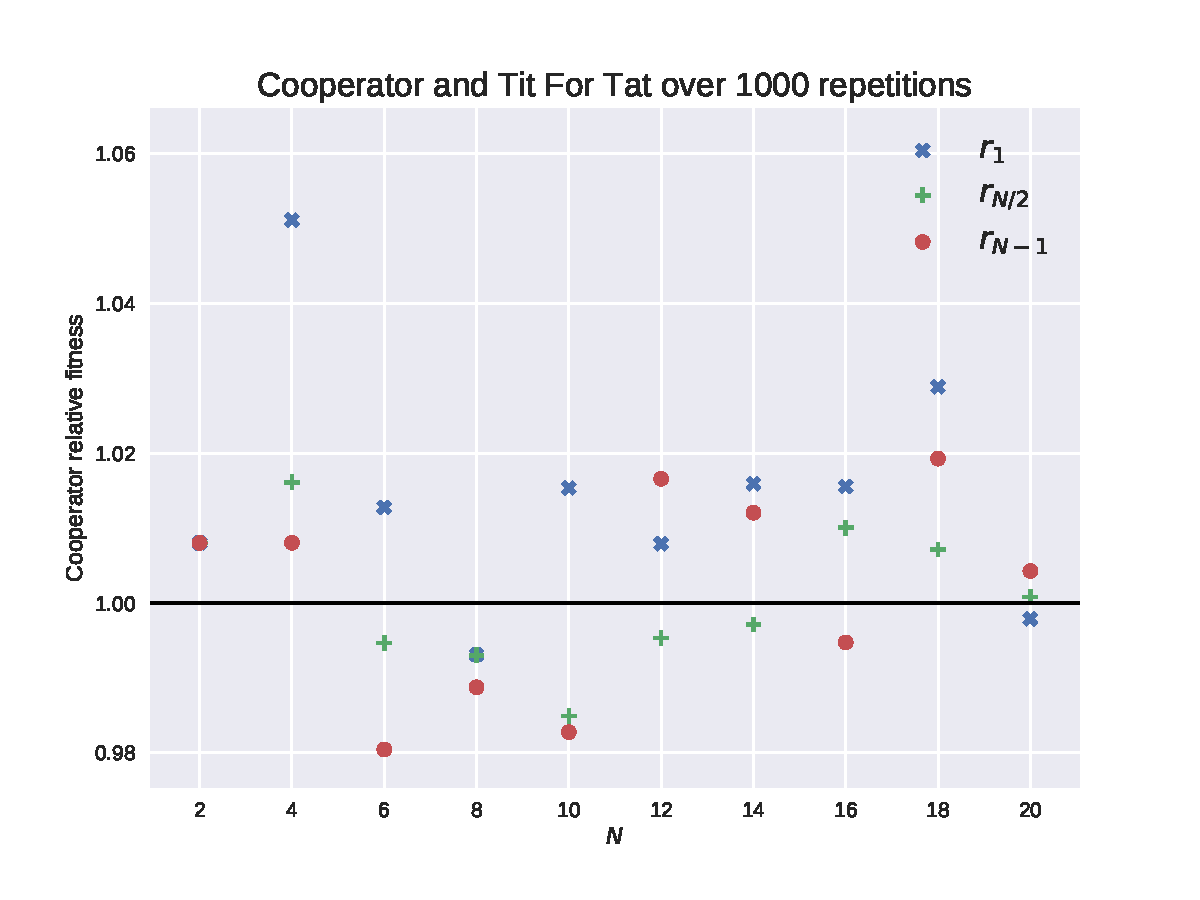
\includegraphics[width=.8\textwidth]{./img/Cooperator_v_Tit_For_Tat_fitness.pdf}
        \caption{Cooperator and Tit For Tat}
    \end{subfigure}%
    ~
    \begin{subfigure}[t]{.3\textwidth}
        \centering
        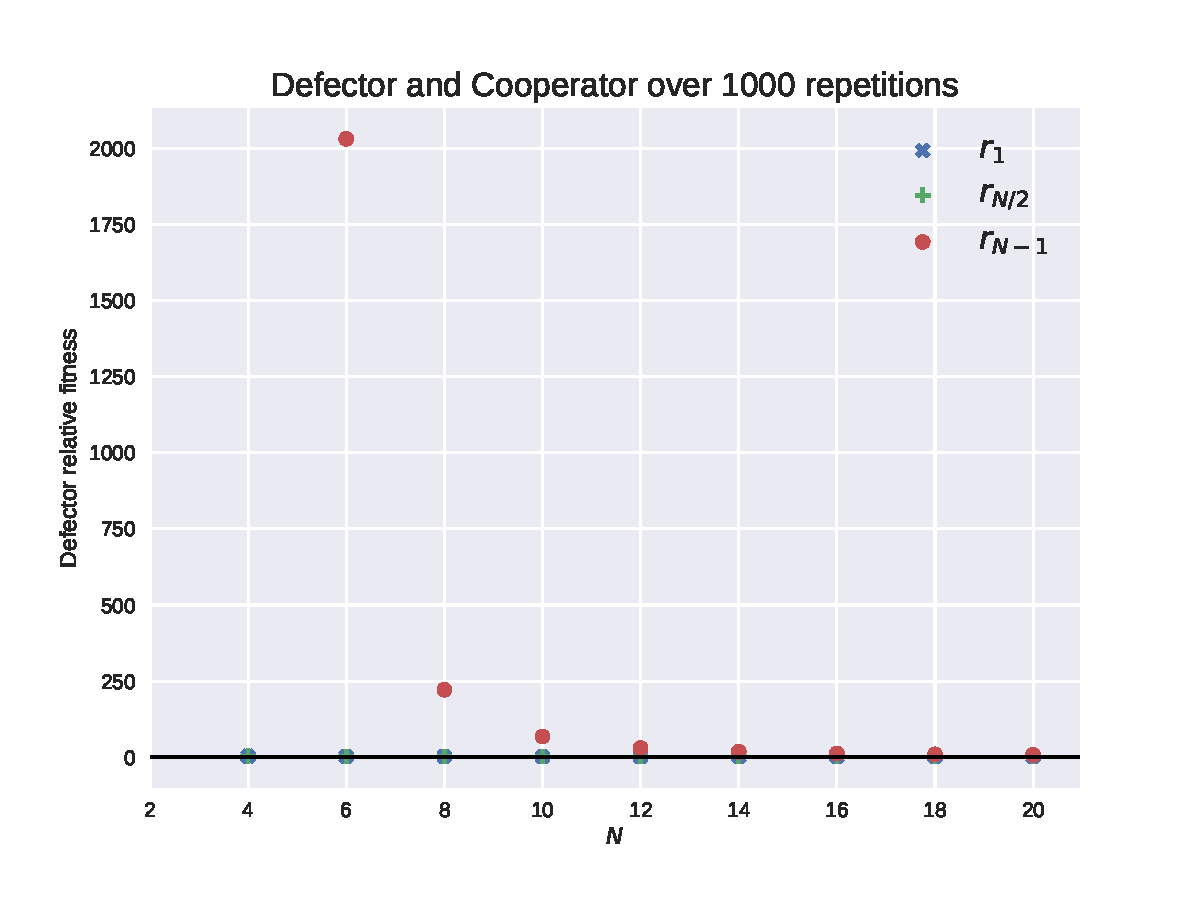
\includegraphics[width=.8\textwidth]{./img/Defector_v_Cooperator_fitness.pdf}
        \caption{Defector and Cooperator}
    \end{subfigure}%
    ~
    \begin{subfigure}[t]{.3\textwidth}
        \centering
        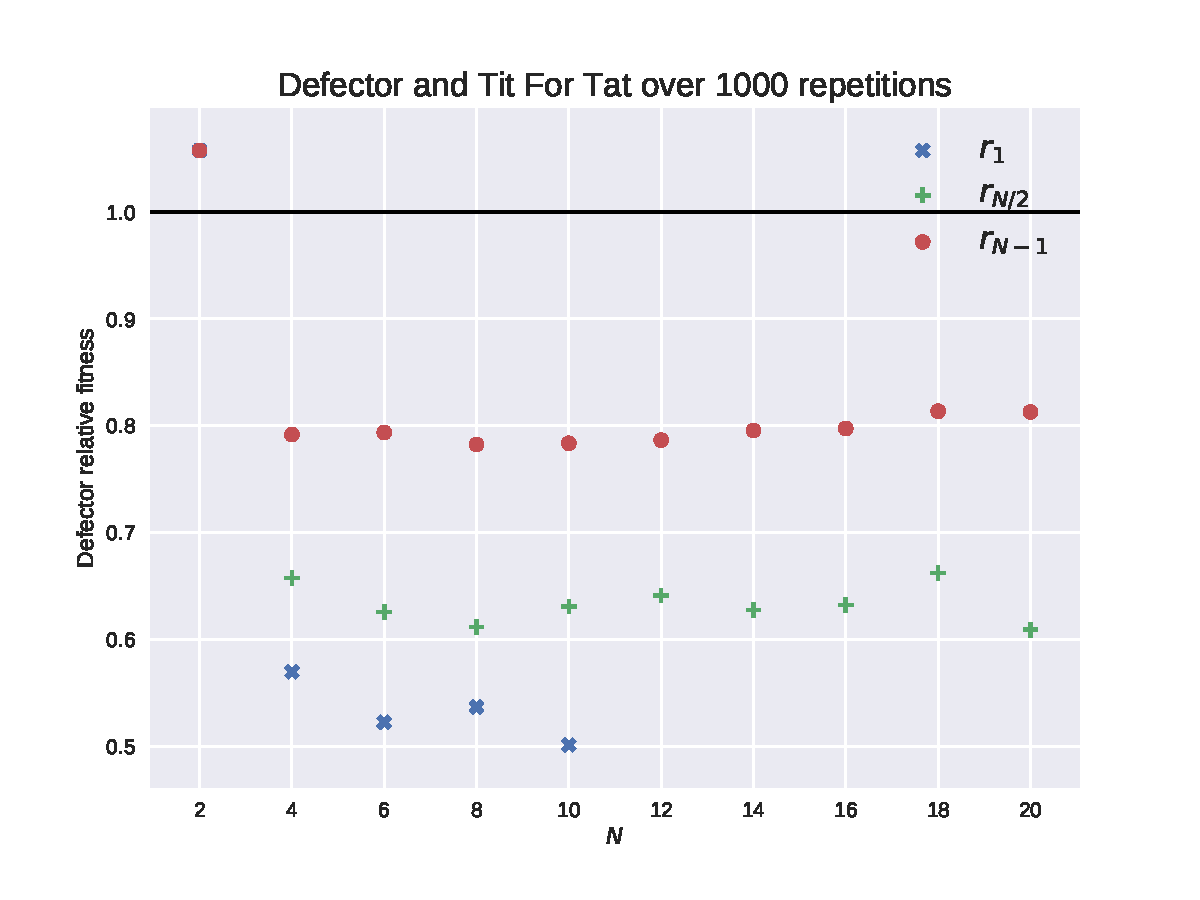
\includegraphics[width=.8\textwidth]{./img/Defector_v_Tit_For_Tat_fitness.pdf}
        \caption{Defector and Tit For Tat}
    \end{subfigure}%

    \begin{subfigure}[t]{.3\textwidth}
        \centering
        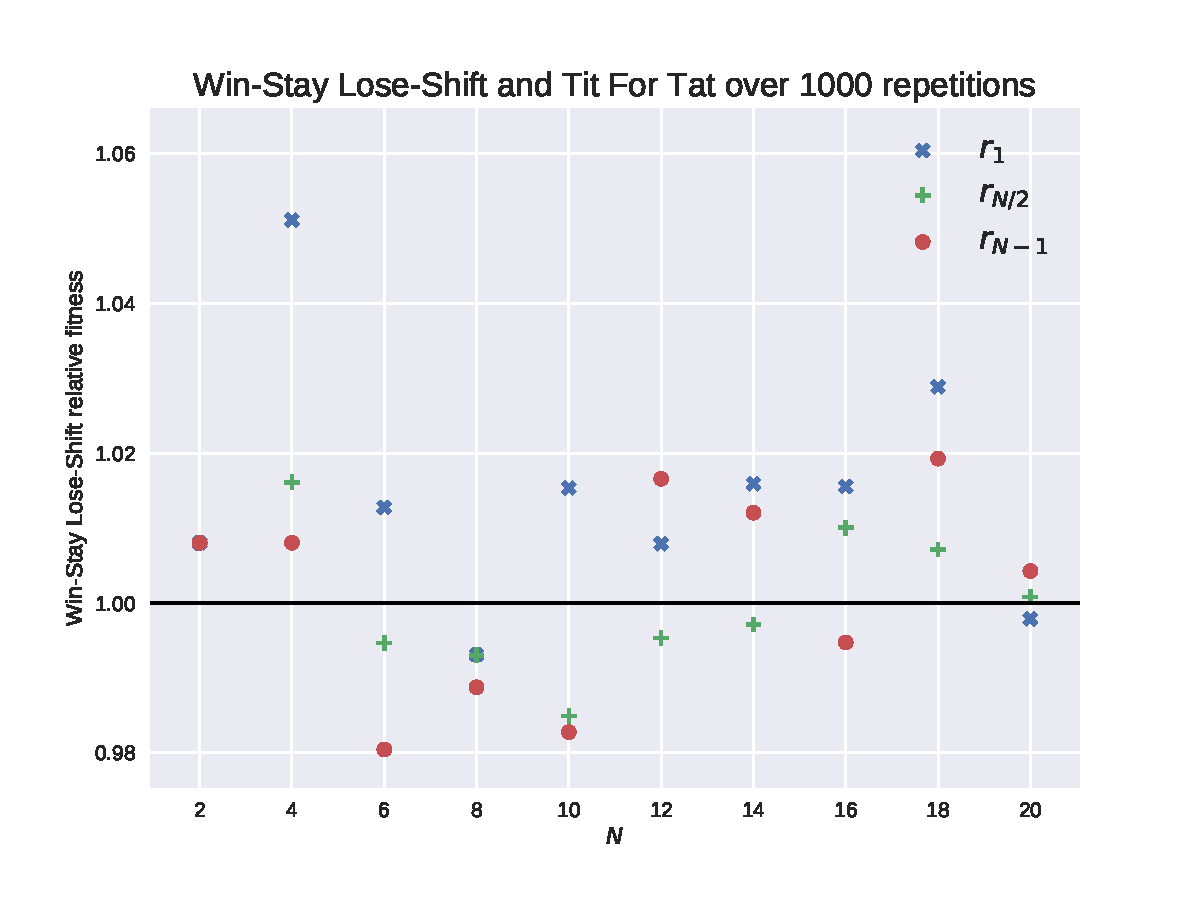
\includegraphics[width=.8\textwidth]{./img/Win-Stay_Lose-Shift_v_Tit_For_Tat_fitness.pdf}
        \caption{Win Stay Lose Shift and Tit For Tat}
    \end{subfigure}%
    ~
    \begin{subfigure}[t]{.3\textwidth}
        \centering
        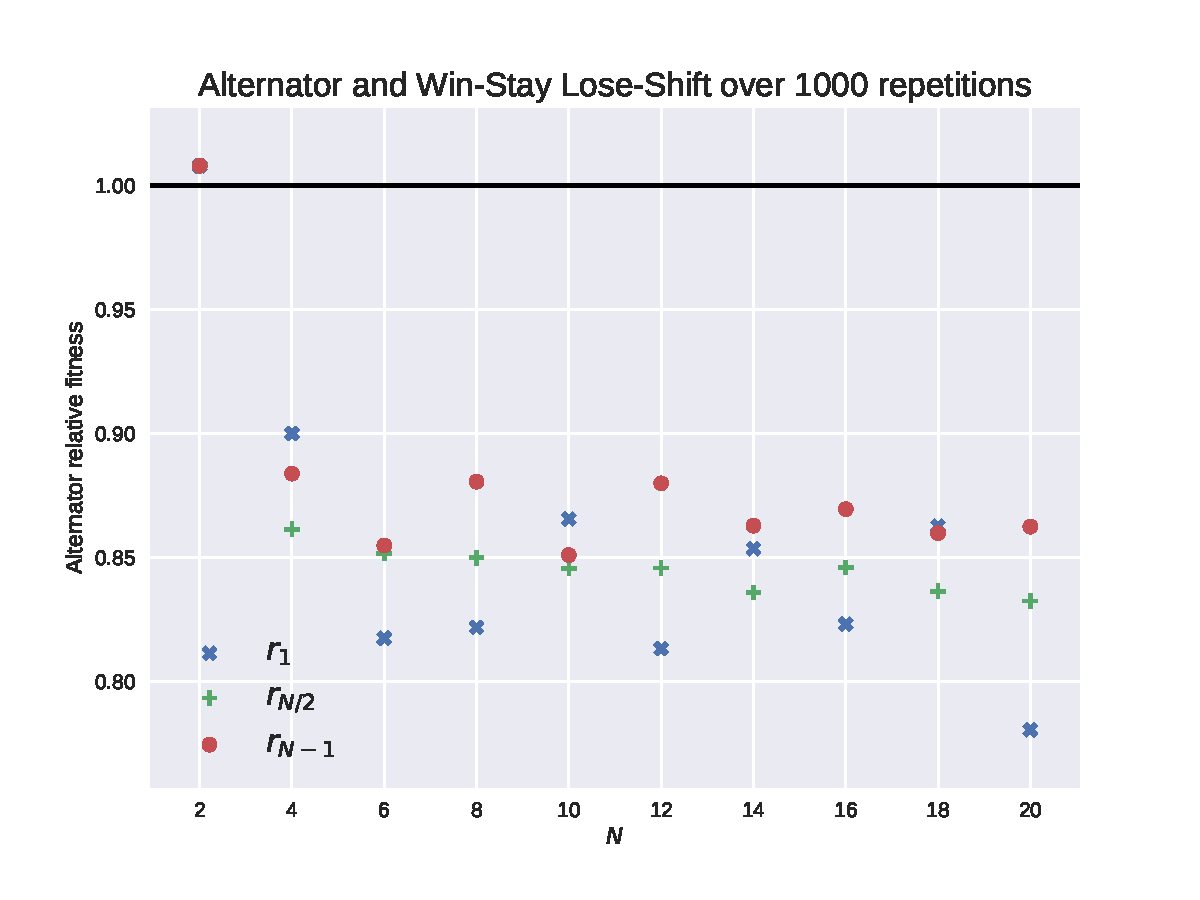
\includegraphics[width=.8\textwidth]{./img/Alternator_v_Win-Stay_Lose-Shift_fitness.pdf}
        \caption{Alternator and Win Stay Lose Shift}
    \end{subfigure}%
    ~
    \begin{subfigure}[t]{.3\textwidth}
        \centering
        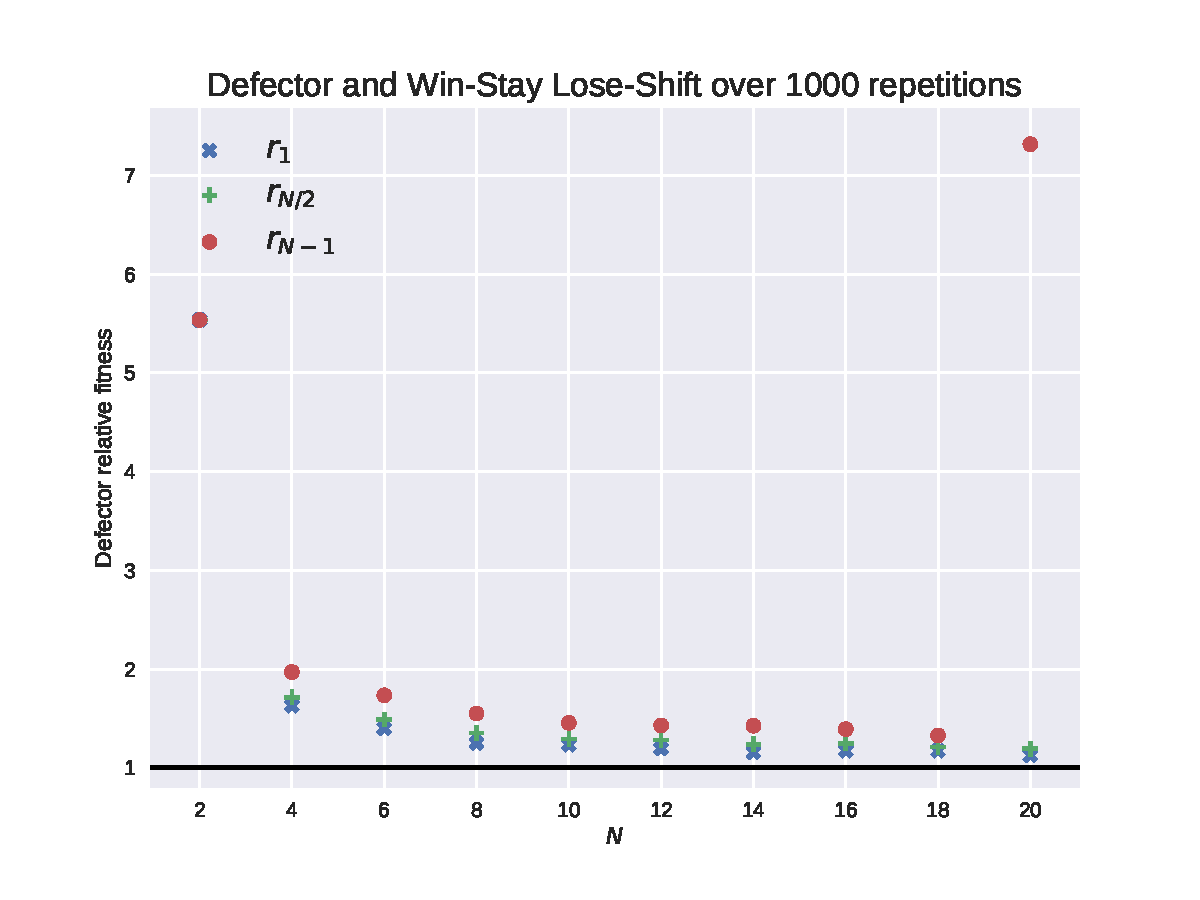
\includegraphics[width=.8\textwidth]{./img/Defector_v_Win-Stay_Lose-Shift_fitness.pdf}
        \caption{Defector and Win Stay Lose Shift}
    \end{subfigure}%
    \caption{Estimated relative fitness
             for \textbf{deterministic} strategies}
    \label{fig:comparison_deterministic}
\end{figure}

\begin{figure}[!hbtp]
    \centering
    \begin{subfigure}[t]{.3\textwidth}
        \centering
        \includegraphics[width=.8\textwidth]{./img/Random_v_Cooperator_fitness.pdf}
        \caption{Random and Cooperator}
    \end{subfigure}%
    ~
    \begin{subfigure}[t]{.3\textwidth}
        \centering
        \includegraphics[width=.8\textwidth]{./img/Random_v_Defector_fitness.pdf}
        \caption{Random and Defector}
    \end{subfigure}%
    ~
    \begin{subfigure}[t]{.3\textwidth}
        \centering
        \includegraphics[width=.8\textwidth]{./img/Random_v_Tit_For_Tat_fitness.pdf}
        \caption{Random and Tit For Tat}
    \end{subfigure}%

    \begin{subfigure}[t]{.3\textwidth}
        \centering
        \includegraphics[width=.8\textwidth]{./img/ALLCorALLD_v_Cooperator_fitness.pdf}
        \caption{All C or all D and Cooperator}
    \end{subfigure}%
    ~
    \begin{subfigure}[t]{.3\textwidth}
        \centering
        \includegraphics[width=.8\textwidth]{./img/ALLCorALLD_v_Defector_fitness.pdf}
        \caption{All C or all D and Defector}
    \end{subfigure}%
    ~
    \begin{subfigure}[t]{.3\textwidth}
        \centering
        \includegraphics[width=.8\textwidth]{./img/Calculator_v_Random_fitness.pdf}
        \caption{Calculator and Random}
    \end{subfigure}%

    \begin{subfigure}[t]{.3\textwidth}
        \centering
        \includegraphics[width=.8\textwidth]{./img/Calculator_v_ALLCorALLD_fitness.pdf}
        \caption{Calculator and All C or all D}
    \end{subfigure}%
    ~
    \begin{subfigure}[t]{.3\textwidth}
        \centering
        \includegraphics[width=.8\textwidth]{./img/Calculator_v_Arrogant_QLearner_fitness.pdf}
        \caption{Calculator and Arrogant Q learner}
    \end{subfigure}%
    ~
    \begin{subfigure}[t]{.3\textwidth}
        \centering
        \includegraphics[width=.8\textwidth]{./img/ALLCorALLD_v_Tit_For_Tat_fitness.pdf}
        \caption{All C or all D and Tit For Tat}
    \end{subfigure}%
    \caption{Estimated relative fitness
             for \textbf{stochastic} strategies}
    \label{fig:comparison_stochastic}
\end{figure}


\section{Conclusion}\label{sec:conclusion}

A detailed empirical analysis of 164 strategies of the IPD within a pairwise
Moran process has been carried out. All \(\binom{164}{2}=13,366\) possible
ordered pairs of strategies have been placed in a Moran process with different
starting values allowing the each strategy to attempt to invade the other.

This is the largest such experiment carried out and has lead to many insights.

When studying evolutionary processes it is vital to consider \(N>2\) as the
special case for \(N=2\) cannot be used to extrapolate performance in bigger
populations. This was shown both observationally in
Sections~\ref{sec:strong_invaders} and~\ref{sec:strong_resistors} but also by
considering the correlation of the ranks in different population sizes in
Section~\ref{sec:population_size}.

For \(N=2\), memory one strategies perform well, in particular as predicted by
\cite{Press2012} zero determinant strategies rank highly. However, there are no
memory one strategies in the top 5 performing strategies for \(N>3\). This is
due to their lack of sophistication which allows them to recognise and adjust to
their opponent.

It is felt that these findings are important for the ongoing understanding of
population dynamics and offer evidence for some of the shortcomings of short
memory which has started to be recognised by the community~\cite{Hilbe2017}.

All source code for this work has been written in a sustainable manner: it is
open source, under version control and tested which ensures that all results can
be reproduced \cite{Prlic2012, Sandve2013, Wilson2014}. The raw data as well as
the processed data has also been properly archived.

There are various areas for further work to build on this. Firstly, an analysis
of the effect of noise would offer insights about the stability of the findings.
It would also be possible to consider three or more types of strategy in the
population and finally mutation would also offer an interesting dimension to
explore.

\section*{Acknowledgements}

This work was performed using the computational facilities of the Advanced
Research Computing @ Cardiff (ARCCA) Division, Cardiff University.

A variety of software libraries have been used in this work:

\begin{itemize}
    \item The Axelrod library (IPD strategies and Moran processes)
        \cite{axelrodproject}.
    \item The matplotlib library (visualisation) \cite{hunter2007matplotlib}.
    \item The pandas and numpy libraries (data manipulation)
        \cite{mckinney2010data, walt2011numpy}.
\end{itemize}

\printbibliography

\appendix

\section{List of players}\label{app:list_of_players}

\begin{multicols}{3}
	\begin{enumerate}
		\item $\phi$
\item $\pi$
\item $e$
\item ALLCorALLD
\item Adaptive
\item Adaptive Pavlov 2006
\item Adaptive Pavlov 2011
\item Adaptive Tit For Tat: 0.5
\item Aggravater
\item Alternator
\item Alternator Hunter
\item Anti Tit For Tat
\item AntiCycler
\item Appeaser
\item Arrogant QLearner
\item Average Copier
\item Better and Better
\item Bully
\item Calculator
\item Cautious QLearner
\item CollectiveStrategy
(\textbf{CS})\item Contrite Tit For Tat
\item Cooperator
\item Cooperator Hunter
\item Cycle Hunter
\item Cycler CCCCCD
\item Cycler CCCD
\item Cycler CCCDCD
\item Cycler CCD
\item Cycler DC
\item Cycler DDC
\item Davis: 10
\item Defector
\item Defector Hunter
\item Desperate
\item Doubler
\item EasyGo
\item Eatherley
\item Eventual Cycle Hunter
\item Evolved ANN
\item Evolved ANN 5
\item Evolved ANN 5 Noise 05
\item Evolved FSM 16
\item Evolved FSM 16 Noise 05
\item Evolved FSM 4
\item Evolved HMM 5
\item EvolvedLookerUp1\_1\_1
\item EvolvedLookerUp2\_2\_2
\item FSM Player: [(0, 'C', 0, 'C'), (0, 'D', 3, 'C'), (1, 'C', 5, 'D'), (1, 'D', 0, 'C'), (2, 'C', 3, 'C'), (2, 'D', 2, 'D'), (3, 'C', 4, 'D'), (3, 'D', 6, 'D'), (4, 'C', 3, 'C'), (4, 'D', 1, 'D'), (5, 'C', 6, 'C'), (5, 'D', 3, 'D'), (6, 'C', 6, 'D'), (6, 'D', 6, 'D'), (7, 'C', 7, 'D'), (7, 'D', 5, 'C')], 1, C
(\textbf{Trained FSM 1})\item FSM Player: [(0, 'C', 13, 'D'), (0, 'D', 12, 'D'), (1, 'C', 3, 'D'), (1, 'D', 4, 'D'), (2, 'C', 14, 'D'), (2, 'D', 9, 'D'), (3, 'C', 0, 'C'), (3, 'D', 1, 'D'), (4, 'C', 1, 'D'), (4, 'D', 2, 'D'), (5, 'C', 12, 'C'), (5, 'D', 6, 'C'), (6, 'C', 1, 'C'), (6, 'D', 14, 'D'), (7, 'C', 12, 'D'), (7, 'D', 2, 'D'), (8, 'C', 7, 'D'), (8, 'D', 9, 'D'), (9, 'C', 8, 'D'), (9, 'D', 0, 'D'), (10, 'C', 2, 'C'), (10, 'D', 15, 'C'), (11, 'C', 7, 'D'), (11, 'D', 13, 'D'), (12, 'C', 3, 'C'), (12, 'D', 8, 'D'), (13, 'C', 7, 'C'), (13, 'D', 10, 'D'), (14, 'C', 10, 'D'), (14, 'D', 7, 'D'), (15, 'C', 15, 'C'), (15, 'D', 11, 'D')], 1, C
(\textbf{Trained FSM 2})\item FSM Player: [(0, 'C', 7, 'C'), (0, 'D', 1, 'C'), (1, 'C', 11, 'D'), (1, 'D', 11, 'D'), (2, 'C', 8, 'D'), (2, 'D', 8, 'C'), (3, 'C', 3, 'C'), (3, 'D', 12, 'D'), (4, 'C', 6, 'C'), (4, 'D', 3, 'C'), (5, 'C', 11, 'C'), (5, 'D', 8, 'D'), (6, 'C', 13, 'D'), (6, 'D', 14, 'C'), (7, 'C', 4, 'D'), (7, 'D', 2, 'D'), (8, 'C', 14, 'D'), (8, 'D', 8, 'D'), (9, 'C', 0, 'C'), (9, 'D', 10, 'D'), (10, 'C', 8, 'C'), (10, 'D', 15, 'C'), (11, 'C', 6, 'D'), (11, 'D', 5, 'D'), (12, 'C', 6, 'D'), (12, 'D', 9, 'D'), (13, 'C', 9, 'D'), (13, 'D', 8, 'D'), (14, 'C', 8, 'D'), (14, 'D', 13, 'D'), (15, 'C', 4, 'C'), (15, 'D', 5, 'C')], 1, C
(\textbf{Trained FSM 3})\item Feld: 1.0, 0.5, 200
\item Firm But Fair
\item Fool Me Forever
\item Fool Me Once
\item Forgetful Fool Me Once: 0.05
\item Forgetful Grudger
\item Forgiver
\item Forgiving Tit For Tat
\item Fortress3
\item Fortress4
\item GTFT: 0.33
\item General Soft Grudger: n=1,d=4,c=2
\item Gradual
\item Gradual Killer: ('D', 'D', 'D', 'D', 'D', 'C', 'C')
\item Grofman
\item Grudger
\item GrudgerAlternator
\item Grumpy: Nice, 10, -10
\item Handshake
\item Hard Go By Majority
\item Hard Go By Majority: 10
\item Hard Go By Majority: 20
\item Hard Go By Majority: 40
\item Hard Go By Majority: 5
\item Hard Prober
\item Hard Tit For 2 Tats
\item Hard Tit For Tat
\item Hesitant QLearner
\item Hopeless
\item Inverse
\item Inverse Punisher
\item Joss: 0.9
\item Level Punisher
\item Limited Retaliate 2: 0.08, 15
\item Limited Retaliate 3: 0.05, 20
\item Limited Retaliate: 0.1, 20
\item MEM2
\item Math Constant Hunter
\item Meta Hunter Aggressive: 7 players
\item Meta Hunter: 6 players
\item Naive Prober: 0.1
\item Negation
\item Nice Average Copier
\item Nydegger
\item Omega TFT: 3, 8
\item Once Bitten
\item Opposite Grudger
\item PSO Gambler 1\_1\_1
\item PSO Gambler 2\_2\_2
\item PSO Gambler 2\_2\_2 Noise 05
\item PSO Gambler Mem1
\item Predator
\item Prober
\item Prober 2
\item Prober 3
\item Prober 4
\item Pun1
\item Punisher
\item Raider
\item Random Hunter
\item Random: 0.5
\item Remorseful Prober: 0.1
\item Resurrection
\item Retaliate 2: 0.08
\item Retaliate 3: 0.05
\item Retaliate: 0.1
\item Revised Downing: True
\item Ripoff
\item Risky QLearner
\item SelfSteem
\item ShortMem
\item Shubik
\item Slow Tit For Two Tats
\item Slow Tit For Two Tats 2
\item Sneaky Tit For Tat
\item Soft Go By Majority
\item Soft Go By Majority: 10
\item Soft Go By Majority: 20
\item Soft Go By Majority: 40
\item Soft Go By Majority: 5
\item Soft Grudger
\item Soft Joss: 0.9
\item SolutionB1
\item SolutionB5
\item Spiteful Tit For Tat
\item Stochastic Cooperator
\item Stochastic WSLS: 0.05
\item Suspicious Tit For Tat
\item Tester
\item ThueMorse
\item ThueMorseInverse
\item Thumper
\item Tit For 2 Tats
(\textbf{Tf2T})\item Tit For Tat
(\textbf{TfT})\item Tricky Cooperator
\item Tricky Defector
\item Tullock: 11
\item Two Tits For Tat
(\textbf{2TfT})\item VeryBad
\item Willing
\item Win-Shift Lose-Stay: D
\item Win-Stay Lose-Shift: C
(\textbf{WSLS})\item Winner12
\item Winner21
\item Worse and Worse
\item Worse and Worse 2
\item Worse and Worse 3
\item ZD-Extort-2 v2: 0.125, 0.5, 1
\item ZD-Extort-2: 0.1111111111111111, 0.5
\item ZD-Extort-4: 0.23529411764705882, 0.25, 1
\item ZD-GEN-2: 0.125, 0.5, 3
\item ZD-GTFT-2: 0.25, 0.5
\item ZD-SET-2: 0.25, 0.0, 2

	\end{enumerate}
\end{multicols}

\end{document}
